\chapter{自動運転システムの開発}
\section{はじめに}

自律移動ロボットの開発プロセスにおいて、実環境における実証実験が数多く行われている。
特に、屋外における自律移動においては、シミュレーションと実環境では、制約や環境条件が全く異なるため、実環境のみでしか得ることのできない知見が多く、自律移動の実用化に向けては、実機を用いた実証実験が必要とされている。
実証実験に代表されるつくばチャレンジでは、自律移動ロボットの設計において、要素技術であるLiDARを中心とした、センサ系の使用が主となり、複数のセンサとの融合(センサフュージョン)による環境認識の高精度化が図られている。
それと同時に、自律移動ロボットの実用化に向けて、使用されるセンサの選定、用途に応じて最適化する試みが行われている。
特に、ロボットに搭載するセンサの使用数を少なくすることは、ロボットに課される制約・条件、ソフトウェア開発の工数減、保守性の向上のために、考慮すべき点と述べられている。
自律移動チャレンジの参加車両の形態は多様であり、差動二輪型が一般的であるが、パーソナルビークル等の使用としては、4輪車両型の自律移動等も見られる。
自律移動の要素技術は、自動運転にも使用されているが、つくばチャレンジでは、人と共存するロボットとして比較的低速であることが特徴であり、LiDARセンサによる環境認識の比重が高い。
対して、自動運転では、カメラや深度センサ等のイメージセンサ等のコンピュータビジョンとLiDARセンサによるSLAMがそれぞれ同じ割合での併用が標準となり、センサ融合に関する技術について言及されている。
自律移動ロボットの要素技術として用いられているLiDARのメーカーとして有名な北陽電機株式会社は、中之島チャレンジに参加し、自律移動ロボットの実機を開発して、実際にフィールドで議論を行うことで、新製品の開発を行っている。自律移動ロボットの要素技術であるLiDARの開発においても、実証実験が不可欠である。
筆者は、中之島ロボットチャレンジを観戦することで、将来的に自律移動ロボットやLiDARの開発に携わりたいと考えた。
今回は、縁あって北陽電機株式会社様よりLiDARを貸与頂き、有効活用して筆者自らの開発アイデアを実現することを目標として研究に取り組むこととした。
本研究の位置付けは、LiDARの使用技術の勉強並びに、北陽電機株式会社様への就職を目的としている。

\section{従来研究}
\subsection{つくばチャレンジの屋外ナビゲーションシステム}
つくばチャレンジ\cite{auto:tsukuba}は、自律移動ロボットのナビゲーション技術の発展を目的とした実験走行会である。
この期間は実験走行の機会が定期的に用意され、最終日に本走行(最終実証走行)が行われる。
課題として、つくば市の屋外環境において約1[km]の自律走行コースが設定される。
コースには、遊歩道、公園、広場、車道に面した一般歩道、湾曲路、陸橋、狭いゲート、自動ドアなど多様な環境を含む。
ロボットのために環境に手を加えることは許されず、歩行者や自転車などが存在する実環境のままで行われる。
ただし、安全確保のため、一部の交差点で一時停止を行うことが規定されている。
つくばチャレンジのコースを自律走行するには、目的地と現在地を認識する自己位置推定、歩行者や他のロボットとの衝突を防ぐ障害物検出・回避が高い確実性で求められる。

友納ら\cite{auto:tomonoh}は、屋外での自律走行が現状でどのくらい可能かを実環境で見極めることを目的として、本走行における完走を第一とし、新規技術の研究とは異なるレベルの問題分析と知見を重視した取り組みを行っている。
文献では、自己位置推定と障害物回避のためのシステム設計方針について、ナビゲーション、障害物対応、センサ、システム規模について述べていた。
ナビゲーションにおいては、正確な地図上で自己位置推定に重点をおく方法と、大まかな地図上でオンラインの環境認識を重視する方法の二つを挙げた。
後者は、人間が取っている戦略に近く、柔軟性が高い反面、非常に高い認識能力を必要とする。
そこで、自己位置推定を基とした方法を取った。障害物回避について、つくばチャレンジでは、一般の市街地で遭遇するほぼすべての移動障害物が存在し、他のロボットや見物客など、つくばチャレンジ特有の障害物も存在する。
そこで、本質的な困難さを避けるため、最低限の方策として、障害物回避は静止障害物にだけ行い、移動障害物に対しては一時停止して相手に避けてもらうという方針をとった。
センサについては、システムの能力に大きく影響する。主力であるレーザスキャナと、有望であるカメラを両方とも検討した結果、レーザスキャナを用いて確実性の高いシステムを作成した。
そのうえでカメラを追加した。GPSについては、つくばチャレンジのコースは樹木や建物の近くを通ることに加え、屋内も走行することを想定すると、安定利用ができないため、使用しなかった。
システム規模として、サイズやコストの制約からあまり多くのセンサや PC を搭載できない。
また、多くのセンサを搭載すると、ソフトウェア開発や保守の工数も大きくなる。
そのため、できるだけ少ないセンサを有効に使うことを考えた。

\subsection{中之島チャレンジ}
中之島ロボットチャレンジ\cite{auto:nakanoshima}は、人々の往来する実環境において自律移動ロボットが問題無く行動できる技術開発の公開実験を大学や企業向けに提供する大会である。
様々な研究開発機関が参加する技術交流の場を設けることで、ロボット開発技術のレベルを向上させることを目的としている。
中之島ロボットチャレンジでは、具体的な社会課題の解決に向けての新たなテーマとして、2025年万博でのデモンストレーションを目指した自動ゴミ回収ロボット実現のためのマイルストーンを掲げている。
前述のつくばチャレンジのルールに準拠し、大阪中之島公園の中央公会堂周辺の歩行者天国エリアにて、定められたコースをロボットに自律走行させる課題と、コースの自律走行を行いながら、人物発見\verb|/|ゴミ発見\verb|/|ゴミ回収の課題を行う。

\subsection{Autonomous Driving of Competition Robot}
Cotrim, Sousaら\cite{auto:comp}は、Sociedade Portuguesa de Robotica (SPR)主催のPortuguese Robotics Open 2018に参加する目的で、
1/8スケールのRCカーモデルを用いた、4輪車両型RCカーのナビゲーション技術の研究を行った。
自律移動RCカーには、LiDARセンサ(Hokuyo URG-04LX)と、イメージセンサ(Microsoft Kinect One、Stereolabs ZED(RGB-D)、IDSグローバルシャッター)が用いられ、
LiDARによるSLAMとイメージセンサによるコンピュータビジョンを組み合わせたセンサフュージョンの方式がとられている。
自律移動RCカーのための経路計画と動作決定モジュールを提案し、実機での適用性を評価した。
具体的には、レーンコリドー、クロソイド、スプラインに基づく3つの軌道生成手法のロボットオペレーティングシステム(ROS)の実装を行い、ROSのローカルプランナーであるteb\verb|_|local\verb|_|plannerに適用した。
コンテストでは、6種類の課題が課され、障害物なしの規定コースの周回、障害物ありの規定コースの周回、工事等による車線減少エリアの通過、障害物なしの縦列駐車、障害物ありの縦列駐車、切り返し操作を含めた駐車場での駐車車両の隣への駐車が実施される。
課題の最中に自律移動に失敗すると、失敗の種類により、ペナルティが与えられる。
ペナルティは、コースアウト(一部)、コースアウト(全て)、コース設置物への軽度の衝突、コース配置が変わるほどの設置物への衝突、ローカルミニマムによるplannerのスタック、経路計画の失敗、姿勢が挙げられる。
特に、切り返し操作を含めた駐車の課題では、コースアウトが1回と、不規則な駐車動作が3回、コース設置物への軽度の衝突が1回、経路計画の失敗が1回生じる結果が得られた。
ここでは、駐車のための切り返し動作による目標地点への駐車を、自律移動の経路計画を2つの目標地点に分けて行っている。
また、センサフュージョンによる自律移動車両の評価を行っており、LiDARのみのSLAMでの、自律移動の評価に関しては、挙げられていない。

\begin{figure}[h]
  \begin{center}
  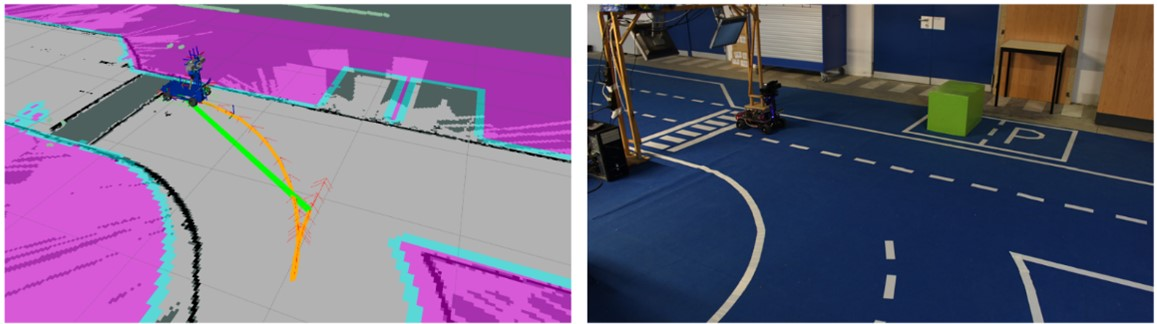
\includegraphics[width=.8\linewidth]{img/auto_1.jpg}
  \caption{後退動作}
  \label{auto:comp:koutai}
  \end{center}
\end{figure}

\subsection{Driverless Carのデザインと実装:三重県南伊勢町における実証実験}
浦瀬ら\cite{auto:design}は、Last One Mile において利用者が自在に移動できるようにする
Driverless Car のデザインと設計・実装について、歩行者空間も走れるような自律走行車両をLast One Mileにおいて提供する、
設計コンセプトの実証を行った。三重県南伊勢町で行われたフィールドワークをもとにDriverless Carのコンセプトを設計し、
設計したコンセプトから実装を行い、これを用いて、南伊勢町における実証実験を行い、その有効性を実証した。
文献では、LiDARセンサとIMUを用いたパーソナルビークルの自律移動システムを開発している。
ここでは、プロトタイプの開発として、1/10スケールのRCカーを用いた手動走行、地図作成、自己位置推定、経路計画のシステムを構築している。
AMCLによる自己位置推定が実装されており、環境地図を用いた位置推定の精度を評価している。
椅子やゴミ箱などの物体が存在する環境で、地図に特徴のあるエリアでは、自己位置の推定精度が高く、平坦で長い廊下等の特徴量の少ない経路では、自己位置推定の精度が下がる結果が報告されている。
しかし、自己位置推定の実装では環境地図中での手動動作におけるAMCLの精度のみを評価しており、RCカーの自律移動の精度に関しては、評価が行われていない。
また、車型の自律移動特有の切り返し動作においても、同様であったかは、不明である。

\section{提案}
これまでの記述により、自律移動ロボットは、センサ数を少なくする方針で設計されている。
また、4輪車両型の自律移動システムにおいては、比較的少ないセンサ数でのシステム評価、特に、LiDARのみによるSLAM、ナビゲーションシステムの評価は行われていない。
LiDARとイメージセンサ等によるセンサフュージョン技術による駐車や車庫入れのような複数の移動の組み合わせの評価は行われているが、LiDARのみによる自律移動を実現することが理想と考えられる。
LiDARのみによる自律移動が実現できれば、制作コストの削減や、保守性の向上が期待される。

そこで、本研究では、遠隔操作と自律移動の機能の切り替え機能を有する、自動運転システムを提案する。
遠隔操作機能として、車載カメラ映像をモニタで確認しながら、ハンドル・フットペダルゲームコントローラの入出力によってRCカーの遠隔操作を実現する。
遠隔操作の際には、LiDAR SLAMによる環境地図を作成し、プログラムを切り替えることで、作成した環境地図中の自律移動を実現する。
自動運転機能の評価として、自動運転から手動運転への切り替え機能の評価と、後退機能と旋回機能を組み合わせた、切り返しの機能の検証を行う。

\subsection{システム構成}
以下と、図\ref{auto:system}に、本研究で使用するハードウェアとソフトウェアとシステム全体の構成を示す。
\begin{enumerate}
  \item ハードウェア\\
  Arduino、Raspberry Pi 4 model B、URG-04LX-UG01、モータドライバ(pca9685)、ノートPC
  \item ソフトウェア\\
  Ubuntu 18.04 LTS(OS)、ROS Melodic
\end{enumerate}

\begin{figure}[h]
  \begin{center}
  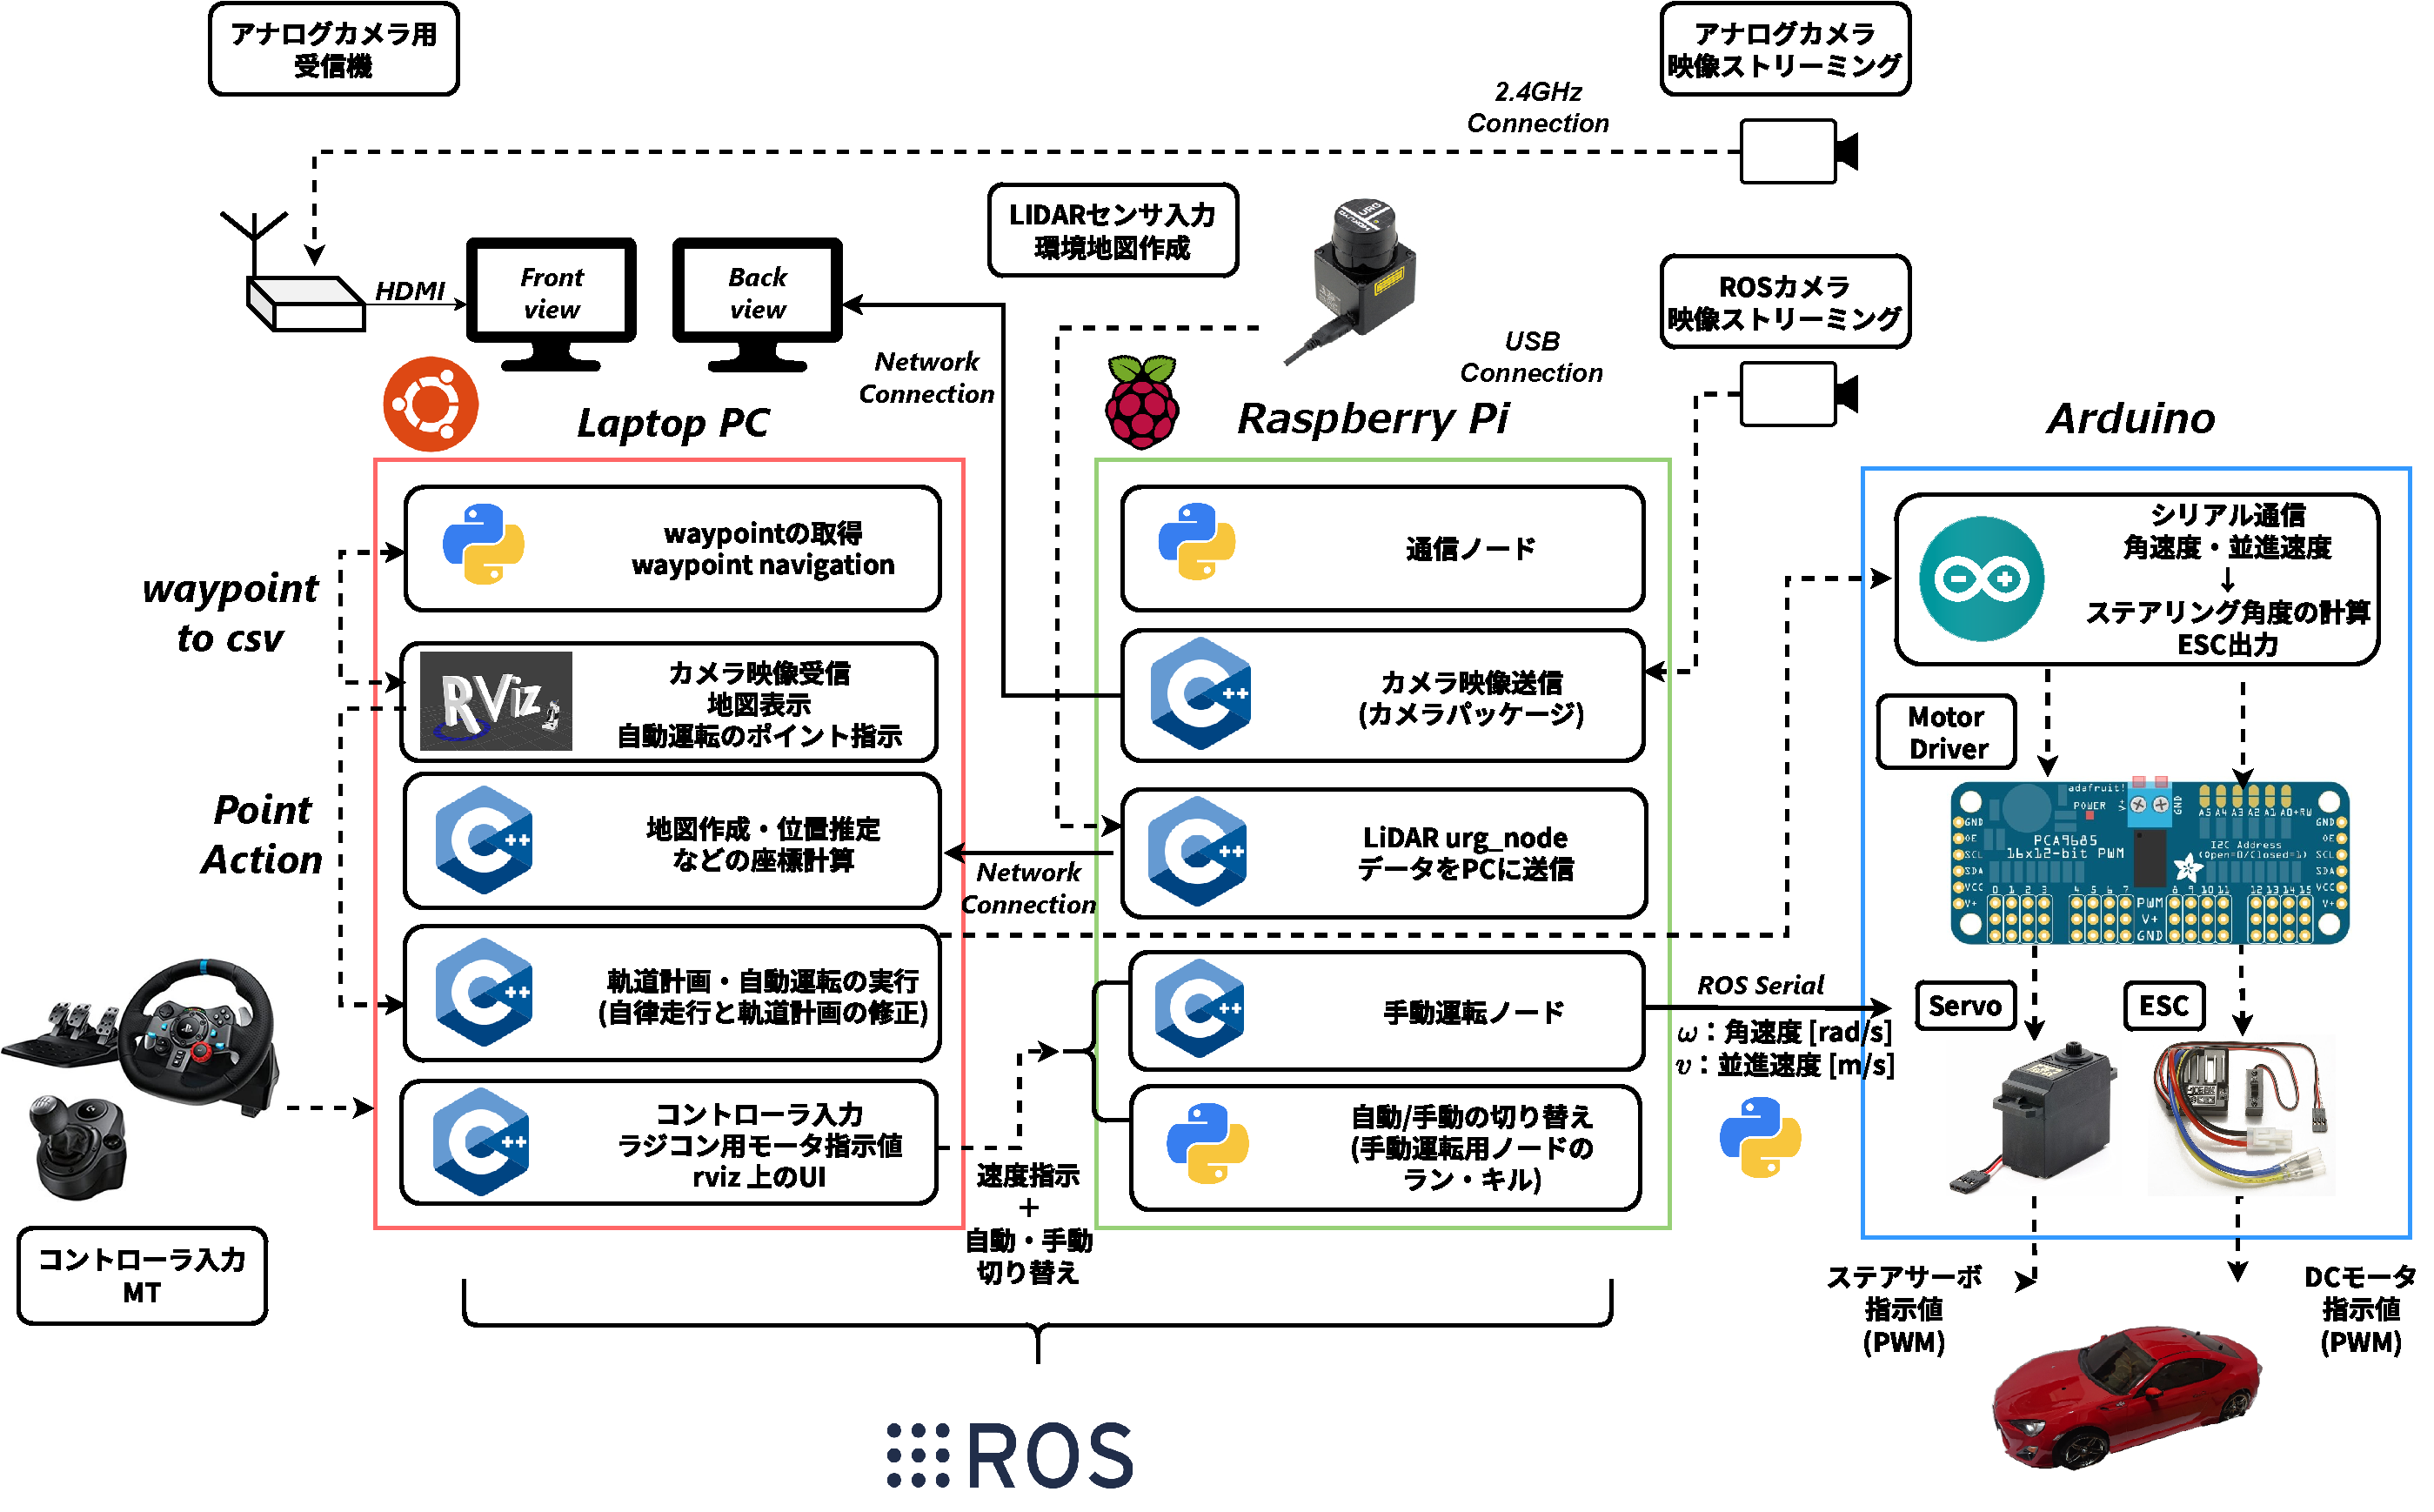
\includegraphics[width=\linewidth]{img/auto_2.pdf}
  \caption{システム構成}
  \label{auto:system}
  \end{center}
\end{figure}

\subsection{システムインターフェース}
\subsubsection{ステアリングコントローラによる遠隔操作}
ステアリングコントローラの入力に対するRCカー動作について、ハンドルフットペダルによるモータ制御を図\ref{auto:servopwm}、\ref{auto:dcpwm}に示す。
ハンドル部分の回転角値(アナログ値)をRCカーの角速度値に変換し、その後さらにサーボモータの制御パルス値に変換し、サーボモータに出力する。サーボモータに連動して、ステアリング機構が駆動する。
アクセルペダル部の踏み込み値(アナログ入力)を並進速度値に変換し、その後モータドライバの入力値(DCモータの制御パルス値)に変換し、DCモータに出力する。
DCモータに連動して、タイヤ部が回転することで前進・後退動作を実現する。
ブレーキペダルを踏みこむことでDCモータの停止値が出力され、タイヤの駆動が停止する。
ステアリングコントローラのハンドル部とペダル部に回転角を検出するセンサが搭載されている。
それぞれのセンサが示す入力値を解析することができれば、入力値に対応させた電圧パルス値の制御の処理を行うことができる。
解析したセンサの入力値をRCカー側のコンピュータへと送信し、RCカーの制御用マイコンがRCカーを制御する。
Wi-Fiによる無線通信をノートPCとRCカー側のコンピュータで行う。
制御信号の伝送をRCカー側のコンピュータとマイコンのシリアル通信により行う。
ノートPCがステアリングコントローラの入力値を解析して角速度と並進速度値に変換し、Wi-Fi経由でRCカー側のコンピュータに送信する。
RCカー側のコンピュータが、並進速度値と、角速度値をシリアルポート上に送信する。
マイコンが並進速度値と角速度値を受信し、モータの制御パルス値に変換することで、RCカーを動作させる。
また、本研究では、AT(Automatic Transmission)の他に、MT(Manual Transmission)による操作を行う。
前進・後退動作を行う際、MT操作のパドルシフトとして、ステアリングコントローラに搭載された2つのパドルスイッチの入力により、シフトアップとシフトダウンを行うことで、モータの回転速度値を変更する機能を実現する。
加えて、MT操作のHパターンシフトとして、クラッチペダルとシフトレバーの両方の入力を検知することで、RCカーの前進速度の変速と、前進・後退のモード切り替えを行う。
\begin{figure}[h]
  \begin{center}
    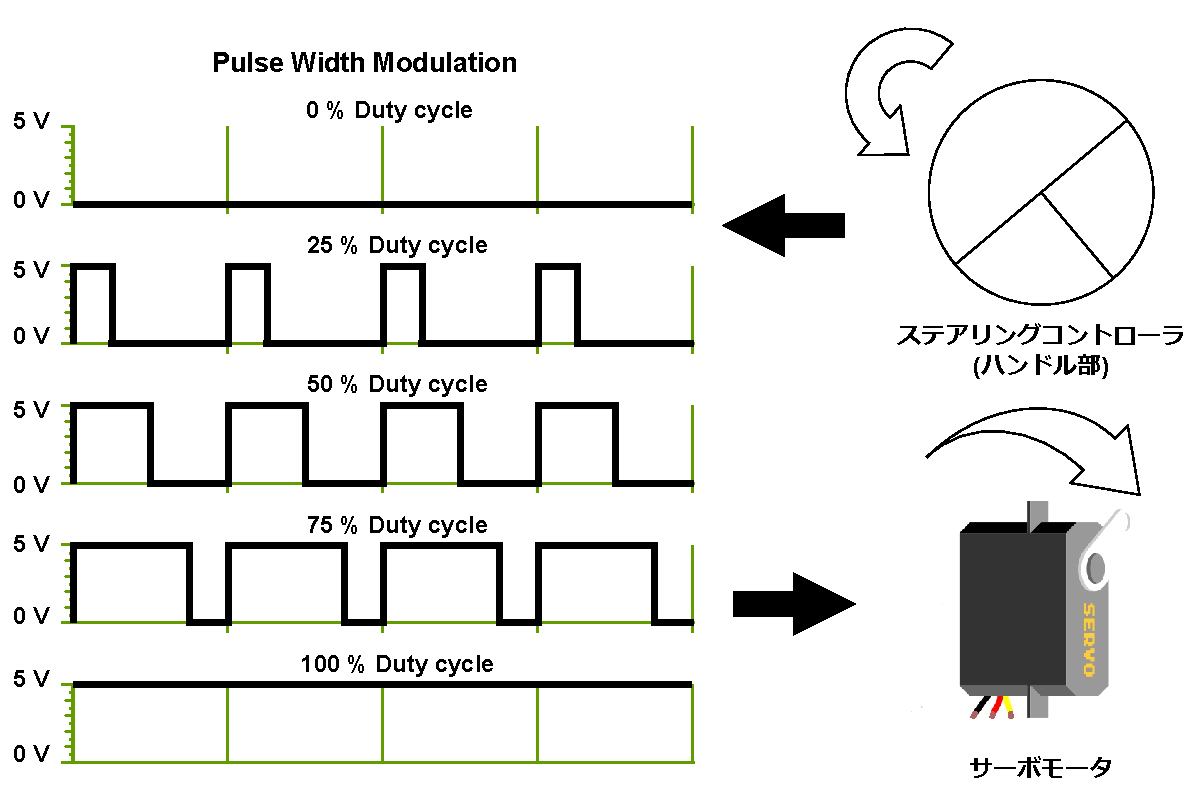
\includegraphics[width=.75\linewidth]{img/auto_3.pdf}
    \caption{ハンドルによるサーボモータの制御パルス値の取得}
    \label{auto:servopwm}
  \end{center}
\end{figure}

\begin{figure}[h]
  \begin{center}
    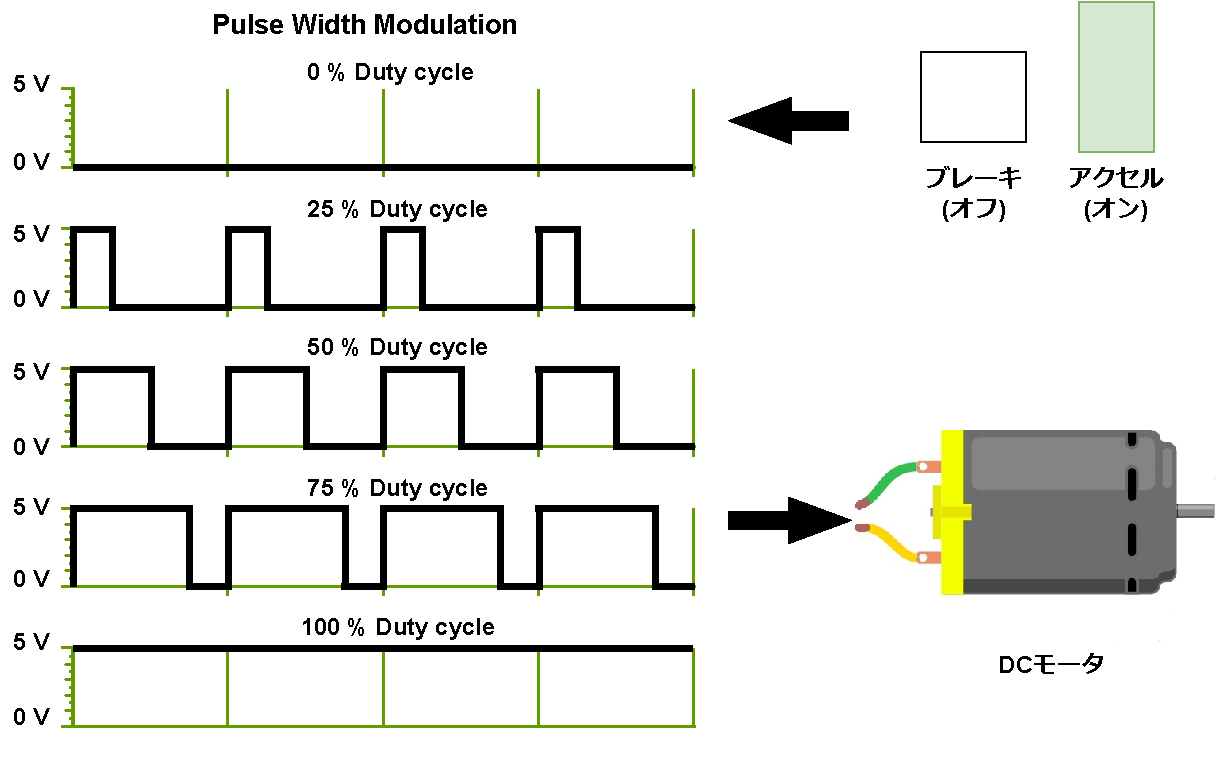
\includegraphics[width=.75\linewidth]{img/auto_4.pdf}
    \caption{ペダルによるDCモータの制御パルス値の取得}
    \label{auto:dcpwm}
  \end{center}
\end{figure}


\subsubsection{カメラ映像の取得}
RCカーの遠隔操作で、車両側周囲の状況を把握するためにカメラ映像をリアルタイムで送信するシステムを導入する。
RCカー側に取り付けられたカメラの映像をWi-Fiや、高周波帯の電波により運転者側に送信し、受信した後に、ディスプレイに出力する。

\subsubsection{SLAM}
RCカーにLiDARセンサを搭載し、LiDARによって取得した、点群データを用いて環境認識を行う。環境認識によって、RCカーの自己位置の推定と、
RCカーが走行した周辺の環境地図の構築を行う。LiDARは、RCカー側に搭載したコンピュータに接続し、点群データをWi-Fi通信により、ノートPCへと送信する。
また、自己位置・地図構築に関する計算は、ノートPCで行う。全体の流れとして、SLAMと遠隔操作のプログラムを同時に起動し、
環境地図を取得する。取得した地図は、ファイル形式を指定して保存をする。

\subsubsection{自動運転機能}
SLAMによって取得した地図を読み込み、地図中でRCカーの初期位置を設定し、目的地点を設定すると、目的地点の座標と、初期位置の座標、
地図情報(障害物の位置)等から、最適な経路計画を行う。経路計画に基づいて、並進速度と、角速度を出力し、その値をモータの制御パルス値に変換して出力する。

\subsubsection{waypointの設定}
環境地図の座標系を下に、自律移動の目的地をコースの形状に沿って複数の点に分割して設定した中継地点をwaypointと呼ぶ。
図にwaypointの例を示す。周回コースに設定したwaypointに到着すると、次のwaypointへと自律移動を開始する。設定したwaypointにはマージンを設定し、waypointから
半径数\si{[m]}程度の閾値を設定し、ロボットが閾値以内に到着すると、次の設定点への経路計画を行う。

\subsubsection{自動運転・手動運転の引継ぎ機能}
AMCLによる自己位置推定をしながら、環境地図中を遠隔操作し、地図中の経路の途中でコントローラのボタンを
入力すると、遠隔操作のプログラムが終了し、自律移動のプログラムが起動する。自律移動のプログラムが起動している最中に、
もう一度コントローラのボタンを入力すると自律移動のプログラムが終了し、遠隔操作のプログラムが再び起動する。

\section{実装}

\subsection{システムの実装}
システムのハードウェアが行う機能を以下に示す。

\begin{enumerate}
  \item Arduiono:Raspberry Piとのシリアル通信、モータの制御パルスの出力、モータドライバへの入力
  \item Raspberry Pi:ノートPCとの通信(ROSマスター)、LiDARのデータとカメラ映像をPCに送信、Arduinoに並進速度と角速度のデータを送信
  \item LiDAR:Raspberry Piとのシリアル通信、環境認識・点群データの取得
  \item ノートPC:Raspberry Piとの通信(ROSスレーブ)、地図構築・経路計画の計算、経路計画・環境地図の可視化(RViz)、カメラ映像の受信
\end{enumerate}

\subsection{ROSについて}
ROS(Robot Operating System)\cite{auto:ROS}は、知能ロボットの研究開発についてのソースコードの汎用性、移植性とモジュール化への要求等の需要を満たすために、
2010年にWillow Garage社が発表したミドルウェアである。ROSのスタック構成を図\ref{auto:ros}に示す。
ROSは、ロボット開発を行うためのソフトウェアの集まりであり、プロセス間通信のためのライブラリと、プログラムをコンパイルするためのビルドシステムを提供している。
ROSの特徴として、アプリケーション側から見た時には、ハードウェアの抽象化、各種ドライバの管理、共有機能の実行管理、ジョブ管理、プロセス間のメッセージパッシングなど、基本OSの管理機能に類似する上位機能を提供しており、ロボット向けの基本OSになれるように設計されている。
本来の基本OSはROSによりカプセル化され、ロボットアプリケーションからはシームレスとなっている。
ROSの設計目標の最も重要な要素の一つは、ソースコードのユーザビリティを改善することである。
ROSは分散処理システムであり、各種ロボット向けの基本機能のうち、汎用性のある部分をノード(nodes)と呼ばれる機能モジュールに表現されている。
そして、ノードを組み合わせることにより、より複雑な制御機能を分散的に実現する。これらのノードモジュールをパッケージ(package)にまとめることができるので、開発済みの機能モジュールの共有と配布が簡単に行えるようになっている。
さらに、ROSのファイルシステムでは、統合開発環境をサポートしており、ファイルレベルからライブラリレベルまでの設計、開発、管理を独立的に行うことができる。
ROSは、分散型処理システムであり、各ノードは通信モジュール間のピアツーピアネットワークで関係づけられている。
このネットワーク上で同期型リモートプロシージャコール(remote procedure calls, RPC)を基にしたノード間の通信や、トピック(topic)の配布/購読により実現される非同期型データ通信、パラメータサーバでのパラメータ(グローバル変数)の分散的格納と取り出し機能を提供されるが、厳密なリアルタイム性を持たない。

\begin{figure}[h]
  \begin{center}
    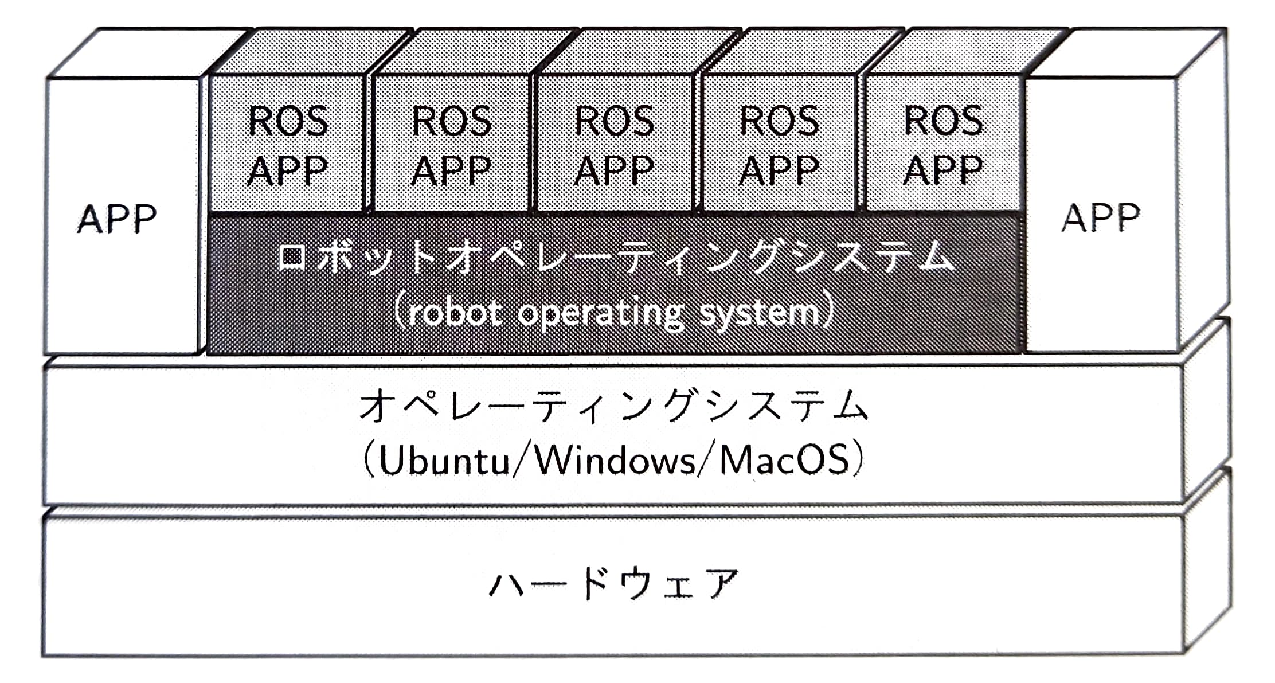
\includegraphics[width=.75\linewidth]{img/auto_5.pdf}
    \caption{ROSのスタック構成}
    \label{auto:ros}
  \end{center}
\end{figure}

\subsubsection{ピアツーピア設計方式}
ROSの実行ジョブは、分散された一連のプロセスで構成される。
図\ref{auto:rospeer}に、ROSのピアツーピア設計例を示す。
これらのプロセスは同じホスト、または、別々のホスト上に分散させることができ、プロセス間ではピアツーピアネットワークを構成する。
このようなピアツーピア設計を利用することにより、サービス管理やノード管理等を、ビジュアル処理部または音声処理部等のロボットの補助処理部から、計算負荷を分散させることができる。

\begin{figure}[h]
  \begin{center}
    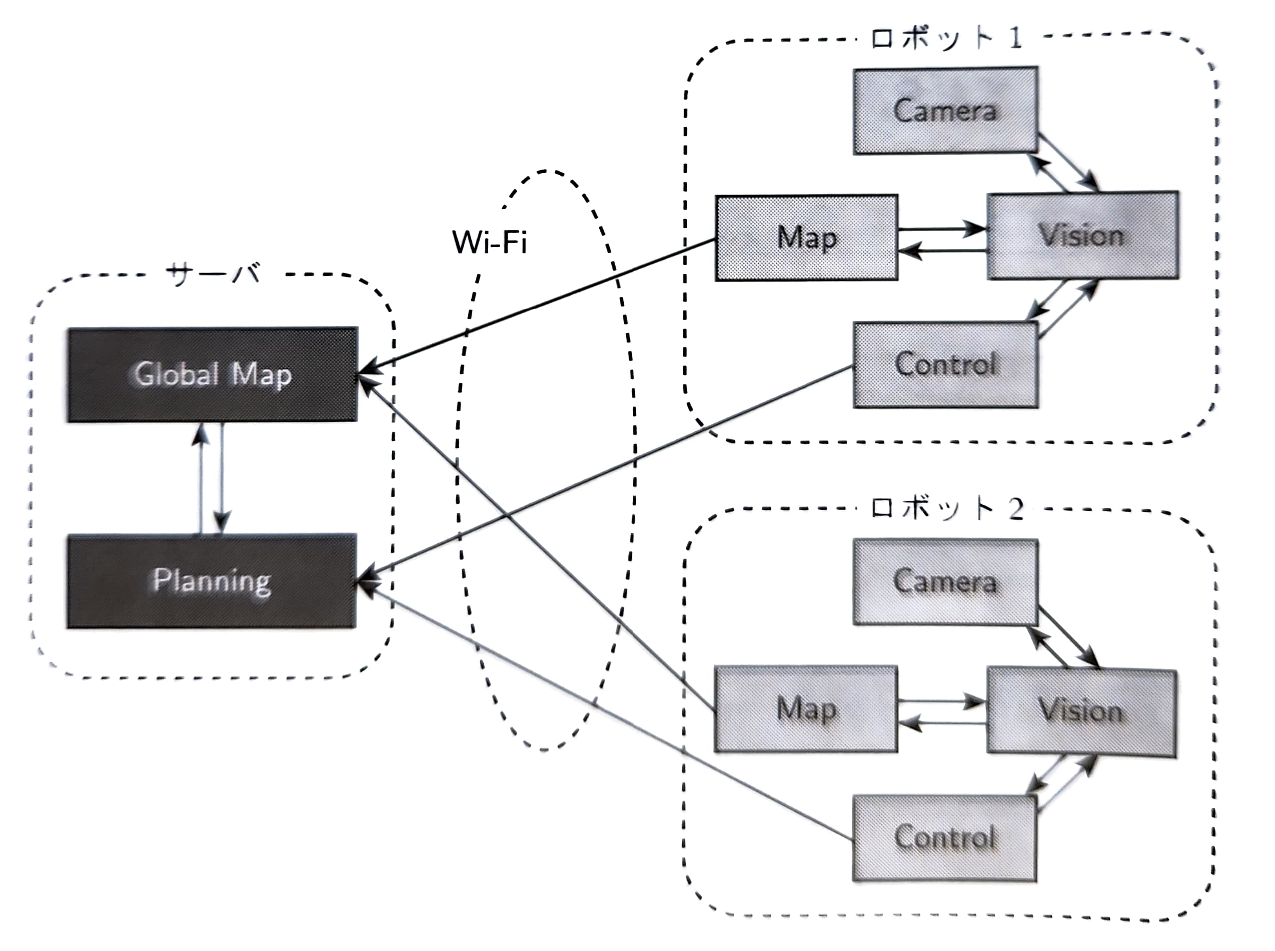
\includegraphics[width=.75\linewidth]{img/auto_6.pdf}
    \caption{ROSのピアツーピア設計例}
    \label{auto:rospeer}
  \end{center}
\end{figure}

\subsubsection{多言語に対応}
様々な開発者のニーズに対応するために、ROSでは、\verb|C++|、Python、Java等、複数のプログラミング言語をサポートしている。
複数の言語が混在する環境では、ROSはプログラミング言語に独立する簡単なインターフェース定義言語を提供し、各モジュール間でのメッセージ通信を表現する。
インターフェース定義言語で構成されるテキストファイルでは、各ノードのメッセージの構造を表現している。
これにより、オブジェクトコードを生成する際に、対応するコードをノードごとに生成することができる。

\subsubsection{機能の細分化と集約}
既存の手法で知能ロボット向けのソフトウェアを開発する場合、重複作業が多く、
本来共有すべきドライバ等のソースコードは、各ロボットのミドルウェアの正弦で抽出しにくく、他のロボットへ採用することが困難であった。
ROSの場合、汎用性のある機能、または計算処理部を独立性のあるモジュールにしており、各モジュールはCMakeにより単独にコンパイルすることができる。
さらに細分化された汎用性のある機能モジュールをライブラリに集約することにより、より複雑な機能が実現しやすくなり、ユーザビリティの改善が期待できる。

\subsubsection{補助ツールが豊富}
複雑になっていくROSパッケージを管理するために、ROSではさまざまなツールを用意して、ROSパッケージのビルド管理や、
新しい機能モジュールの開発を比較的簡単にしている。ROSのコア部は、知能ロボットを制御する基本的な部分しかもっておらず、
モジュールを追加することにより、様々なバリエーションをもたらすことができる。これらの補助ツールは、全てのロボットの共通機能を
組み合わせるために方法を提供している。

\subsubsection{オープンソースのプラットフォーム}
ROSの全てのソースコードが一般公開されており、それらのほとんどがBSDライセンスのもとで、使用できる。
つまり、非商用/商用での使用が許可されている。

\subsubsection{コンピューティンググラフ}
ROSのコンピューティンググラフはデータの処理場の依存関係を表すもので、ポイントツーポイントネットワークで示される機能グラフのことである。
ROSのコンピューティングレベルでは、ノード、マスター、パラメータサーバ、メッセージ、サービス、トピック、バッグという機能単位があり、
これらを機能的に表現することにより、ネットワークグラフが構成される。

\begin{enumerate}
  \item ノード\\
  処理機能の基本単位で、処理プロセスを表す。図\ref{auto:compute}にROSのコンピューティングレベルを示す。
  ROSでは、プロセス間のデータ通信を実現するために、各プロセスをノードで表現する必要がある。
  通常では、ROSシステムは様々なノードより提供されている機能で構成されているが、ノードの設計方針として、複雑な機能表現、あるいは、たくさんの機能を持たせるのではなく、できるだけ単一機能にする、ということがある。
  そして、このように単純化されたノードを組み合わせることにより、より複雑な機能を実現する。
  ノードはroscppやrospy等、ROSのクライアントライブラリにより生成することができる。
  \begin{figure}[h]
    \begin{center}
      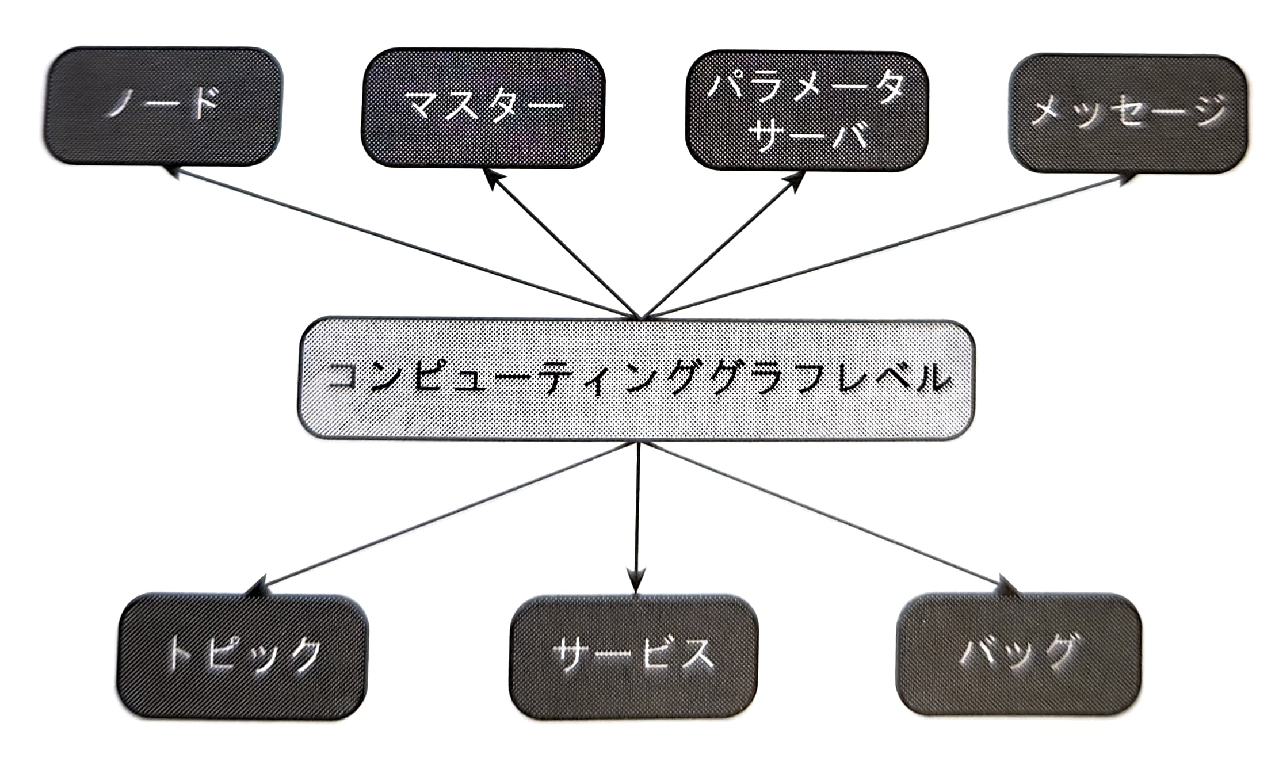
\includegraphics[width=.75\linewidth]{img/auto_7.pdf}
      \caption{ROSのコンピューティングレベル}
      \label{auto:compute}
    \end{center}
  \end{figure}
  \item マスター\\
  ROSのノードやトピック、サービスの管理を行う機能単位である。
  ROSシステムの中でマスターが起動していなければ、ノード間の通信ができない。
  マスターを利用すれば、異なるコンピュータの中のノード間の通信も実現することができる。
  マスターの仕組みは、roscoreというプロセスにより提供されている。
  roscoreは、ノードやトピック、サービスなどの名前の登録、ノードのURIの検索、トピックの検索、トピックに対する購読者の参加通知等を提供する。
  ROSシステムの中で、roscoreは必ず一つ立ち上げておく必要がある。
  \item パラメータサーバ\\
  ROSにはトピックの他に、数値等のデータを送受信する仕組みとしてパラメータ通信機構がある。
  パラメータは、パラメータサーバにグローバル変数として保持しておくことができる。
  パラメータは本来、ノードをコンフィグレーションする目的で利用される。
  パラメータサーバを利用すれば、ほかのノードと協調しながらノードのダイナミックコンフィグレーションを実現することができる。
  \item メッセージ\\
  前述のとおり、ノード間で通信を行うデータ単位の一つであり、様々なデータタイプを持つ。
  \item トピック\\
  ROSネットワーク中で転送される各メッセージは識別子を持つ必要がある。図\ref{auto:kyoyu}にROSトピックを利用した情報共有を示す。
  配布者が提供するデータは、トピックの形でROSネットワーク中に公開される。
  購読者は、自分の関係にあるトピックを常に監視していて、自分のメッセージタイプでトピックのデータを受け取って利用する。
  つまり、トピックはメッセージのインスタンスであると考えてよい。メッセージのインスタンスを生成する側は配布者、利用する側は購読者である。
  例えば、カメラ映像で取得した画像を利用する複数のノードがあるとすると、カメラノードは画像メッセージをトピックとして発行し、他のノードはそのトピックを監視して、カメラ情報を分散的に利用することができる。
  なお、トピック名は、ROSシステム中で動作しているノード間での唯一性を保証する必要がある。
  \begin{figure}[h]
    \begin{center}
      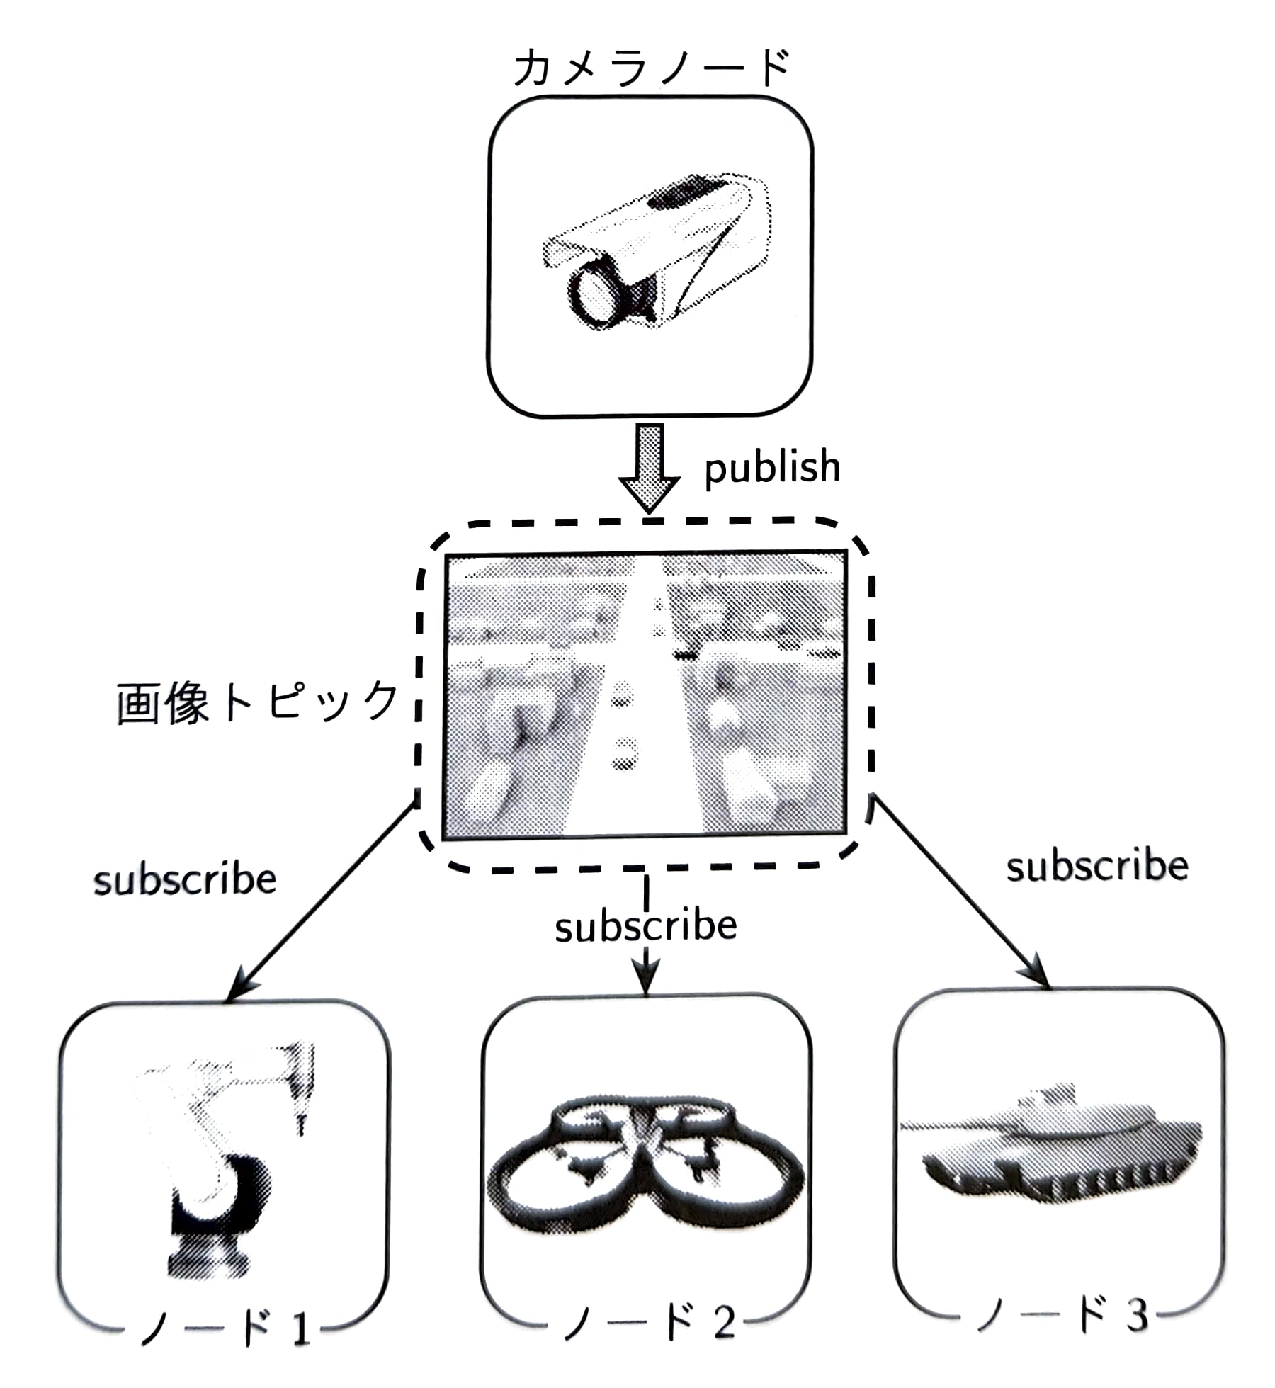
\includegraphics[width=.8\linewidth]{img/auto_8.pdf}
      \caption{トピックを利用した情報共有}
      \label{auto:kyoyu}
    \end{center}
  \end{figure}
  \item サービス\\
  ノード間で通信を行うための一つの手段である。サービスは、ROSネットワークの中でただ一つの名前で識別される。
  \item バッグ\\
  ROSメッセージの記録と再生に使われる。バッグは、収集しにくいセンサデータを処理するアルゴリズムを開発・テストする際に、
  データを収納する重要なメカニズムであり、複雑なロボットを制御するロボットのプログラムを開発する際に大変重要な役割を果たす。
\end{enumerate}

\clearpage

\subsection{遠隔操作機能の実装}
\subsubsection{コントローラ入力値解析}
ステアリングコントローラはゲーム用のコントローラや、ジョイスティック全般と共に、
ROSのjoyパッケージを用いて、解析を行う。joyパッケージは、ゲーム用のコントローラのボタン全てにディジタル入力とアナログ入力を与える。

\subsubsection{ステアリング・前進後退機能(AT・MT)}
コントローラ入力値解析によって、得られた入力値のうち、ハンドル入力値を角速度(単位:\si{[rad/s]})の値に変換する。
アクセル・フットペダルの入力値を並進速度(単位:\si{[m/s]})の値に変化する。
なお、角速度、並進速度等のトピック通信には、ROSの定義済みメッセージタイプである\verb|geometry_msg(float32)|を用いている。

\subsubsection{ROSマスタースレーブ(Laptop to Raspberry Pi)}
ROSシステム内の全てのホストは、互いに到達できることが要求される。それぞれのホストは同じネットワークに所属しなくても良いが、ルータ等を経由して
必ずたどりつけるようにしなければならない。(DNSなどでIPアドレスが解決できることと、宛先への経路が確保できる)ROSシステムのホスト(マスター)をRaspberry Piに、
スレーブをノートPCに設定する。設定は、ROSシステムのホストを決める環境変数にマスターとするマシンのIPアドレスを登録すれば、
プログラム起動時に自動的にマスターを検索して接続する。

\subsubsection{シリアル通信(Raspberry Pi to Arduino)}
Raspberry PiとArduino間の通信として、ROSのシリアル通信用パッケージrosserialを用いる。rosserialは、
主に、pythonノードや、Arduinoをクライアントとすることを前提とされており、シリアルポート、ボードレート等を指定し、通信ノードとして起動させることで、
ホストとクライアント間でトピック通信を行うことができる。

また、Arduino側に\verb|ros_lib|APIを用いることで、ArduinoがROSのシリアルクライアントとしてROSのマシンとトピックの通信を行うことができる。

\subsubsection{カメラ映像機能}
カメラ映像には、5.8 \si{[GHz]}電波帯とVTX(Video Transmitter)を用いることで、リアルタイム映像を受信することができる。また、ROS側でも、USBカメラをRaspberry Piに接続することで、可視化ツール
RViz上に映像を送信する。

\subsection{SLAMの実装}

\subsubsection{urg node}
北陽電機社製のLiDARは、北陽電機株式会社が開発した\verb|C++|ドライバソフトウェアurg\verb|_|nodeをROS環境にインストールすることで
点群データの取得に使用できる。urg\verb|_|nodeで使用するシリアルポート、検知角度等のパラメータを設定する。

\subsubsection{Gmapping}
ROSで既に実装されているSLAMメタパッケージの1つとして、Gmappingが挙げられる。Gmappingは、LiDARのデータとオドメトリ情報(必須)
を用いてSLAMを行う。ROSを用いたSLAMで最も多く使用されているパッケージである。

\subsubsection{laser scan matcher}
今回の開発では、ロータリーエンコーダや、IMU等の内界センサを用いないため、Gmappingパッケージを用いるための内界センサ以外からのオドメトリ情報が必要である。
その一つとして、レーザオドメトリを使用する。レーザオドメトリとして、LiDARのスキャンデータの差分から、オドメトリデータを生成する\verb|laser_scan_matcher|パッケージを用いる。

\subsection{自動運転機能の実装}
自動運転機能は、GmappingによるSLAMで生成された地図上の経路計画を行うNavigation Stack\cite{auto:navstack}と、自己位置推定を行うAMCL\cite{auto:amcl}を用いる。
以下にNavigation StackとAMCLについて述べる。

\subsubsection{Navigation Stack}
ROSでは、自律移動を目的としたメタパッケージNavigation Stack\cite{auto:navstack}が構成されている。
図\ref{auto:navstack:state}にNavigation Stackの概要を示す。
Navigation Stackとは、オドメトリ情報(ホイールエンコーダ等の内界センサによる推定自己位置及び現在速度)、および、LiDARの情報(障害物までの距離情報)を入力値として、与えられた目標地点/姿勢に到達するための安全な駆動(速度)命令を出力するソフトウェアである。
LiDARの情報は、平面レーザによる2Dレーザスキャンまたは3Dデプスカメラ等によるポイントクラウドを利用可能である。
Navigation Stackを扱うためには、TF(Transform tree)と呼ばれる座標軸の相対位置情報を与える必要があり、オプションで、Navigation Stackに対して地図を与えることができる。
地図を与えることで、Navigation Stackはより効率的に移動経路の探索を行うことができる。

\begin{figure}[h]
  \begin{center}
    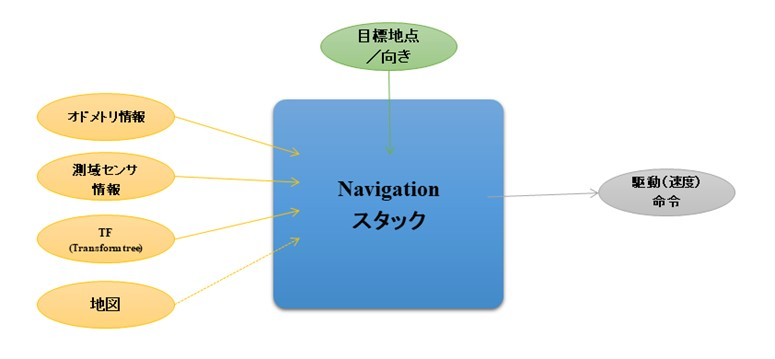
\includegraphics[width=.6\linewidth]{img/auto_9.jpg}
    \caption{Navigation Stackの概要}
    \label{auto:navstack:state}
  \end{center}
\end{figure}

\subsubsection{Transform Tree}
Transform Tree(tf)とは、ロボットが存在する空間及びロットの構成要素がそれぞれ持っている座標軸ごとのずれ
(x,y,zの相対位置及び相対姿勢)がどの程度であるかを、親子関係のツリー構造で表現したものである。例えば、
障害物からの距離情報は、ロボット上に設置されたレーザから取得されるが、ロボットの障害物回避を考える場合は、ロボットの基準面の位置で考える必要がある。
これを求めるために、基準面の座標軸とレーザ座標軸とのずれをNavigation Stackに入力する必要がある。

\begin{figure}[h]
  \begin{center}
    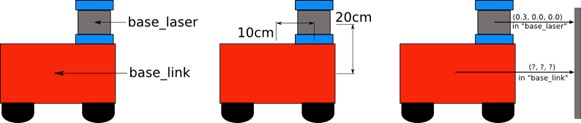
\includegraphics[width=.8\linewidth]{img/auto_10.jpg}
    \caption{Transform Treeの説明}
    \label{auto:navstack:tf}
  \end{center}
\end{figure}

各座標軸は、\verb|frame_id|と呼ばれる文字列により識別される。Navigation Stackが動作するには、基本的な構成の場合は、
mapフレーム、odomフレーム、base\verb|_|linkフレーム、laserフレームの4つの構成要素の相対位置・姿勢(3つのTransform Tree情報)が必要である。
mapフレームは、Transform Treeの頂点座標軸で、ロボットが移動する空間で固定となる絶対座標系である。
odomフレームは、ロボットのオドメトリ(内界センサーによる推定自己位置)を表すための座標軸である。
mapフレームと同じ空間固定座標軸であり、車輪の空転やロボットの横滑り、オドメトリの計算誤差がないならば、mapフレームとのずれは理論上常にゼロとなる。
(実際には計算誤差やスリップ等があるため、mapフレームとのずれは時間と共に拡大していく。) base\verb|_|linkフレームは、ロボット基準面の中心を原点とする座標軸である。
ロボットの移動に伴い、odomフレームとの相対位置・姿勢が変化していく。
laserフレームは、ロボット上のLiDARの基準点を原点とする座標軸である。
一般的には、LiDARはロボット上に固定されるため、base\verb|_|linkフレームとの相対位置・姿勢は固定値となる。

\begin{enumerate}
  \item LiDAR情報(レーザスキャン)\\
  レーザスキャンデータは、laser座標系における、スキャン範囲内の各スキャン谷における、障害物までの距離を通知する。
  図\ref{auto:navstack:laser_scan}にレーザスキャンのパラメータ値を示す。  例えば、測定範囲が180度で、測定単位が5度のレーザセンサであれば、36個の距離データ(ranges)を通知する。
  測定範囲内に何もない部分については、無効値(range\verb|_|max値または無限大)を入れておく。
  測定角度は、前方正面が0ラジアンで、右側がマイナス値、左側がプラス値となる。
  \begin{figure}[h]
    \begin{center}
      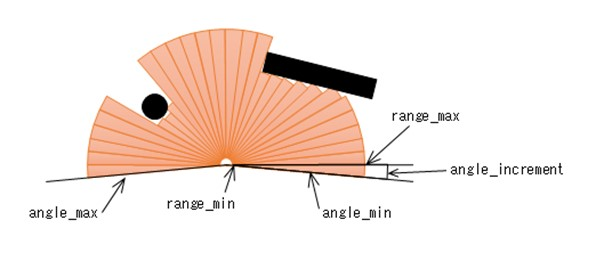
\includegraphics[width=.8\linewidth]{img/auto_11.jpg}
      \caption{レーザスキャンのパラメータ値}
      \label{auto:navstack:laser_scan}
    \end{center}
  \end{figure}

  \item オドメトリ情報\\
  オドメトリ情報は、odom座標軸におけるロボット(base\verb|_|link座標系)の推定自己位置及び現在速度(並進速度および回転速度)を通知する。
  図\ref{auto:navstack:odometry}にオドメトリの座標系を示す。推定自己位置は、多くの場合、車輪駆動を制御するノードが、車輪回転量から推定される自己位置情報を通知する。
  (IMU等、車輪回転量とは別の何等かの手段を組み合わせて、オドメトリ情報の精度を上げることも可能である。)
  現在速度は、2Dのナビゲーションでは、x軸並進速度及びz軸回転速度が設定される。
  座標系の考え方は、下図の通りで、ロボット前方がx軸正方向、ロボット左方向がy軸正方向となる。
  z軸回転速度は、左回転が正方向である。
  \begin{figure}[h]
    \begin{center}
      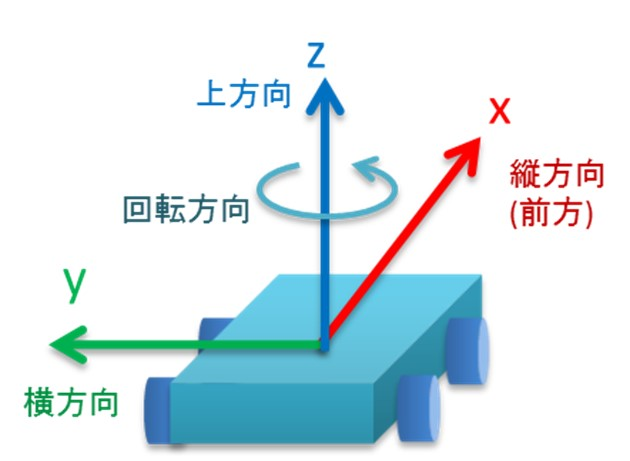
\includegraphics[width=.8\linewidth]{img/auto_12.jpg}
      \caption{オドメトリの座標系}
      \label{auto:navstack:odometry}
    \end{center}
  \end{figure}
  odomとbase\verb|_|linkの相対位置については、TFでも同じ内容が通知される。
  Navigation Stackは、TFで通知される位置情報を見ており、オドメトリ情報側の自己位置情報は、
  実際には参照されていない。位置・姿勢の共分散については、x,y,z軸位置およびx,y,z軸姿勢の6つの要素について、
  推定値と実際の値との掛け合わせの相関関係を、6x6の行列データとして設定する。速度の共分散についても、同様に、x,y,z軸並進速度およびx,y,z軸回転速度の6つの要素について、推定値と実際の値の掛け合わせの相関関係を、
  6x6の行列データとして設定する。
  \item 地図\\
  オプションとして、Navigaton Stackに地図を与えることで、LiDARで見えていない後方や遠方、死角の情報も加味して経路検索を行うことができる。
  地図は、OccupancyGridというデータ形式で表現される。5cm四方など、決まったサイズのセルで地図を区切り、各セルを「占有されたセル(100)」、「占有されていないセル(0)」、「未知のセル(-1)」
  の3つで区分して地図を表現する。地図情報は、解像度(セルの大きさ)、地図の大きさ(縦横のセル数)、オリジナル(map座標系におけるセル(0,0)の位置)、その一つとして
  各セルの占有率を保持した配列データからなる。
  \begin{figure}[h]
    \begin{center}
      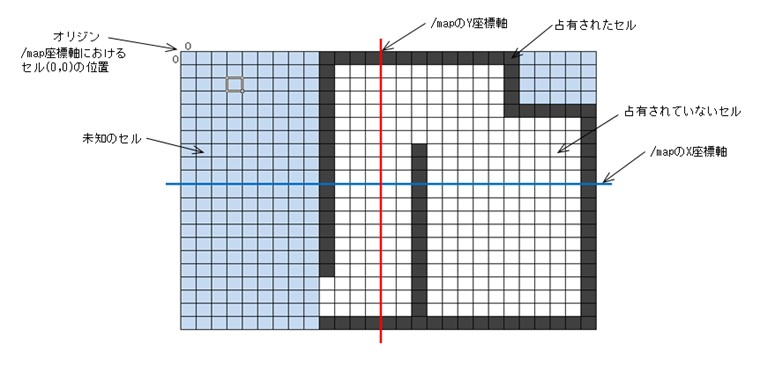
\includegraphics[width=\linewidth]{img/auto_13.jpg}
      \caption{占有格子地図}
      \label{auto:navstack:senyumap}
    \end{center}
  \end{figure}
  \item 駆動(速度)命令\\
  安全な経路を検索した結果として、Navigation Stackから駆動命令が出力される。速度は、並進速度(x,y,z)および回転速度
  (x,y,z)で表現され、一般的な2輪差動型のロボットの場合は、x軸並進速度とz軸回転速度のみ指定される。
  座標系の考え方は、オドメトリ情報の現在速度と同じである。
  \item MoveBaseアクション\\
  Navigation Stackへ、目標位置・姿勢を指定してロボットの移動を指示し、フィードバック(現在位置)および結果を受け取る。
  \item AMCL\\
  AMCL(Adaptive Monte Carlo Localization)は、2Dで移動するロボットのための確率的な位置推定システムでる。
  パーティクルフィルタ(またはKLDサンプリング)を使用したモンテカルロ法を用いて、既知のマップに対するロボットの姿勢の追跡を行う。
  \item パーティクルフィルタ\\
  パーティクルフィルタは、逐次モンテカルロ法とも呼ばれ、逐次ベイズ推定の一種で、現在の状態から想定される多数の次状態を、多数(数百か数千)のパーティクルに見立て、
  全パーティクルの尤度に基づいた重み付き平均を次状態として予測しながら追跡を行っていくアルゴリズムである。パーティクルの移動の予測や外れてしまったパーティクルの
  リサンプリングを行うことで、ガウス性のないノイズにも強い手法となっている。パーティクルフィルタは基本的に以下3つのサイクルを繰り返し実行することで推定を行う。
  予測を何回か行うごとにリサンプリングを行う。
\end{enumerate}
\subsubsection{パーティクルフィルタについて}
  \begin{enumerate}
    \item 予測\\
    図\ref{auto:navstack:predict}に、パーティクルを用いた予測を示す。
    動作モデルから求めた運動量を基に、それぞれのパーティクルを次のタイミングのパーティクルの位置に移動させる。
    各パーティクルで任意のノイズを仮定して、もとあった領域よりも広い領域に粒子をばら撒く。
    各パーティクルは、「運動モデルによって想定されるロボットの位置」という状態値の仮説を表している。
    \begin{figure}[h]
      \begin{center}
        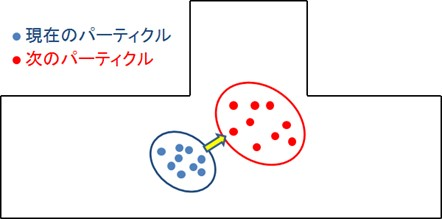
\includegraphics[width=.5\linewidth]{img/auto_14.jpg}
        \caption{パーティクルを用いた予測}
        \label{auto:navstack:predict}
      \end{center}
    \end{figure}
    \item 尤度の計算\\
    観測データにより、各パーティクルにおける尤度を計算する。図\ref{auto:navstack:yudo}に尤度の計算を示す。
    それぞれのパーティクルがどのくらい正解に近いかを観測データで決定し、実際の位置の重み付き平均やリサンプリング時の優先度等に使用する。
    レーザセンサの場合、各パーティクルでのレーザセンサの位置と壁の位置によってそのパーティクルの尤度を計算する。
    \begin{figure}[h]
      \begin{center}
        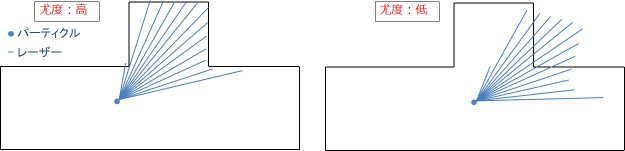
\includegraphics[width=\linewidth]{img/auto_15.jpg}
        \caption{尤度の計算}
        \label{auto:navstack:yudo}
      \end{center}
    \end{figure}
    \item リサンプリング\\
    図\ref{auto:navstack:resample}
    予測を繰り返すとパーティクルが広い領域に広がってしまうため、尤度の高いパーティクルはそのまま残して、尤度の低い
    パーティクルを尤度の高いパーティクルの周りに再配置する。全てのパーティクルを尤度の高いパーティクルの周囲に配置した場合、
    局所解に陥り、のノイズ等に対応しにくくなるため、一部パーティクルはランダムで配置する。
    \begin{figure}[h]
      \begin{center}
        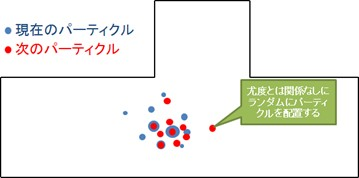
\includegraphics[width=.5\linewidth]{img/auto_16.jpg}
        \caption{リサンプリング}
        \label{auto:navstack:resample}
      \end{center}
    \end{figure}
  \end{enumerate}
  \clearpage
\subsubsection{AMCLにおけるパーティクルフィルタ}
AMCLのパーティクルフィルタの工夫について述べる。
  \begin{enumerate}
    \item オドメトリによる予測\\
    一つ前のパーティクルの位置姿勢に対し、現在のオドメトリ情報により、現在のパーティクルの位置・姿勢を予測する。
    運動モデルのタイプはdiff、omni、diff-corrected、omni-correctedの4つがある。今回は、実際に使用したdiffモデルについて述べる。
    diffモデルでは、オドメトリの並進速度に対する。各パーティクルへの回転速度・並進速度へのノイズ、オドメトリの回転速度に対する。各パーティクルへの回転速度・並進速度へのノイズが設定できる。
    前後にのみ移動するロボットに対するモデルになっている。具体的な計算方法は以下のようになる。
    \begin{enumerate}
      \item 前回のAMCLでのヨー角に対する現在のオドメトリの移動方向の角度の差分を始点角度差分とする。
      \item オドメトリの移動方向の角度と現在のオドメトリの回転速度の差分を終点角度差分とする。
      \item 始点角度差分・終点角度差分・並進速度に対してガウシアンノイズを追加する。
      \item 各パーティクルにおいて、パーティクルのヨー角に始点角度差分を足した角度を移動方向とする。
      \item 移動方向に対して並進速度の移動量を足して、現在のパーティクルの位置姿勢を求める。
      \begin{figure}[h]
        \begin{center}
          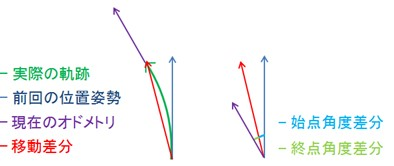
\includegraphics[width=.6\linewidth]{img/auto_17.jpg}
          \caption{diffモデル}
          \label{auto:navstack:diff}
        \end{center}
      \end{figure}
    \end{enumerate}
    \item レーザによる尤度計算\\
    外れたパーティクルの尤度が低すぎる場合は、リサンプリング時に外れたパーティクルが削除されすぎるため、パーティクルフィルタの安定性がなくなる。
    そのため、ガウシアンモデル以外のノイズも用いてレーザの値が壁と離れている場合でも尤度を持たせている。
    amclではレーザの尤度計算にビームモデルと尤度モデルを用いた推定の2種類が選択できる。
    ビームモデルと尤度モデルについて説明を行う。ビームモデルでは、「ガウシアンノイズ」と「障害物対策ノイズ」「ランダムノイズ」の組み合わせで使用している。
    それぞれのパーティクルの位置で各レーザ方向に伸ばしていき、マップ上で壁に当たる距離を計算し、その距離と実際のレンジの値によって尤度を計算する。
    そのレーザが返ってくると期待される値によって尤度を求めていく。壁に当たる位置はレーザごとに異なるため、「パーティクル数」$\times$「レーザ数」分、マップ上で壁に当たる位置を計算する必要がある。
    ガウシアンノイズは、マップ上で壁に当たる距離(レーザで期待される値)の周辺では尤度が高くなるようになる。
    \begin{figure}[h]
      \begin{center}
        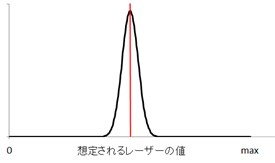
\includegraphics[width=.6\linewidth]{img/auto_18.jpg}
        \caption{ガウシアンノイズモデル}
        \label{auto:navstack:gaussnoise}
      \end{center}
    \end{figure}
    障害物対策ノイズは、地図上のレーザが当たる地点より前に、
    地図にない障害物がありレンジの値が小さくなる場合がある。その際の尤度を大きくするため、障害物対策のノイズでは、想定されるレンジより小さな値に尤度を少し上げるようなノイズを追加する。
    \begin{figure}[h]
      \begin{center}
        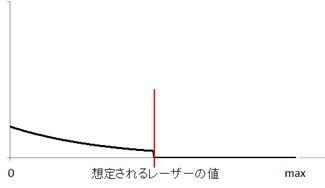
\includegraphics[width=.6\linewidth]{img/auto_19.jpg}
        \caption{障害物対策モデル}
        \label{auto:navstack:shogai}
      \end{center}
    \end{figure}
    センサの最大距離ノイズは、乱反射等によりレーザがセンサに帰ってこなかった場合、
    レンジの距離はセンサの最大値が設定される場合がある。その際に尤度を大きくするため、
    センサの最大距離ノイズでは、センサの最大距離部分では尤度が高くなるノイズを追加する。
    \begin{figure}[h]
      \begin{center}
        \subfigure[センサの最大距離ノイズ]{
        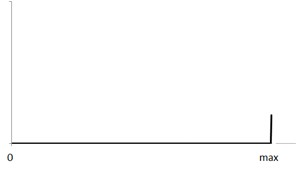
\includegraphics[width=.45\linewidth]{img/auto_20.jpg}
        \label{auto:navstack:max}
        }
        \subfigure[ランダムノイズ]{
        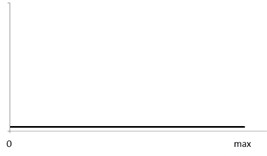
\includegraphics[width=.45\linewidth]{img/auto_21.jpg}
        \label{auto:navstack:rand}
        }
        \caption{センサノイズの分類}
        \label{auto:navstack:noise}
      \end{center}
    \end{figure}
    パーティクルフィルタで安定して動作させるため、ある程度外れてしまっているパーティクルが全て削除されることがないように、想定されるレンジの値に関わらず尤度を持たせる。ランダムノイズでは、全ての距離で一律の尤度を持たせるようなノイズを追加する。
    これらを総合した尤度のモデルは以下図\ref{auto:navstack:yugo}のようになる。各レーザに以下のモデルで尤度を計算していく。
    \begin{figure}[h]
      \begin{center}
        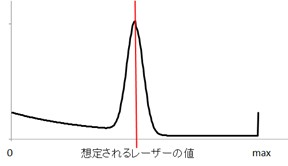
\includegraphics[width=.6\linewidth]{img/auto_22.jpg}
        \caption{融合尤度モデル}
        \label{auto:navstack:yugo}
      \end{center}
    \end{figure}
    各ノイズの重みは、パラメータにより設定できる。実行する状況に合わせてノイズの重みを変更することができる。
    各重みの和が1になるようにする必要がある。
    尤度モデルを用いたレーザは、「ガウシアンノイズ」と「ランダムノイズ」の組み合わせで使用している。マップの座標ごとにガウシアンノイズが決定するため、ビームモデルと異なり、各レーザごとに壁に当たる位置を判定する必要がなく、
    レーザの当たっている位置を求めるだけでよくなる。ガウシアンノイズは、レーザモデルとは異なり、壁からの距離で求める。
    \begin{figure}[h]
      \begin{center}
        \subfigure[ガウシアンノイズの尤度の関数]{
        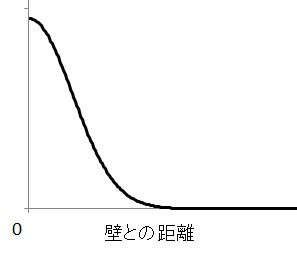
\includegraphics[width=.45\linewidth]{img/auto_23.jpg}
        \label{auto:navstack:gaussyudo}
        }
        \subfigure[ガウシアンノイズの尤度の分布]{
        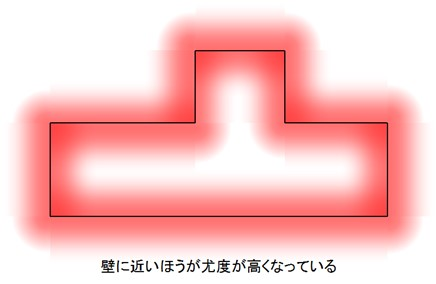
\includegraphics[width=.45\linewidth]{img/auto_24.jpg}
        \label{auto:navstack:gaussyudobunpu}
        }
        \caption{ガウシアンノイズ}
        \label{auto:navstack:gaussian_noise}
      \end{center}
    \end{figure}
    壁に近い方が、尤度が高くなる。レーザが当たった座標の尤度を使用する。
    ランダムノイズは、ビームモデルと同じで、パーティクルフィルタで安定して動作させるため、ある程度外れてしまっているパーティクルが全て削除されることがないように、想定されるレンジの値に関わらず尤度を持たせる。ランダムノイズでは、全ての距離で一律の尤度を持たせるようなノイズを追加する。
    \begin{figure}[h]
      \begin{center}
      \subfigure[ランダムノイズの尤度]{
      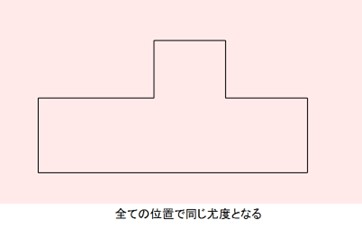
\includegraphics[width=.45\columnwidth]{img/auto_25.jpg}
      \label{auto:navstack:gaussyudorand}
      }
      \subfigure[ランダムノイズの尤度の分布]{
      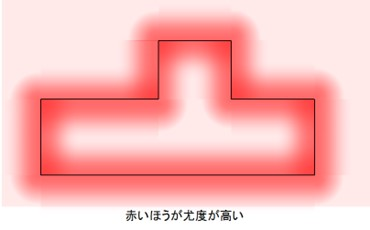
\includegraphics[width=.45\columnwidth]{img/auto_26.jpg}
      \label{auto:navstack:gaussyudorandbunpu}
      }
      \caption{ランダムノイズ}
      \label{auto:navstack:gauss_yudo_rand}
      \end{center}
    \end{figure}

    ビームモデルは各レーザに計算を行い処理に時間がかかるため、
    レーザ数・パーティクル数が多い状態でリアルタイムに実行したい場合は尤度モデルを使用するのが良い。
    また、尤度モデルでは、障害物対策ノイズ等が使用されていないため、人が多い等でマップと異なる障害物が多い場合は、ビームモデルが良いと思われる。
  \end{enumerate}

\subsubsection{Teb local planner}
\verb|teb_local_planner|\cite{auto:teb1},\cite{auto:teb2}は、前述のNavigation Stackの経路計画の内、
Timed Elastic Bandを用いた、局所計画(local planner (controller))のアルゴリズムの一つである。DWA(Dynamic Window Approach)に比べて複雑な
回避軌道を生成できるが、計算コストが比較的高いという特徴がある。計算コストを抑えつつ意図した挙動を実現するためには、
アルゴリズムを理解して、パラメータ調整を行う必要がある。

ナビゲーションモジュールにゴールが与えられると、以下のような流れを繰り返して、ゴールまでの移動を実現する。
\verb|teb_local_planner|は、軌道計画と速度・角速度制御を扱う。
\begin{enumerate}
  \item 自己位置および障害物の観測・推定
  \item 経路計画:ゴールまでの間の最適なPose列を計算する。単純な場合、ゴールが与えられるたびに一度だけ
  \item 軌道計画:ゴールまでの間の最適な各時刻のPoseを計算する。
  \item 速度・角速度制御(目標速度・角速度を計算する。)
\end{enumerate}

\begin{enumerate}
  \item Timed Elastic Band\\
  Timed Elastic Bandは、軌道を「Pose(位置と角度)の列とPose間の移動に掛かる時間の列」で表現するモデルである。
  $i$番目のPose$s_i(x_i,y_i,\beta_i)$から$i+1$ 番目のPose $s_{i+1}(x_{i+1},y_{i+1},\beta_{i+1})$ までの移動にかかる時間が$\Delta T_i$ の時、
  図\ref{auto:teb:band}に示す、TEBの模式図のように表される。
  \begin{figure}[h]
    \begin{center}
      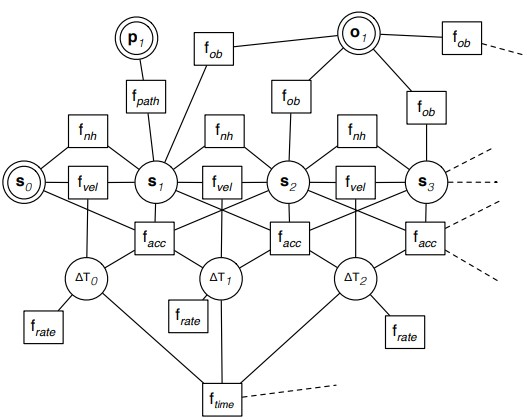
\includegraphics[width=.6\linewidth]{img/auto_27.jpg}
      \caption{TEBの模式図}
      \label{auto:teb:band}
    \end{center}
  \end{figure}
  次にTEBの最適化について述べる。
  \item 制約・目的関数\\
  \verb|teb_local_planner|は以下の制約・目的関数を満たすように最適な軌道を計算する。
  \begin{enumerate}
    \item 速度制約(2つの連続したPoseとPose間の移動にかかる時間)
    \item 加速度制約(3つの連続したPoseと2つのPose間の移動にかかる時間)
    \item 障害物/waypoint(障害物/waypointの近くの($k=3$\verb|~|$5$個の)Pose)
    \item 非ホロノミック制約
    \item 最短時間
    \item 最短距離
  \end{enumerate}
  隣接するPose間の関係によって定義される制約・目的関数は、疎行列(成分のほとんどが零である行列)で表現することができるので、
  疎行列最適化ライブラリを使用して、計算を行う。
  \item 疎行列最適化\\
  上記の制約・目的関数をHyper-Graph(エッジが複数のノードをつなぐグラフ)で表現して、g2oで最適化する。
  \begin{figure}[h]
    \begin{center}
      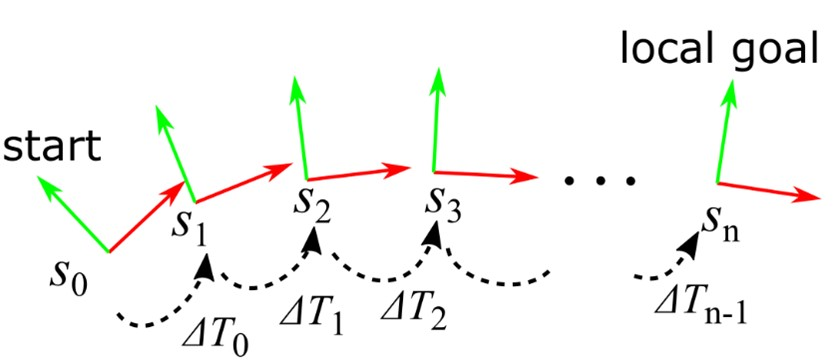
\includegraphics[width=.6\linewidth]{img/auto_28.jpg}
      \caption{疎行列最適化}
      \label{auto:teb:g2o}
    \end{center}
  \end{figure}
  図\ref{auto:teb:g2o}に疎行列最適化を示す。sはPose、pはwaypoint、oは障害物、$\Delta T$がPose間の移動に掛かる時間のノードを表している。
  これらのノードを制約・目的関数のエッジで接続することによって最適化の対象をグラフで表現する。
  \item auto resizing\\
  Timed Elastic Bandを最適化した後、サンプリング間隔が不適切になる場合がある。例としては、以下が挙げられる。
  \begin{enumerate}
    \item 障害物を回避するために経路が最適化され、サンプリングが粗くなる。
    \item ゴールが近づいて、サンプリングが過剰に細かくなる。サンプリングが粗いと軌跡の表現能力が落ち、サンプリングが過剰に細かいと計算コストがかかる。
    auto resizingは、PoseおよびPose間の移動にかかる時間を挿入したり、削除したりすることによって、この問題を解消する。以下図\ref{auto:teb:before}\verb|~|\ref{auto:teb:after}に
    サンプリングが粗くなる場合の処理の流れを示す。最適化前はほぼ等間隔にサンプリングされた状態である。
    最適化後は、サンプリングの間隔が粗くなることがある。図\ref{auto:teb:resizing}に示す、auto resizingによって、PoseおよびPose間の移動にかかる時間を挿入して、サンプリング間隔を調整する。
  \end{enumerate}
  \begin{figure}[h]
    \begin{center}
      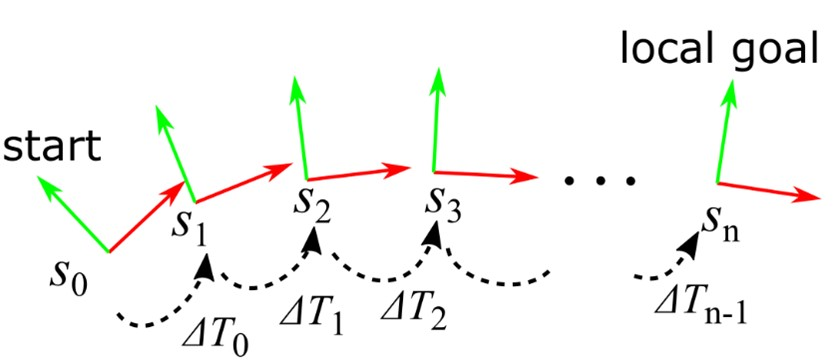
\includegraphics[width=.6\linewidth]{img/auto_28.jpg}
      \caption{最適化前}
      \label{auto:teb:before}
    \end{center}
  \end{figure}
  \begin{figure}[h]
    \begin{center}
      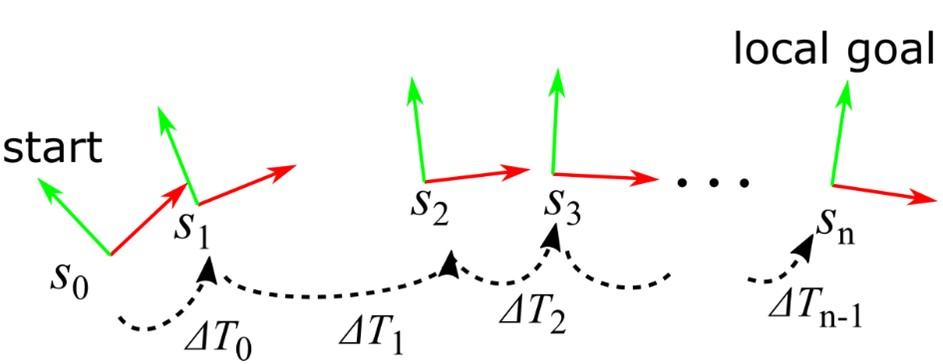
\includegraphics[width=.6\linewidth]{img/auto_29.jpg}
      \caption{最適化後}
      \label{auto:teb:after}
    \end{center}
  \end{figure}
\begin{figure}[h]
  \begin{center}
    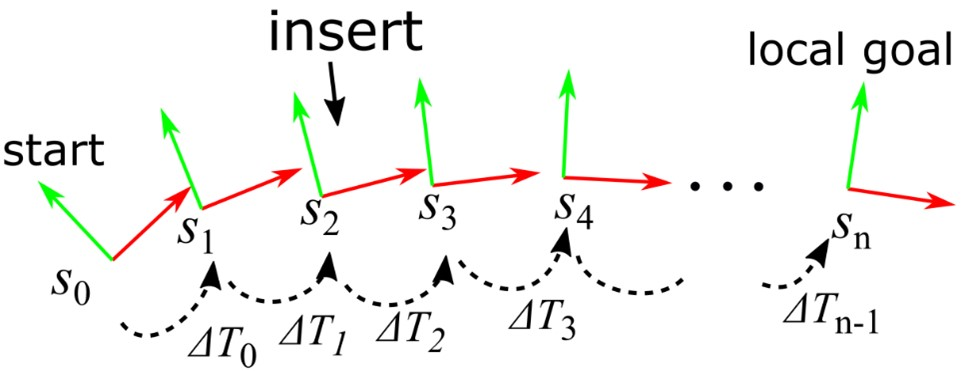
\includegraphics[width=.6\linewidth]{img/auto_30.jpg}
    \caption{auto resizing後}
    \label{auto:teb:resizing}
  \end{center}
\end{figure}
\item TEBの最適化処理の流れ\\
Navigation Stackから並進速度・角速度の計算要求があるたび、デフォルトでは、auto resizing(Insert/delete TEB states)、Hyper-graphの最適化(5回のLevenberg-Marquardtの反復)という流れを4回反復する。
\begin{figure}[h]
  \begin{center}
    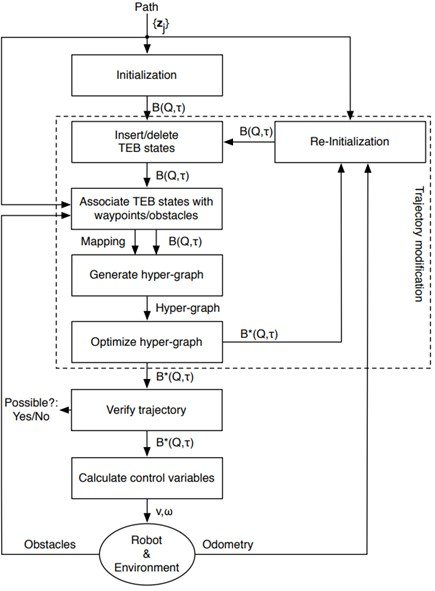
\includegraphics[width=.6\linewidth]{img/auto_31.jpg}
    \caption{TEBの最適化プロセス}
    \label{auto:teb:opt}
  \end{center}
\end{figure}
\item 初期軌道生成\\
TEBでは軌道を連続的に変形するため、障害物をまたぐような変形が行われない。そこで、複数の軌道を扱えるようにするために、HomotopyClassPlanner\cite{auto:teb3}が使われる。Homotopy Classには以下のような定義がある。
\begin{enumerate}
  \item 定義1:(Homotopy)同じ始点と終点を結ぶ二つの軌道は、一方が障害物と交差することなく他方に連続的に変形できる。
  \item 定義2:(Homotopy Class)互いにHomotopyである全ての軌道の集合
\end{enumerate}
複数の軌道を扱う際、同じHomotopy classに属する軌道は1つあれば充分であるため、Homotopy classの判定を行って、フィルタリングを行う。
\item 複数の軌道を扱う際、同じHomotopy classに属する軌道は1つあれば充分であるため、Homotopy classの判定を行って、フィルタリングを行う。
\item H-signatureによるHomotopy classの判定\\
Homotopy classに属する軌跡$\tau$ に対して不変な量を以下のように定義する。
\begin{align*}
  \mathcal{H}(\tau)=\int_{\tau}\mathcal{F}(z) \,dz\\
  \mathcal{F}(z)=\frac{f_0(z)}{(z-\xi_1) (z-\xi_2) \ldots (z-\xi_R)}
\end{align*}
ここで、$\xi_k$は、障害物の代表点である。この不変量H-signatureを数値的に(離散的な軌跡に対して)計算すると、2つの軌跡の間のH-signatureを比較することによって、
同じHomotopy classに属するか否かの判定を行うことができる。(実部と虚部でそれぞれ差の絶対値を計算して、閾値より小さければ同じHomotopy classに属す)
以下の図\ref{auto:teb:seisei}に初期軌道生成から最適化までの処理を示す。

\begin{figure}[h]
  \begin{center}
    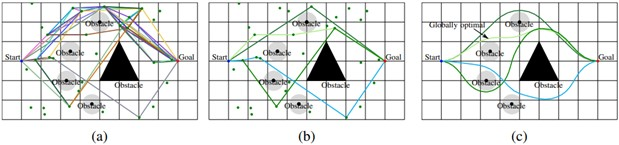
\includegraphics[width=\linewidth]{img/auto_32.jpg}
    \caption{初期軌道生成から最適化までの処理}
    \label{auto:teb:seisei}
  \end{center}
\end{figure}
\begin{enumerate}
  \item 頂点のサンプリングを行う。
  \item スタートの頂点から、ゴールに近づき、かつ線分が障害物と交差しないようにエッジを作成する。さらに、スタートの頂点とエッジで接続された頂点から、
  ゴールに近づき、かつ線分が障害物と交差しないようにエッジを作成するという処理を繰り返す。(図(a))
  \item スタートからゴールまでの各パスに対して、H-signatureを計算して、新しいHomotopy classであれば、軌跡とH-signatureを保存する。
  \item 各軌跡をTEBで最適化する。
\end{enumerate}
\end{enumerate}

\subsubsection{アッカーマンステアリングジオメトリ}
Navigaton Stackの軌道計画に与える制約条件を求めるために、
本研究で用いるシステムの旋回角度を求める。
図\ref{auto:tokusei}のようにすることで、サーボモータの制御パルス値と旋回角度(切れ角)の対応値を取得する。
本研究の自動運転システムに用いたRCカーのステアリング機構は、図\ref{auto:para}パラレルステアリングジオメトリである。
軌道計画に運動学が簡単なアッカーマンステアリングジオメトリが採用されているため、
ステアリング機構を図\ref{auto:ackermann}に示すアッカーマンステアリングジオメトリへの改造を行った。
図\ref{auto:ackerk}、式\eqref{auto:eq:ackermann}にアッカーマンステアリングジオメトリと、その運動学を示す。

\begin{figure}[h]
  \begin{center}
  \subfigure[改良前のRCカー(パラレルステアリングジオメトリ)]{
  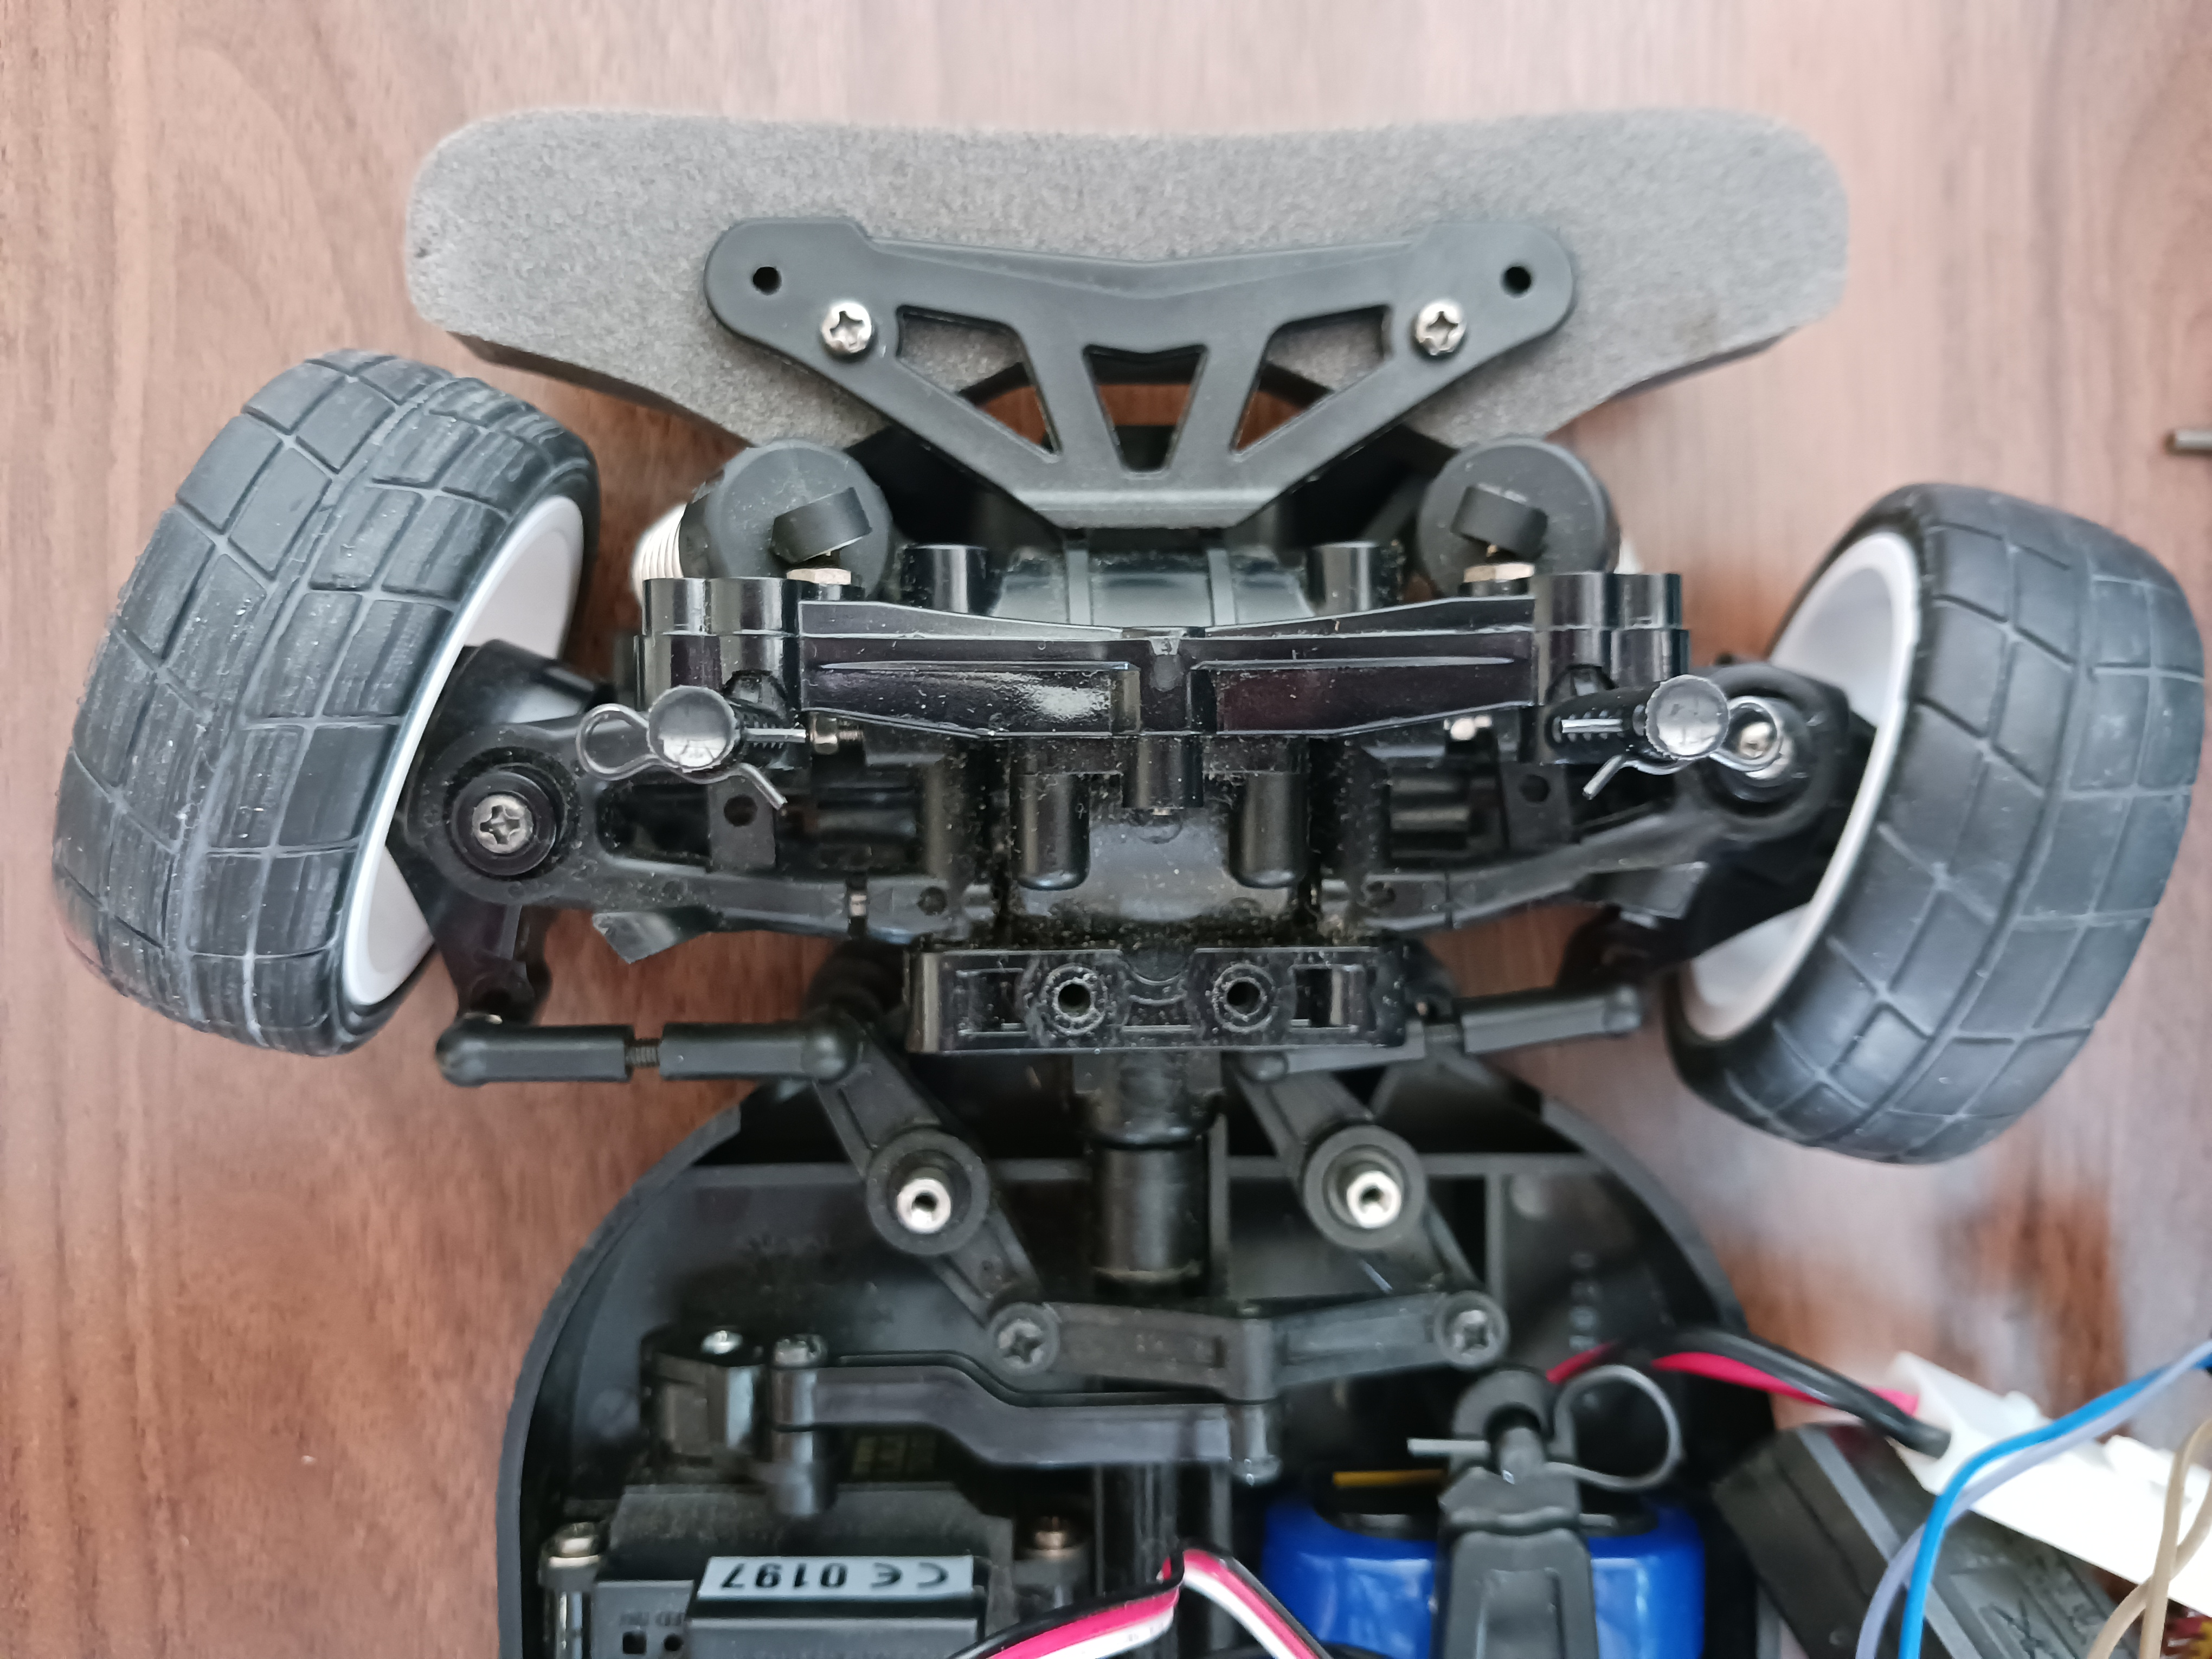
\includegraphics[width=.45\columnwidth]{img/auto_33.jpg}
  \label{auto:para}
  }
  \subfigure[DS上コースの寸法:全長]{
  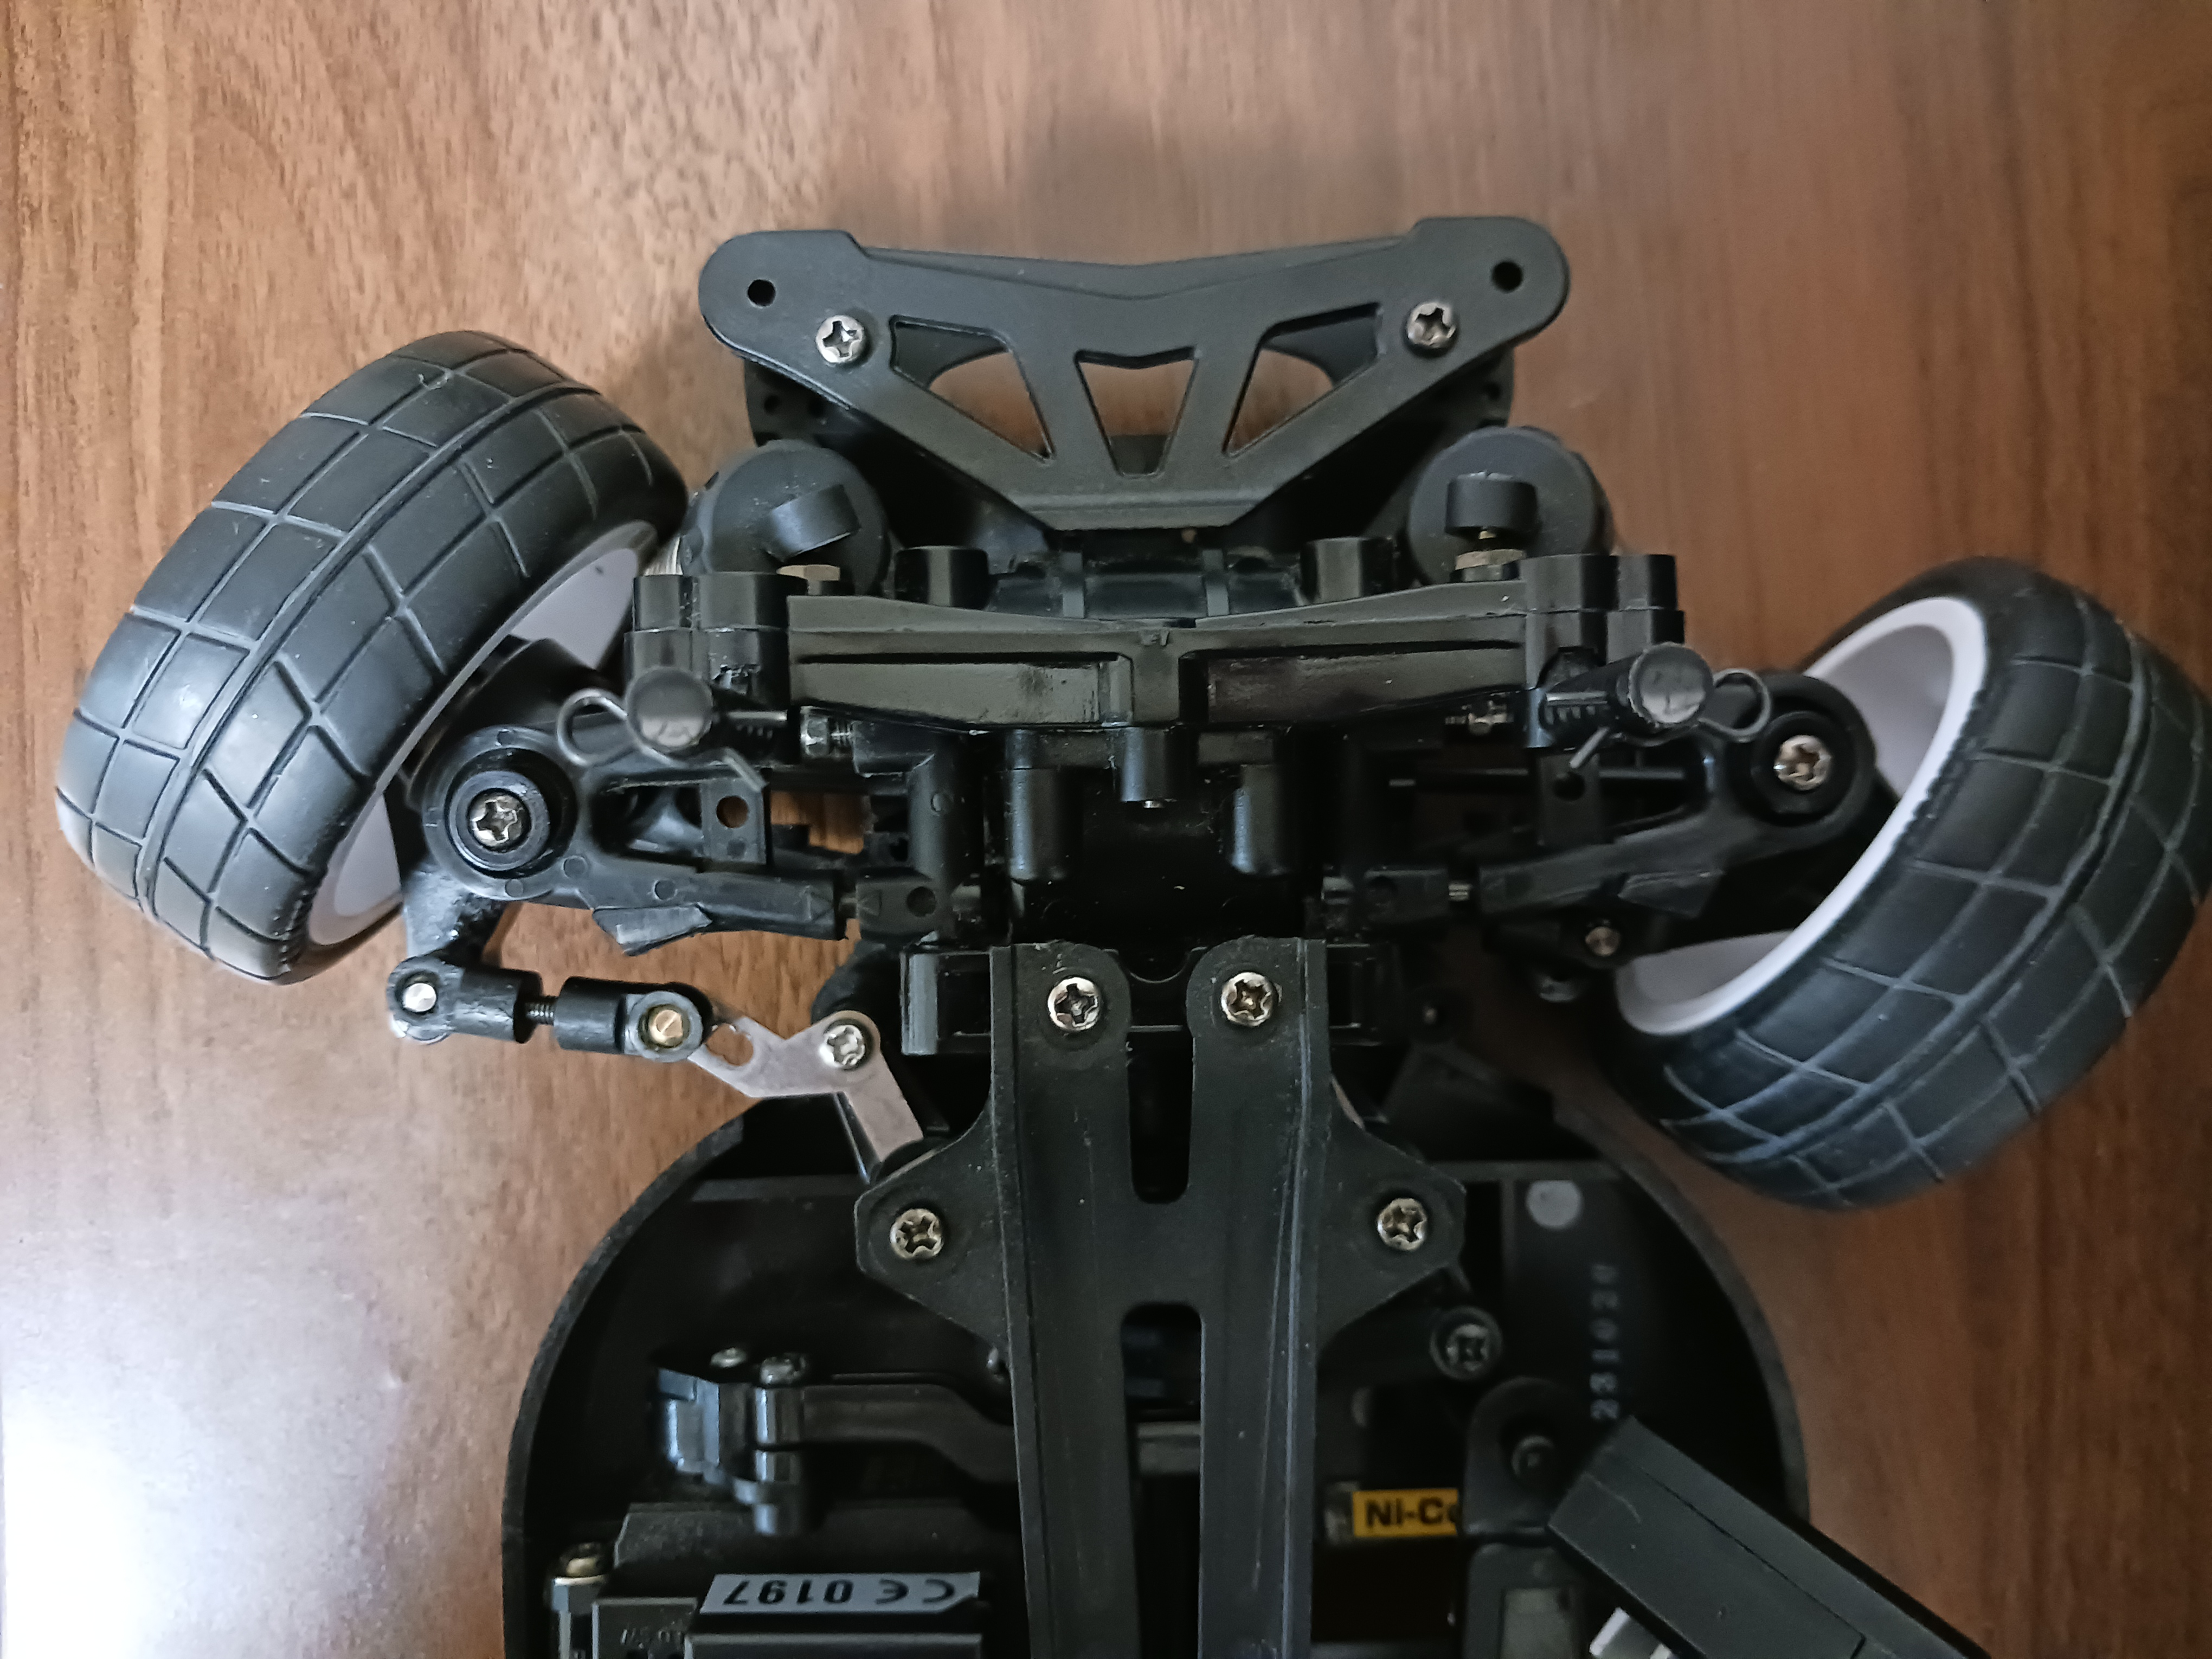
\includegraphics[width=.45\columnwidth]{img/auto_34.jpg}
  \label{auto:ackermann}
  }
  \caption{本研究で使用したRCカーの改造}
  \label{auto:rc}
  \end{center}
\end{figure}

\begin{figure}[h]
  \begin{center}
    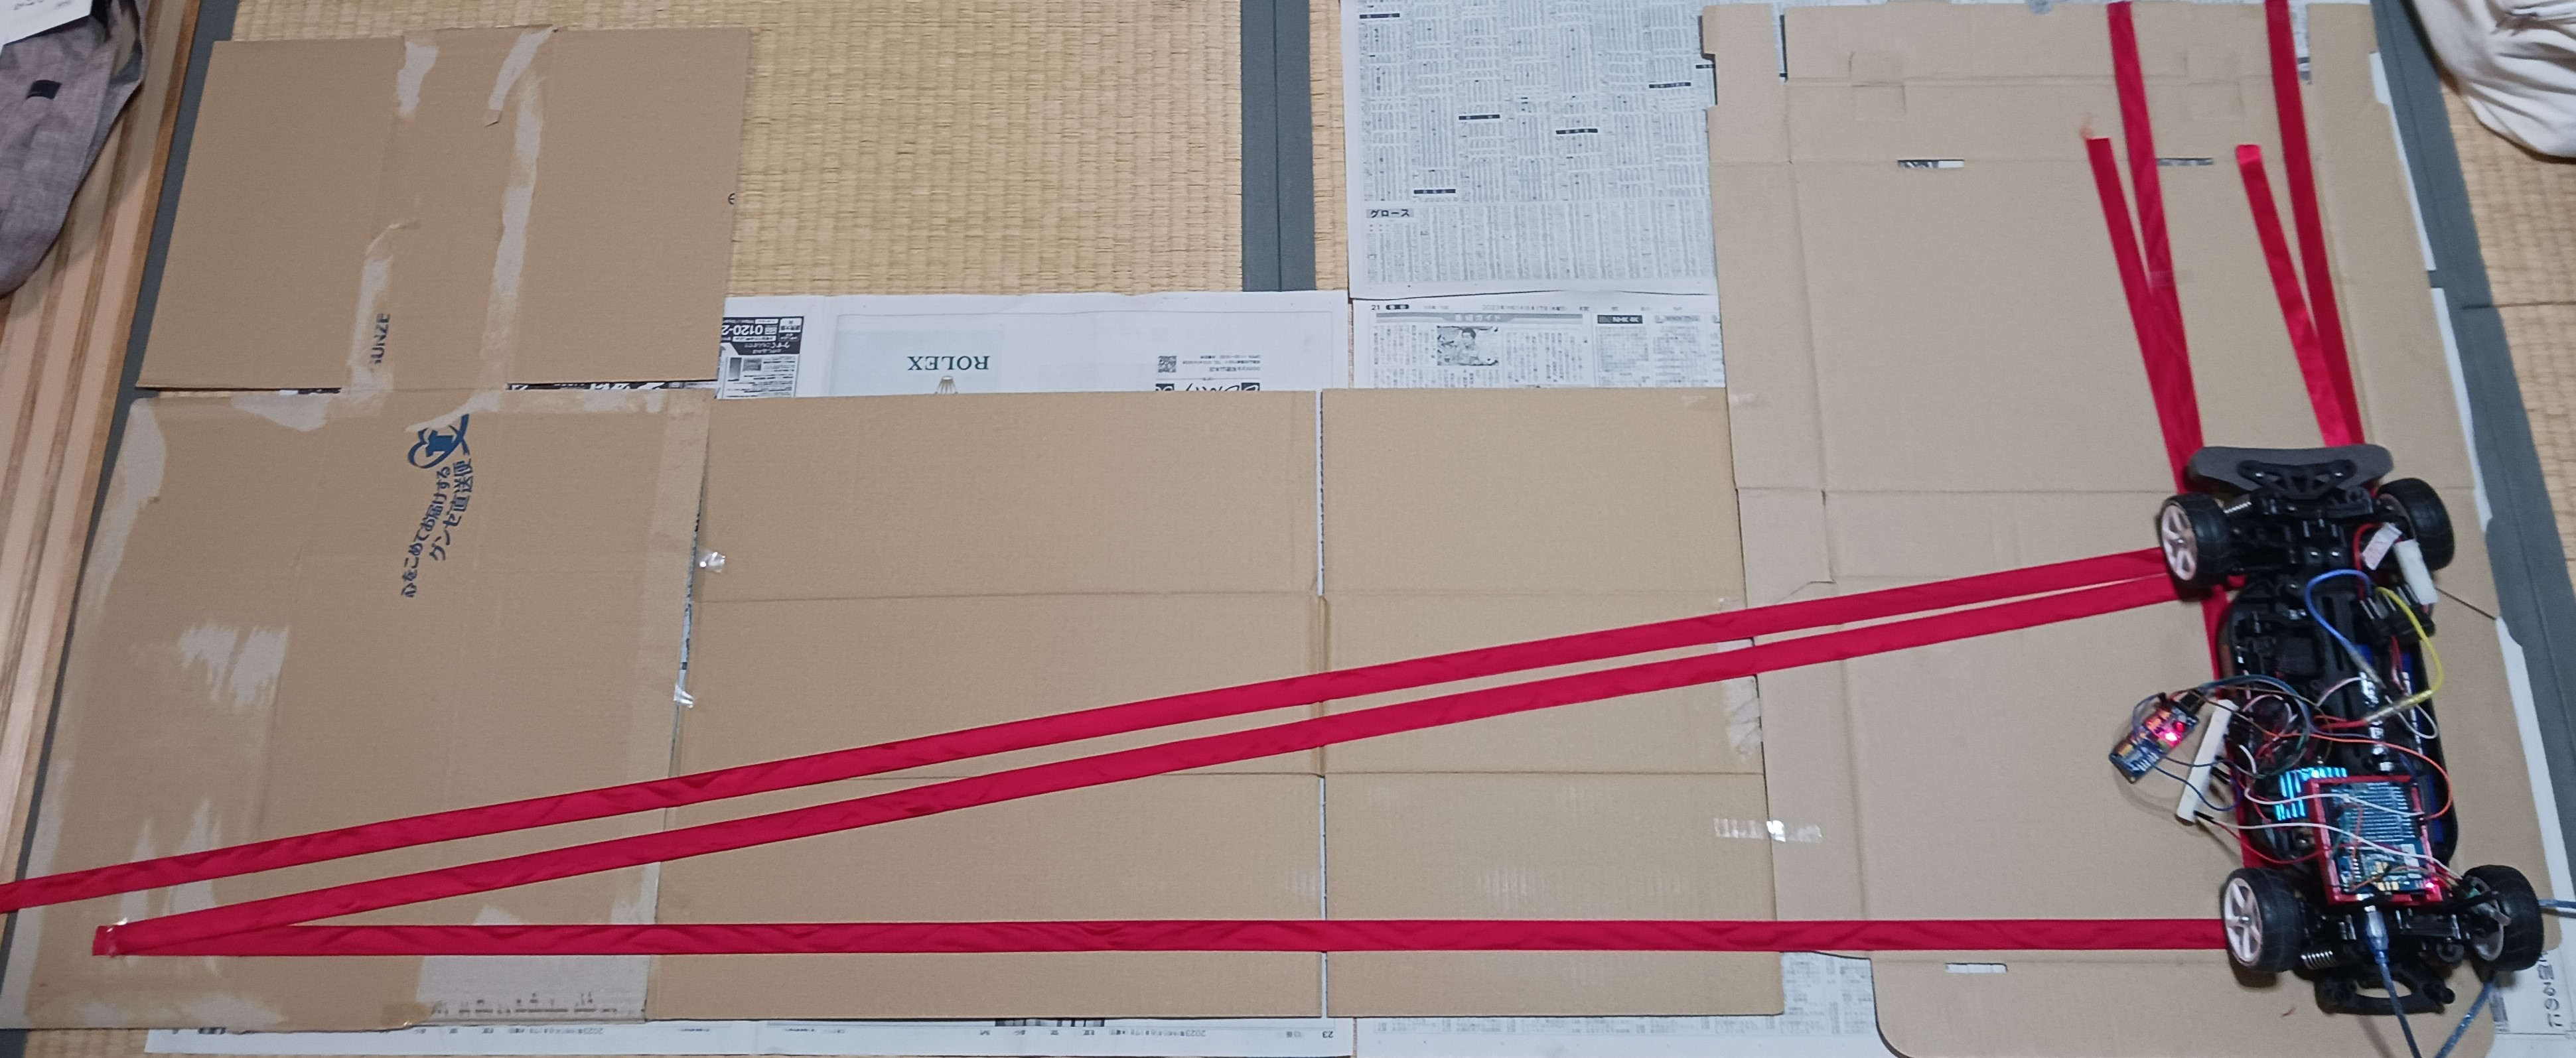
\includegraphics[width=.9\linewidth]{img/auto_35.jpg}
    \caption{切れ角とサーボモータの制御パルス値の特性取得}
    \label{auto:tokusei}
  \end{center}  
\end{figure}

\begin{align}
  \phi = \arctan\frac{wheelbase}{r} = \arctan\frac{\omega \cdot wheelbase}{v} \label{auto:eq:ackermann}
\end{align}

\begin{figure}[h]
  \begin{center}
    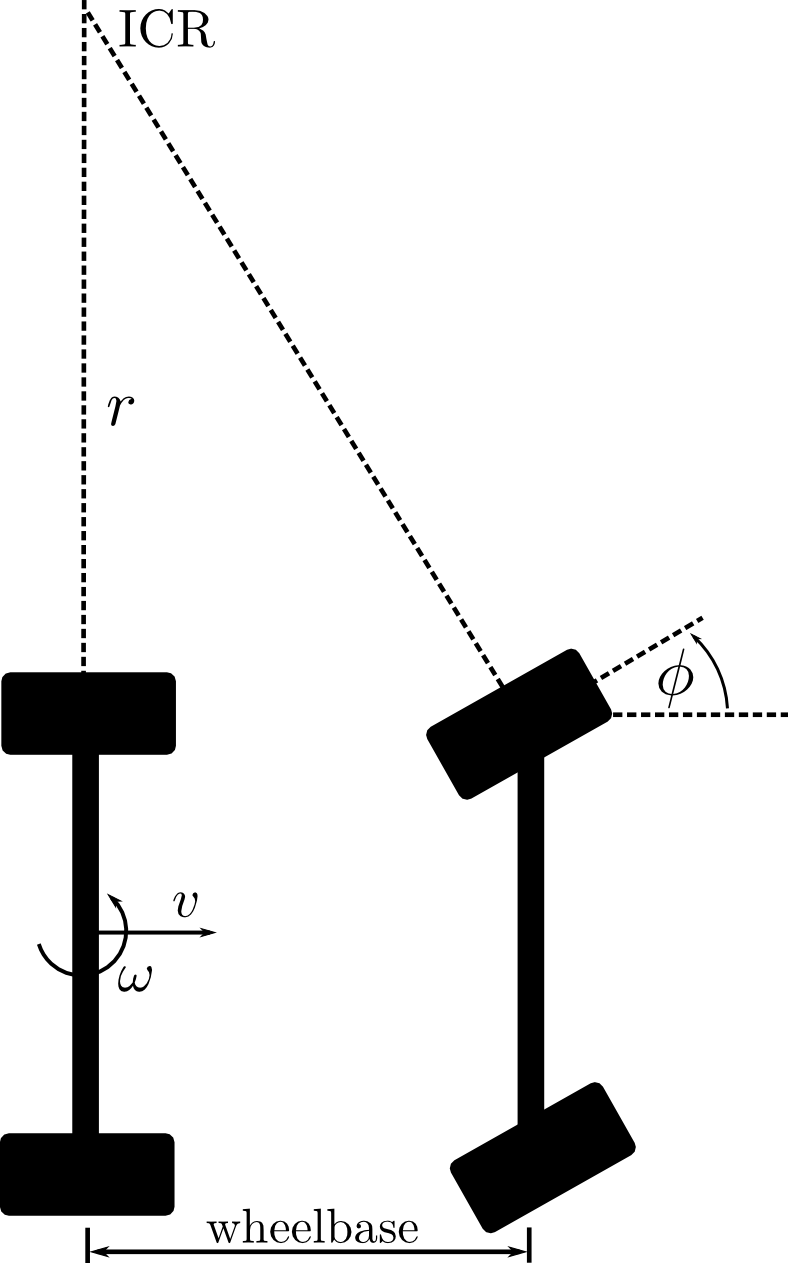
\includegraphics[width=.3\linewidth]{img/auto_36.png}
    \caption{アッカーマンステアリングジオメトリの運動学\cite{auto:teb:ackermann}}
    \label{auto:ackerk}
  \end{center}  
\end{figure}

アッカーマンステアリングでは、式\eqref{auto:eq:ackermann}に基づいて、角速度の値からステアリング角度を計算する。
ステアリング角度をサーボモータの制御パルス値へと変換した際に取得した特性を図\ref{auto:tokusei2}に示す。
また、前進・後退の速度値は適当な定数を掛け合わせて、DCモータの制御パルス値に変換しているため、
速度の精度は厳密ではない。前進・後退時の速度は前進を0.06 \si{[m/s]}、
後退を0.05 \si{[m/s]}として、DCモータの制御パルスとの特性を一次関数的に近似した。
\begin{figure}[h]
  \begin{center}
    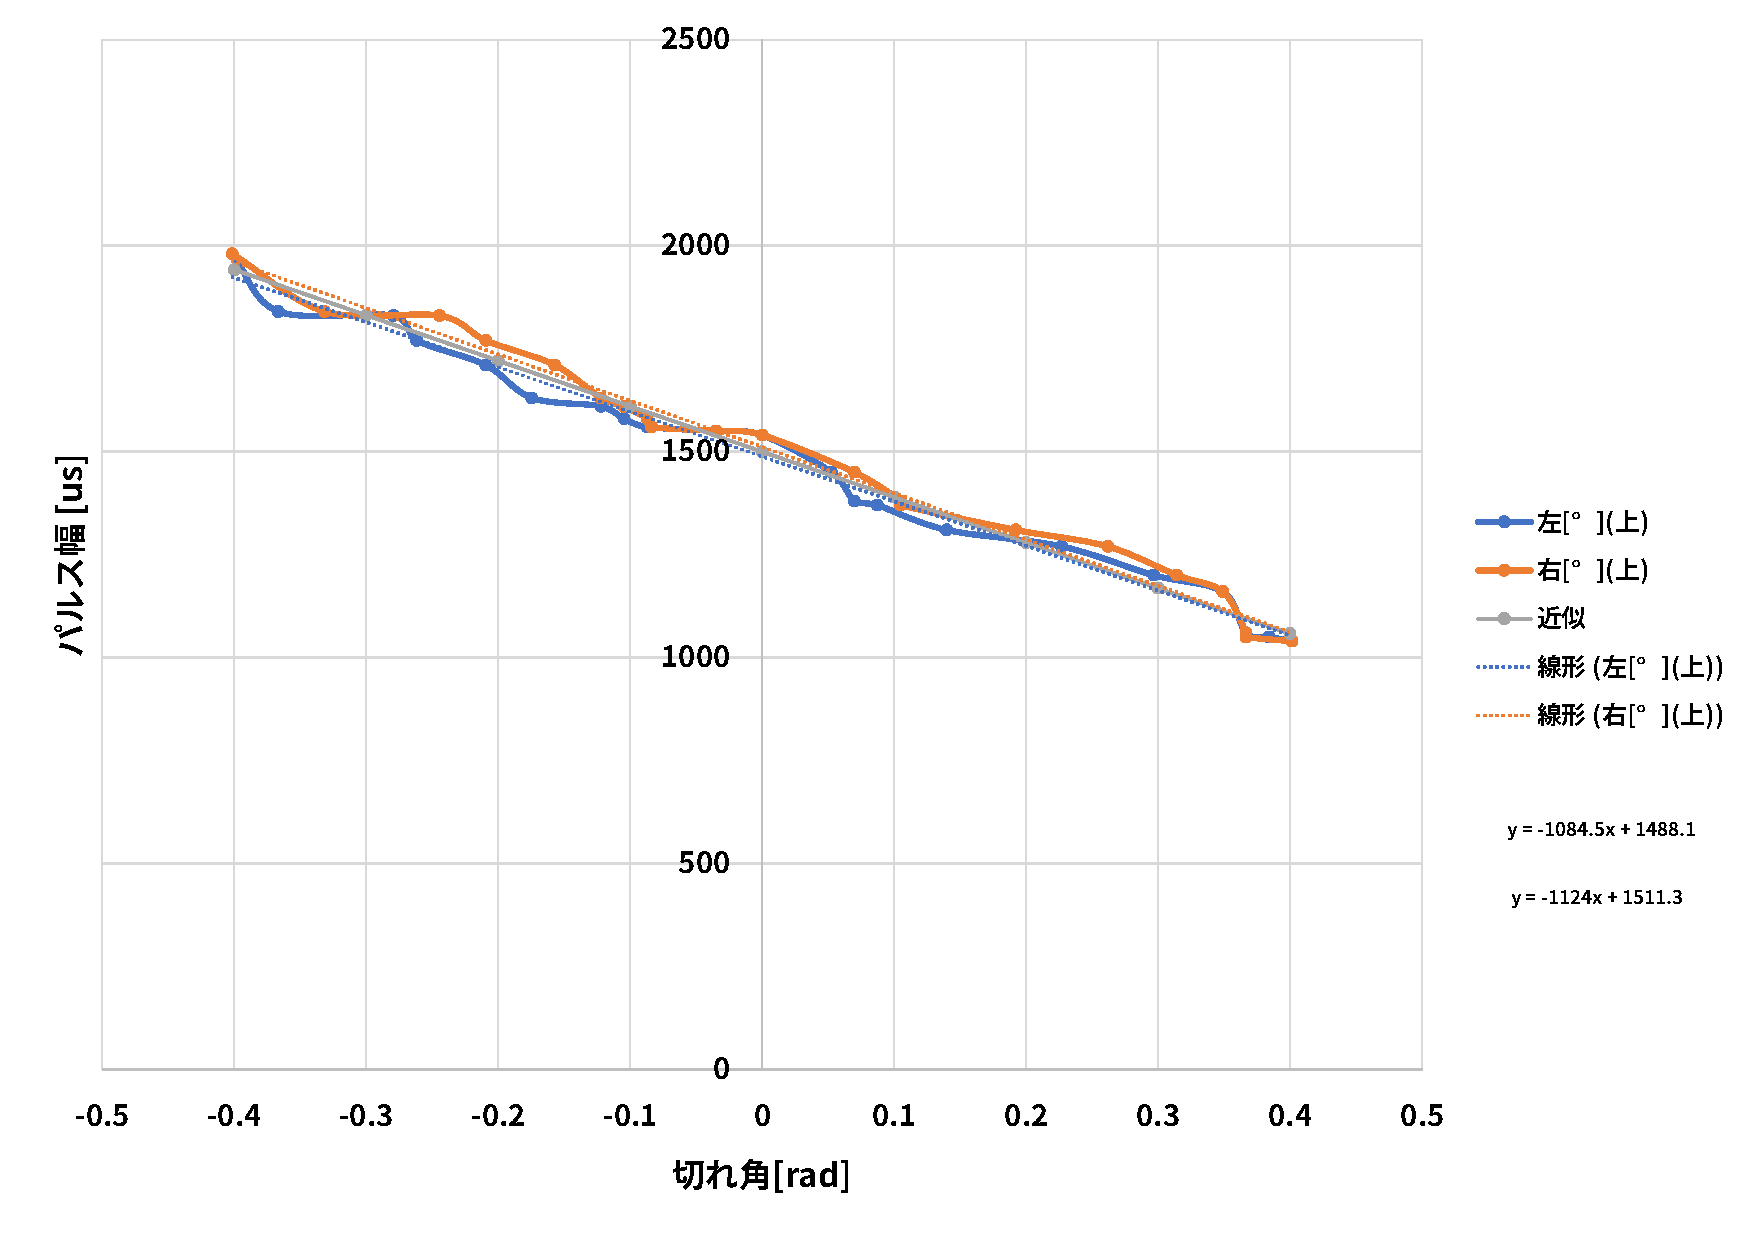
\includegraphics[width=.8\linewidth]{img/auto_37.pdf}
    \caption{ステアリング角度とモータの制御パルス値へと変換した特性}
    \label{auto:tokusei2}
  \end{center}
\end{figure}


\subsubsection{コストマップ}
\verb|costmap_2d|パッケージ\cite{auto:costmap2d}は、ロボットが占有格子の形式でナビゲーションを行う場所に関する情報を提供する。
コストマップは、制約マップのセンサデータと情報を使用して、\verb|costmap_2d::Costmap2D|ROSオブジェクトを介して、
空間の障害物に関する情報を保存および更新する。つまり、障害物の判定は"列"単位でのみ行うことができる。
たとえば、XY平面で同じ位置にあるがZ位置が異なるテーブルと靴の場合\verb|costmap_2d::Costmap2D|ROSオブジェクトのコストマップの対応するセルのコスト値は同じになる。
これは、平面空間での経路探索がしやすいように設計されている。

\begin{figure}[h]
  \begin{center}
    \subfigure[costmapの概要]{
      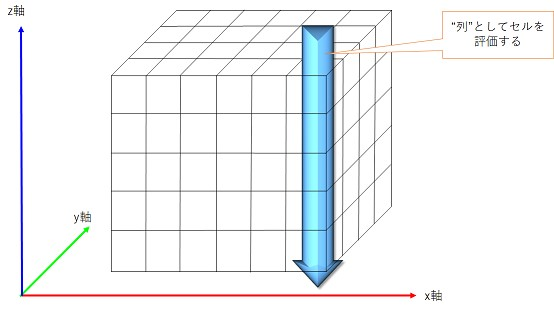
\includegraphics[width=.6\linewidth]{img/auto_38.jpg}
      \label{auto:costmap_search}
      }
    \subfigure[2次元のcostmap]{
      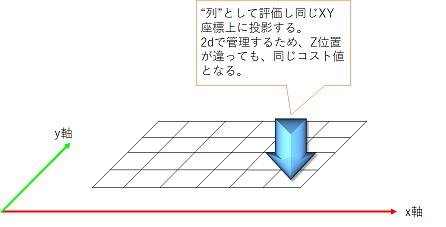
\includegraphics[width=.6\linewidth]{img/auto_39.jpg}
      \label{auto:costmap_2d}
      }
  \caption{コストマップ}
  \label{auto:costmap_gaiyou}
  \end{center}
\end{figure}

\begin{enumerate}
  \item マークとクリア\\
  コストマップは、ROSを介してセンサートピックを自動的にサブスクライブし、それに応じて更新させる。各センサは、
  マーク(障害物情報をコストマップに挿入)、クリア(障害物情報をコストマップから削除)、またはその両方に使用される。
  マーク操作は、セルのコストを変更するための配列への単なるインデックスである。しかしながらクリア操作は、レポート
  される各観測について、センサの原点から外側に向かってグリッドを通過するレイトレーシングで構成される。3次元構造を使用して
  障害物情報を保存する場合、各列からの障害物情報は、コストマップに配置されるときに2次元に投影される。
  \begin{figure}[h]
    \begin{center}
      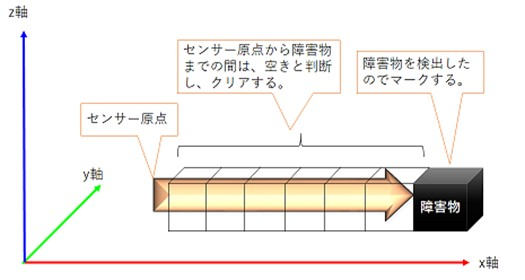
\includegraphics[width=.6\linewidth]{img/auto_40.jpg}
      \caption{マークのクリア}
      \label{auto:mark_clear}
    \end{center}
  \end{figure}
  \item 占有・空き・未知スペース\\
  コストマップの各セルには255の異なるコスト値のいずれかを持つことができるが、使用する基本構造は3つの状態のみを表すことができる。
  具体的に、この構造の各セルは、空き、占有、未知スペースのいずれかである。
  各ステータスには、コストマップへの投影時に割り当てられる、特別なコスト値がある。 
  一定数の占有セルがある列には\verb|costmap_2d::LETHAL_OBSTACLE|コストが割り当てられ、一定数の未知のセル(\verb|unknown_threshold|パラメータを参照)がある列には
  \verb|costmap_2d::NO_INFORMATION|コストが割り当てられ、その他の列には\verb|costmap_2d::FREE_SPACE|コストが割り当てられる。
  \item マップの更新\\
  コストマップは、\verb|update_frequency|パラメータで指定された周期でマップ更新サイクルを実行する。周期ごとに、センサデータが入力され、マークとクリアの操作がコストマップの基本的な占有構造で実行される。
  この構造は上記のように適切なコスト値が割り当てられるコストマップに投影される。その後、障害物のインフレーションは\verb|costmap_2d::LETHAL_OBSTACLE|コストを持ったそれぞれのセルで実行される。
  これは、占有されている各セルからユーザ定義のインフレーション半径までコスト値を外側に伝播することで構成される。このインフレーション処理の詳細を以下に示す。
  \item tf\\
  センサソースからコストマップデータを挿入するために、\verb|costmap_2D::Costmap2D| ROSオブジェクトは、tfを広範囲に使用する。
  具体的に、\verb|global_frame|パラメータ、センサーソースが接続され、最新である想定で使用している。\verb|transform_tolerance|
  パラメータは、これらの変換間で許容されるレイテンシーの最大量を設定する。tfツリーがこの予想されるレートで更新されない場合、Navigation Stackはロボットを停止する。
  \item インフレーション\\
  インフレーションは、距離とともに減少する占有セルからコスト値を伝播するプロセスである。この目的のために、ロボットに関連するコストマップ値に5つの特定のシンボルを定義する。
  \begin{enumerate}
    \item 「致命的」コスト(\verb|cost_lethal|)とは、セルに障害物があることを意味する。そのため、ロボットの中心がそのセルにある場合、ロボットは間違いなく衝突している。
    \item 「内接」コスト(\verb|cost_inscribed|)とは、セルと実際の障害物の距離が、ロボットの内接半径より小さいことを意味する。従って、ロボットの中心が内接コスト以上のセル内にある場合、
    ロボットは確実に障害物と衝突する。
    \item 「おそらく外接」コスト(\verb|cost_possibly_circumscribed|)は「内接」に似ているが、ロボットの外接半径を限界距離として扱う。したがって、ロボットの中心がこの値以上のセル内にある場合、障害物と衝突するかどうかはロボットの向きによって決まる。
    「おそらく」という言葉を用いるのは、実際には、障害物ではなく、ユーザ設定値によりこのコスト値となっているセルの可能性があるためである。例えば、ユーザが、ロボットが建物の特定の領域を回避するように表現したい場合、障害物に関係なく、その領域のコストマップに独自のコスト値を挿入する場合がある。
    \item 「空き」コスト(freespace cost)はゼロであると想定される。これは、ロボットがそこに行くのを妨げるものが無いことを意味する。
    \item 「未知」コストは、特定のセルに関連する技術がないことを意味する。コストマップのユーザは適切に解釈することができる。
    \item 他の全てのコストには「致命的」セルからの距離と、ユーザが提供する減衰関数に応じて、「空き」と「おそらく外接」の間の値が割り当てられる。
    \\図\ref{auto:costmap_2D}にコストマップの設定変数を示す。
    \begin{figure}[h]
      \begin{center}
        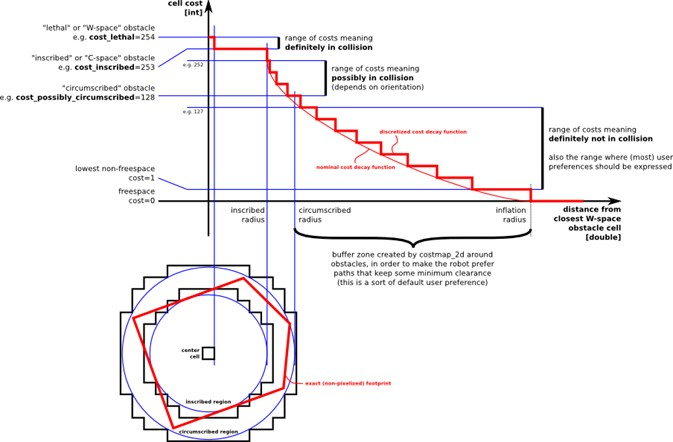
\includegraphics[width=.8\linewidth]{img/auto_41.jpg}
        \caption{コストマップの設定変数}
        \label{auto:costmap_2D}
      \end{center}
    \end{figure}
  \end{enumerate}
\end{enumerate}

\subsubsection{地図の保存と再読み込み}
地図の保存にはROSの\verb|map_server|、\verb|map_saver|を使用する。これらにより、LiDARによって取得した地図をコマンド入力により、
pgm形式で保存する。

\subsection{Waypoint Navigationの実装}
\subsubsection{waypointの設定・保存・可視化}
図\ref{auto:csv_waypoint}に、waypointの保存と可視化を示す。
RViz上でwaypointを設定し、csv形式で保存する。Navigationを行う際に、RViz上に地図の読み込みとwaypointの
csvデータを読み込んでマーカで表示する。これらの機能をpythonにより実装する。

\begin{figure}[h]
  \begin{center}
    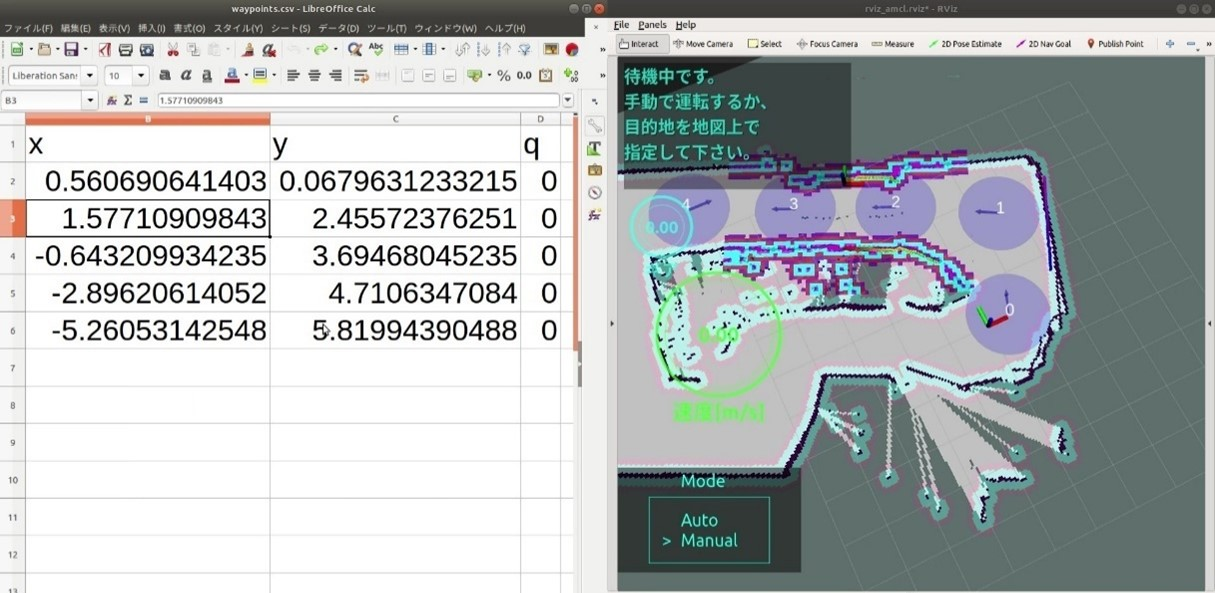
\includegraphics[width=.8\linewidth]{img/auto_42.jpg}
    \caption{waypointの保存と可視化}
    \label{auto:csv_waypoint}
  \end{center}
\end{figure}

\subsubsection{自動運転機能}
自動運転切り替え機能のノードを図\ref{auto:change}、図\ref{auto:change2}に示す。
保存した地図とwaypointのデータを読み込む。
初期位置からWaypointまでのナビゲーションを実行する。
Waypoint Navigationをする上で、次のwaypointへ到着する閾値を設定し、waypointから半径1m以内に到着したら、次のwaypointへのNavigationを開始する。
最後のwaypointを読み込んだならば、Navigationを終了する。これらを\verb|C++|言語により実装する。

\begin{figure}[h]
  \begin{center}
    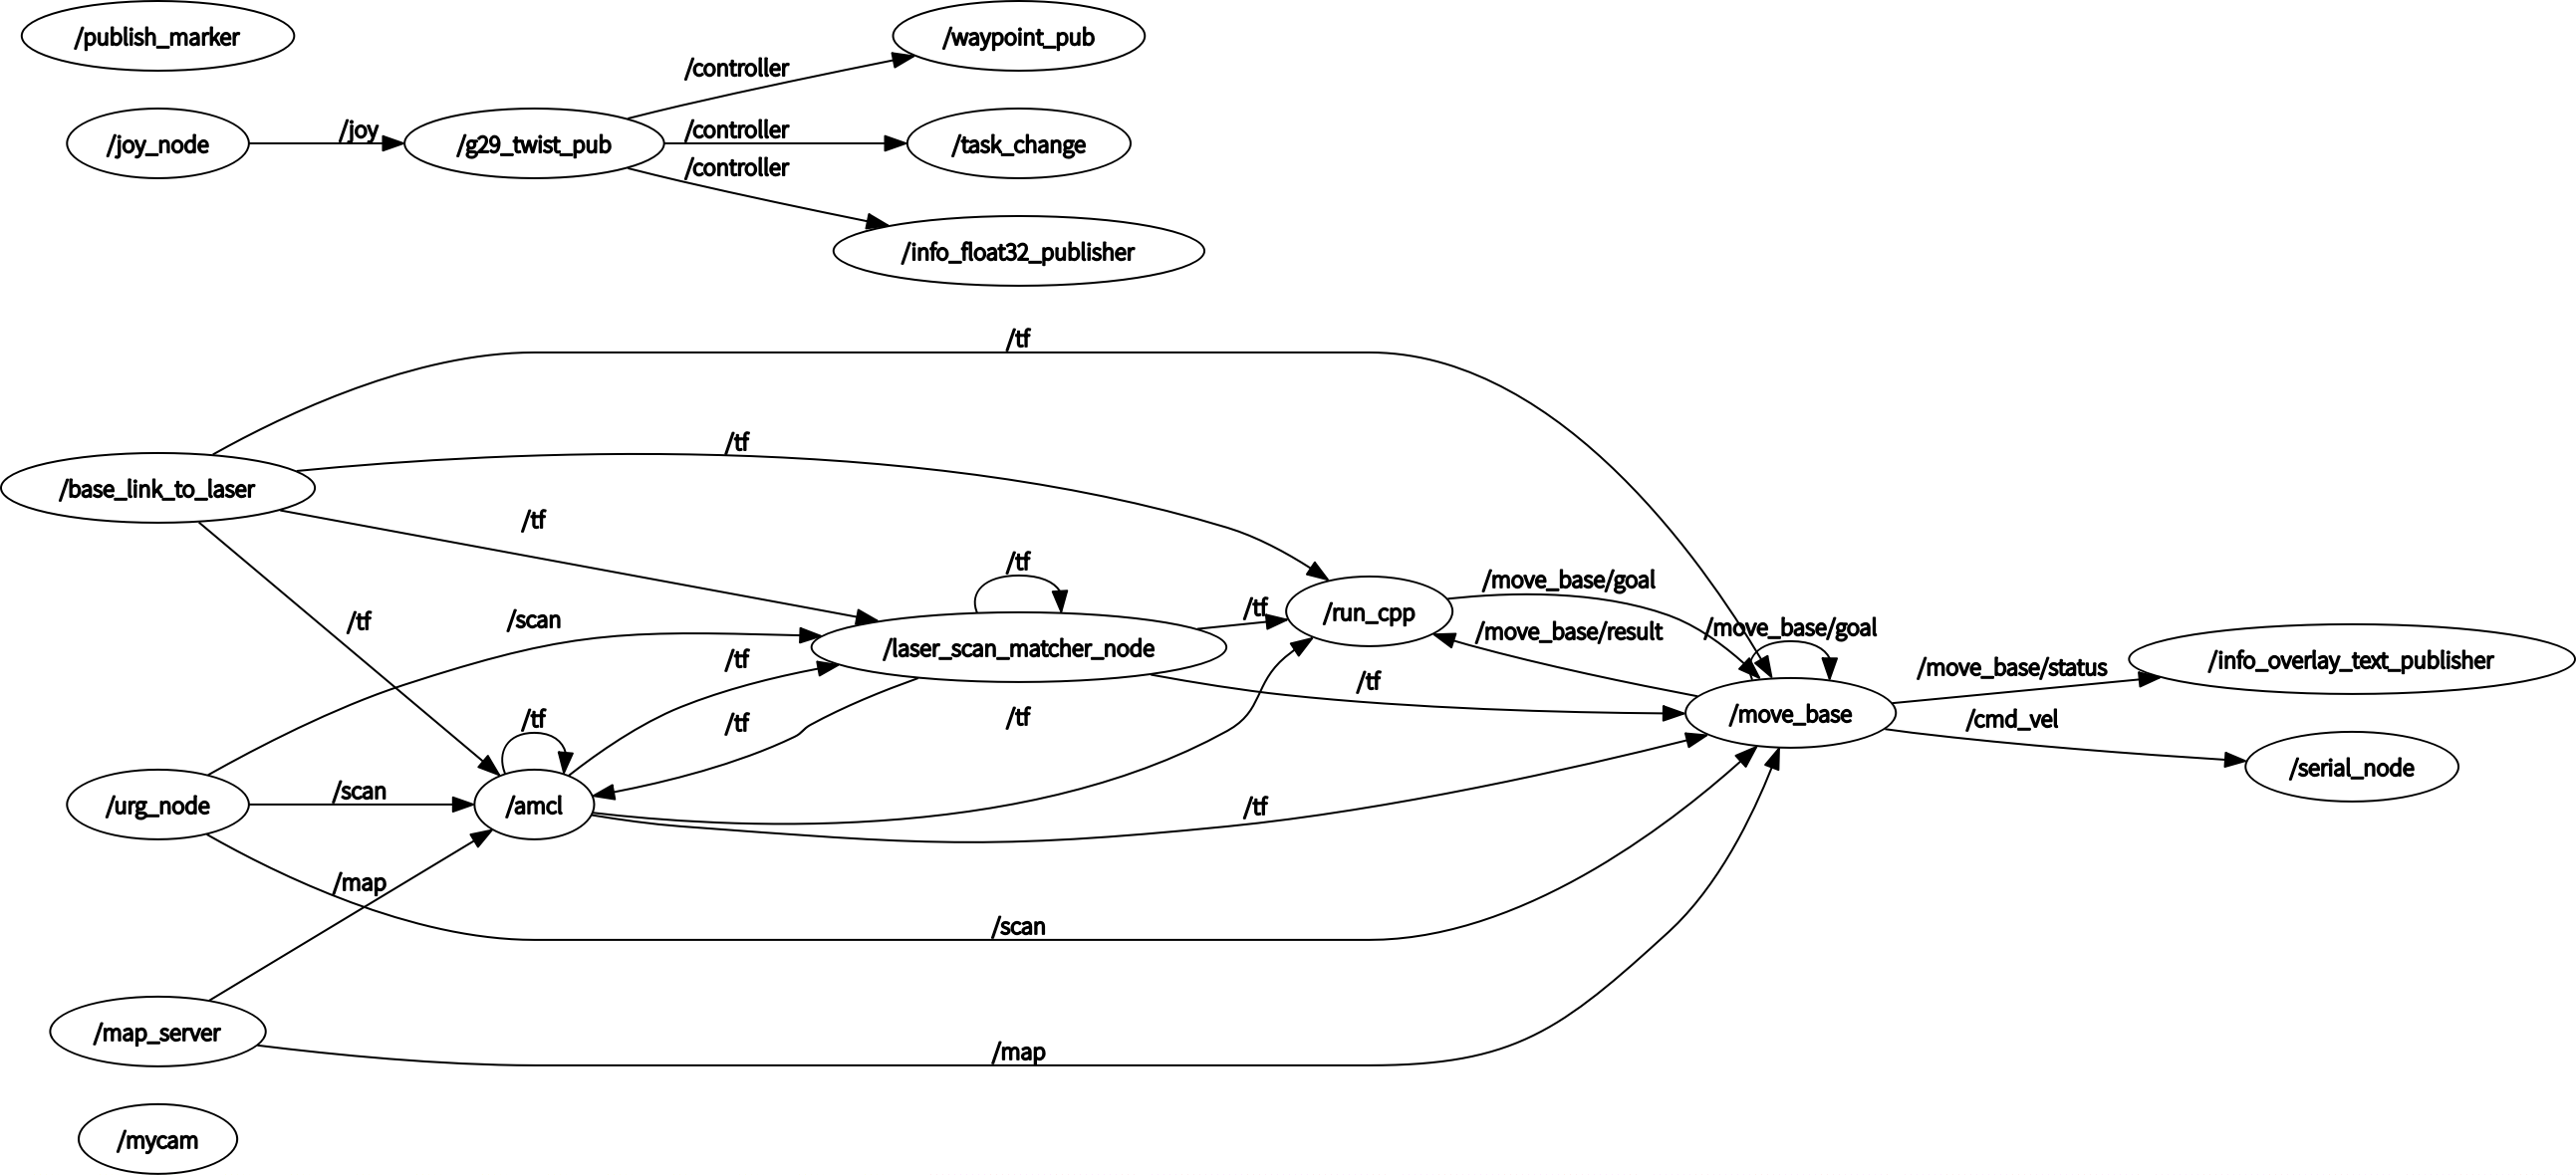
\includegraphics[width=\linewidth]{img/auto_43.png}
    \caption{自動運転切り替え機能のノード(トピック)}
    \label{auto:change}
  \end{center}
\end{figure}

\begin{figure}[h]
  \begin{center}
    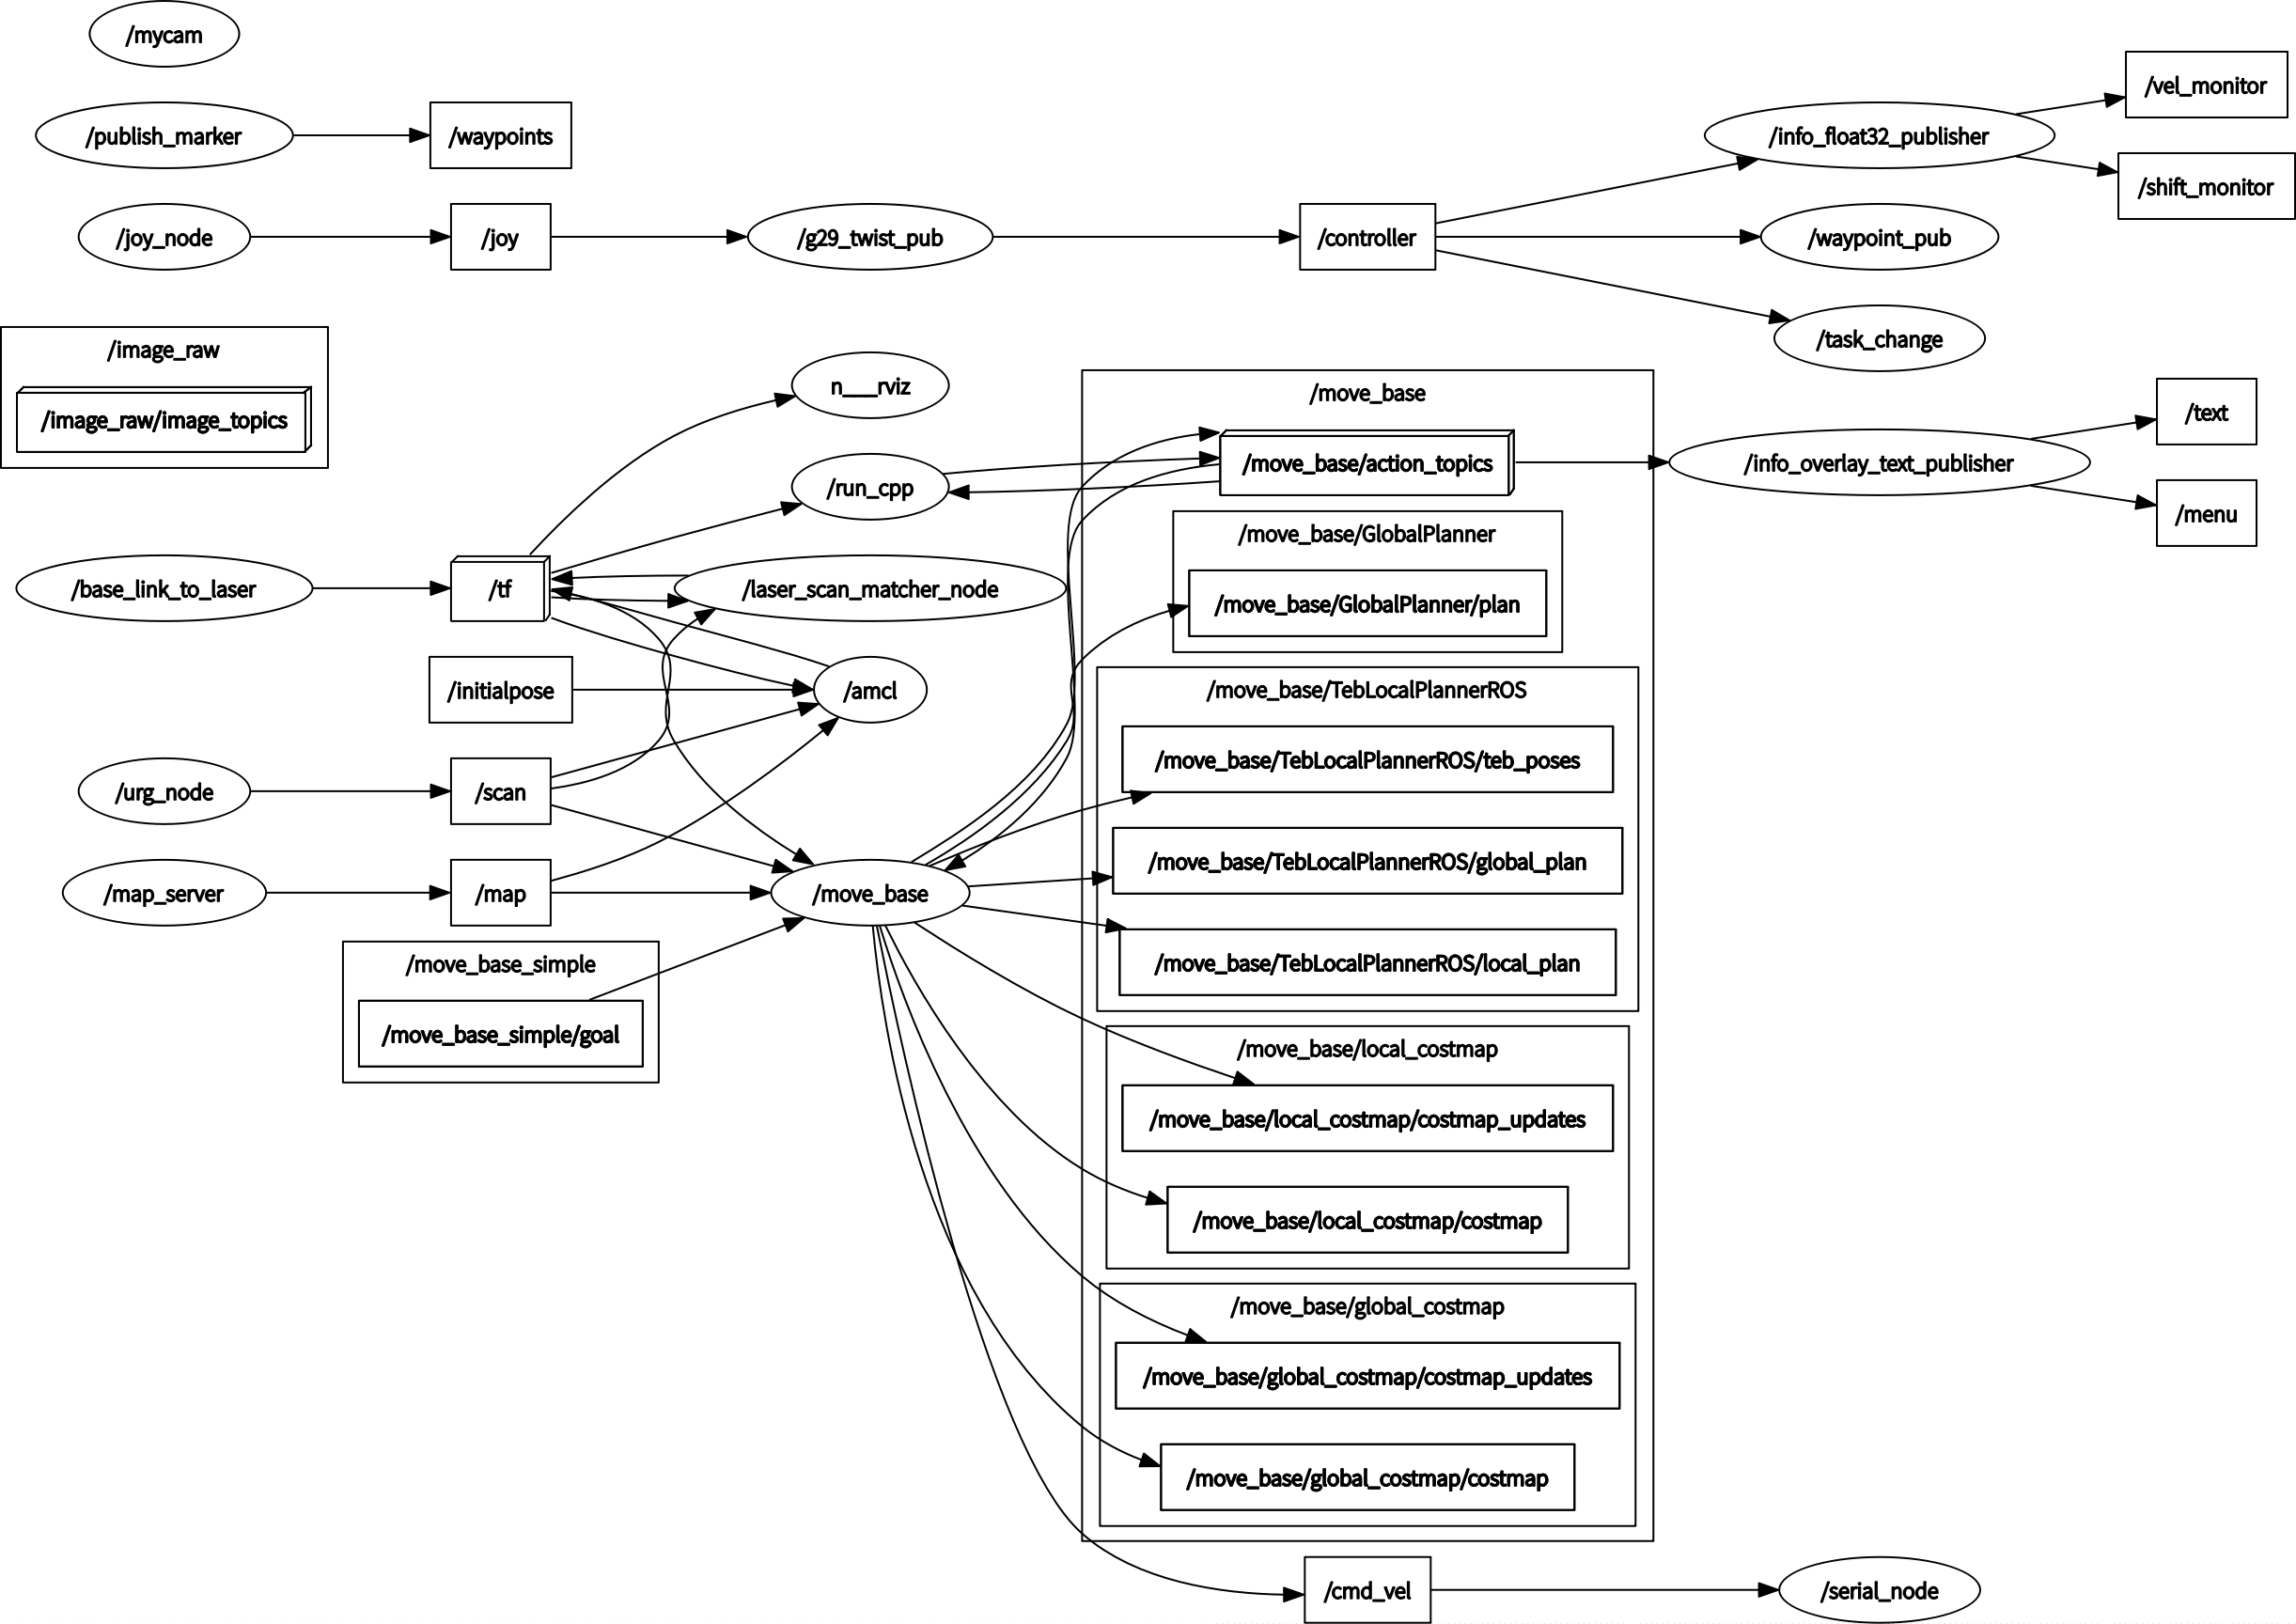
\includegraphics[width=\linewidth]{img/auto_44.png}
    \caption{自動運転機能の全体ノード}
    \label{auto:change2}
  \end{center}
\end{figure}

\subsection{自動運転と手動運転の引継ぎ機能の実装}
手動運転中、自動運転に切り替える機能において、手動操作と自動運転でトピックを共通にし、
コントローラのボタンを入力することで、手動運転のトピックを発行するノードをシャットダウンし、
自動運転のWaypoint Navigationを起動するようにする。また、自動運転から手動運転に切り替える際は、
Waypoint Navigationをシャットダウンし、手動運転のノードを起動する。これらをPythonにより実装する。
以上の機能を図\ref{auto:change_node}、\ref{auto:change_node2}に示す。

\begin{figure}[h]
  \begin{center}
    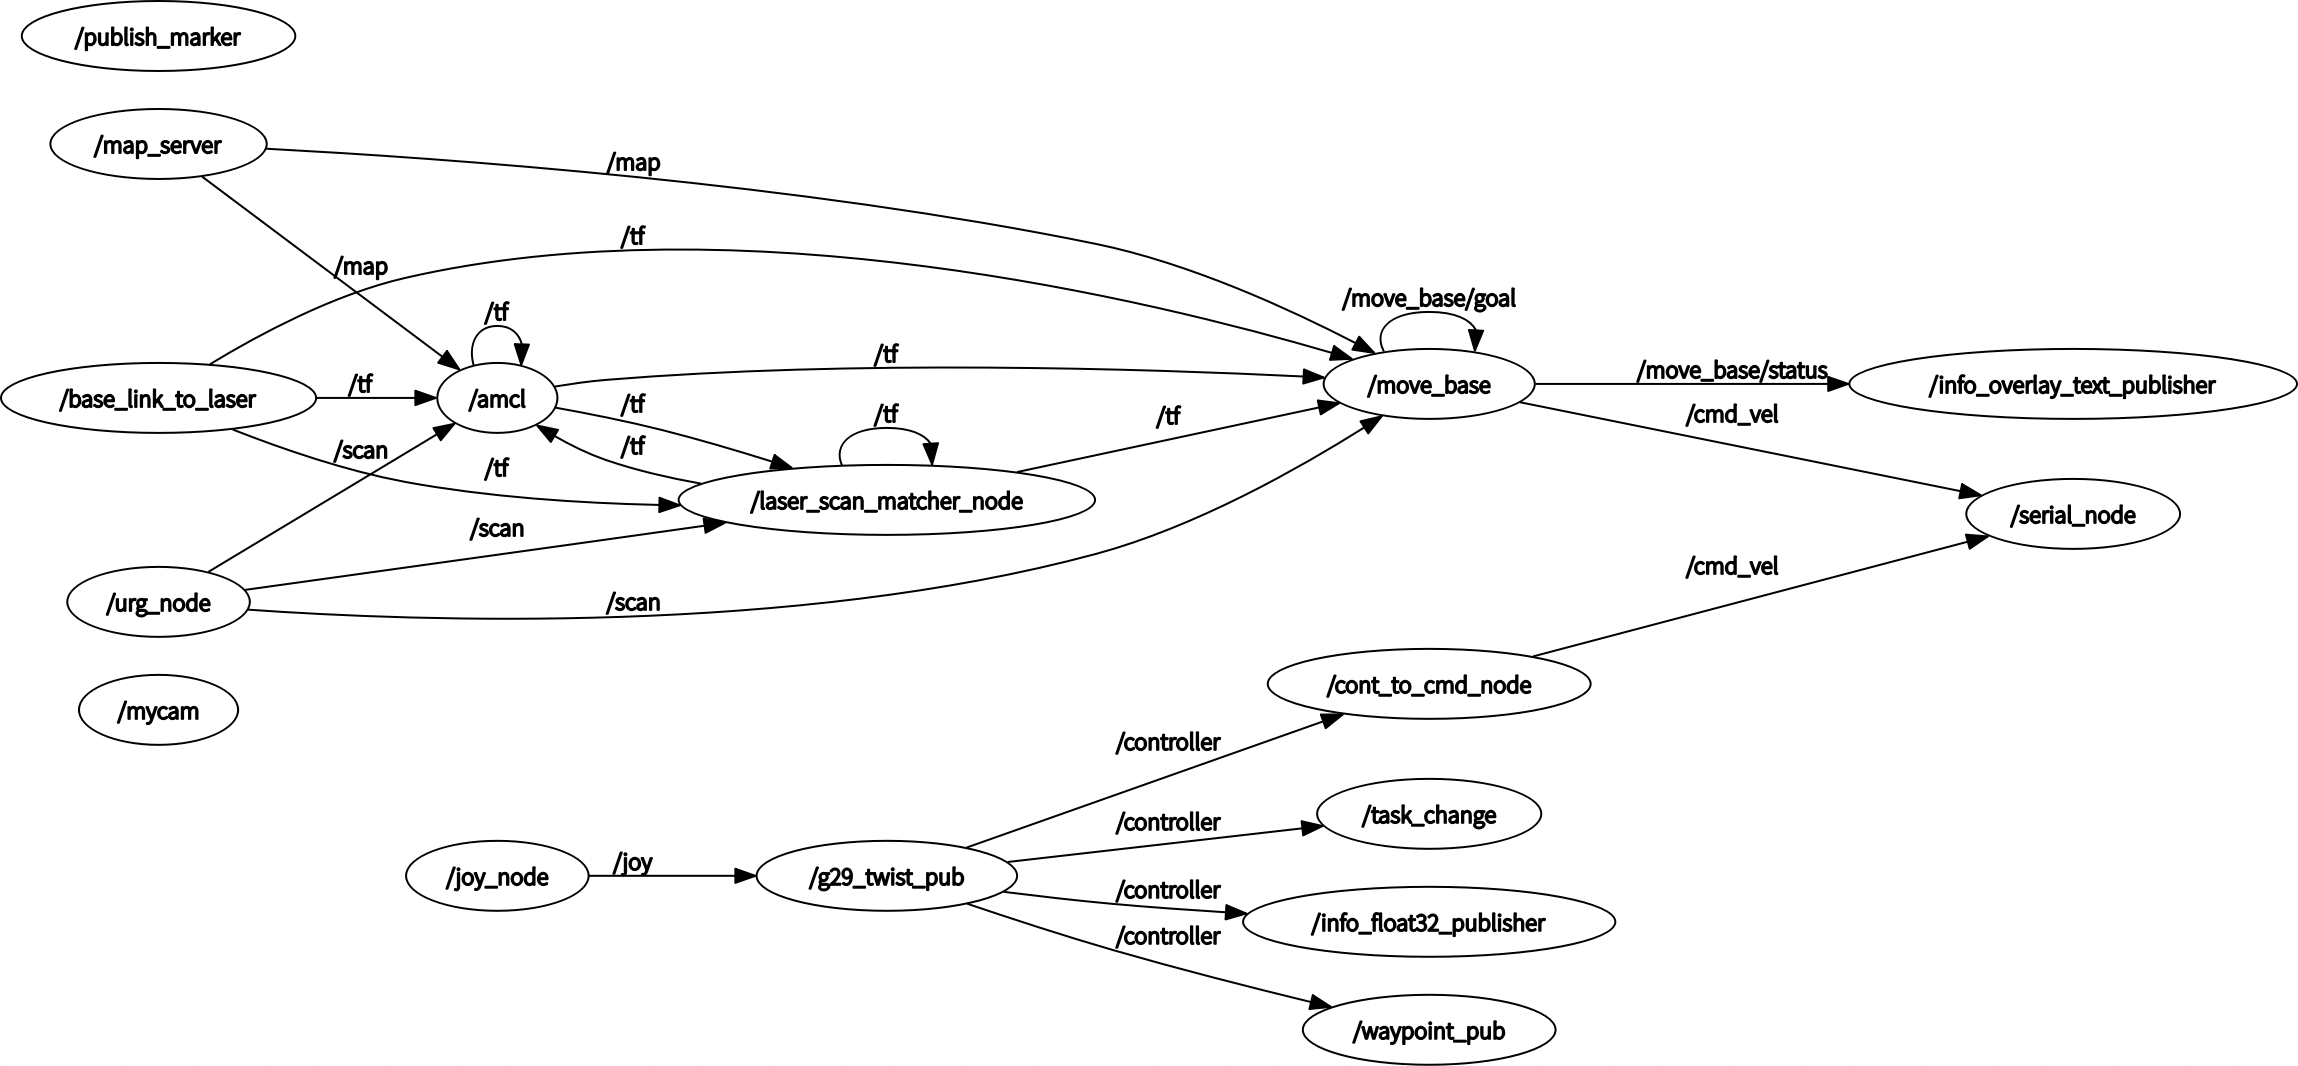
\includegraphics[width=\linewidth]{img/auto_45.png}
    \caption{手動操作時のノード(トピック)}
    \label{auto:change_node}
  \end{center}
\end{figure}

\begin{figure}[h]
  \begin{center}
    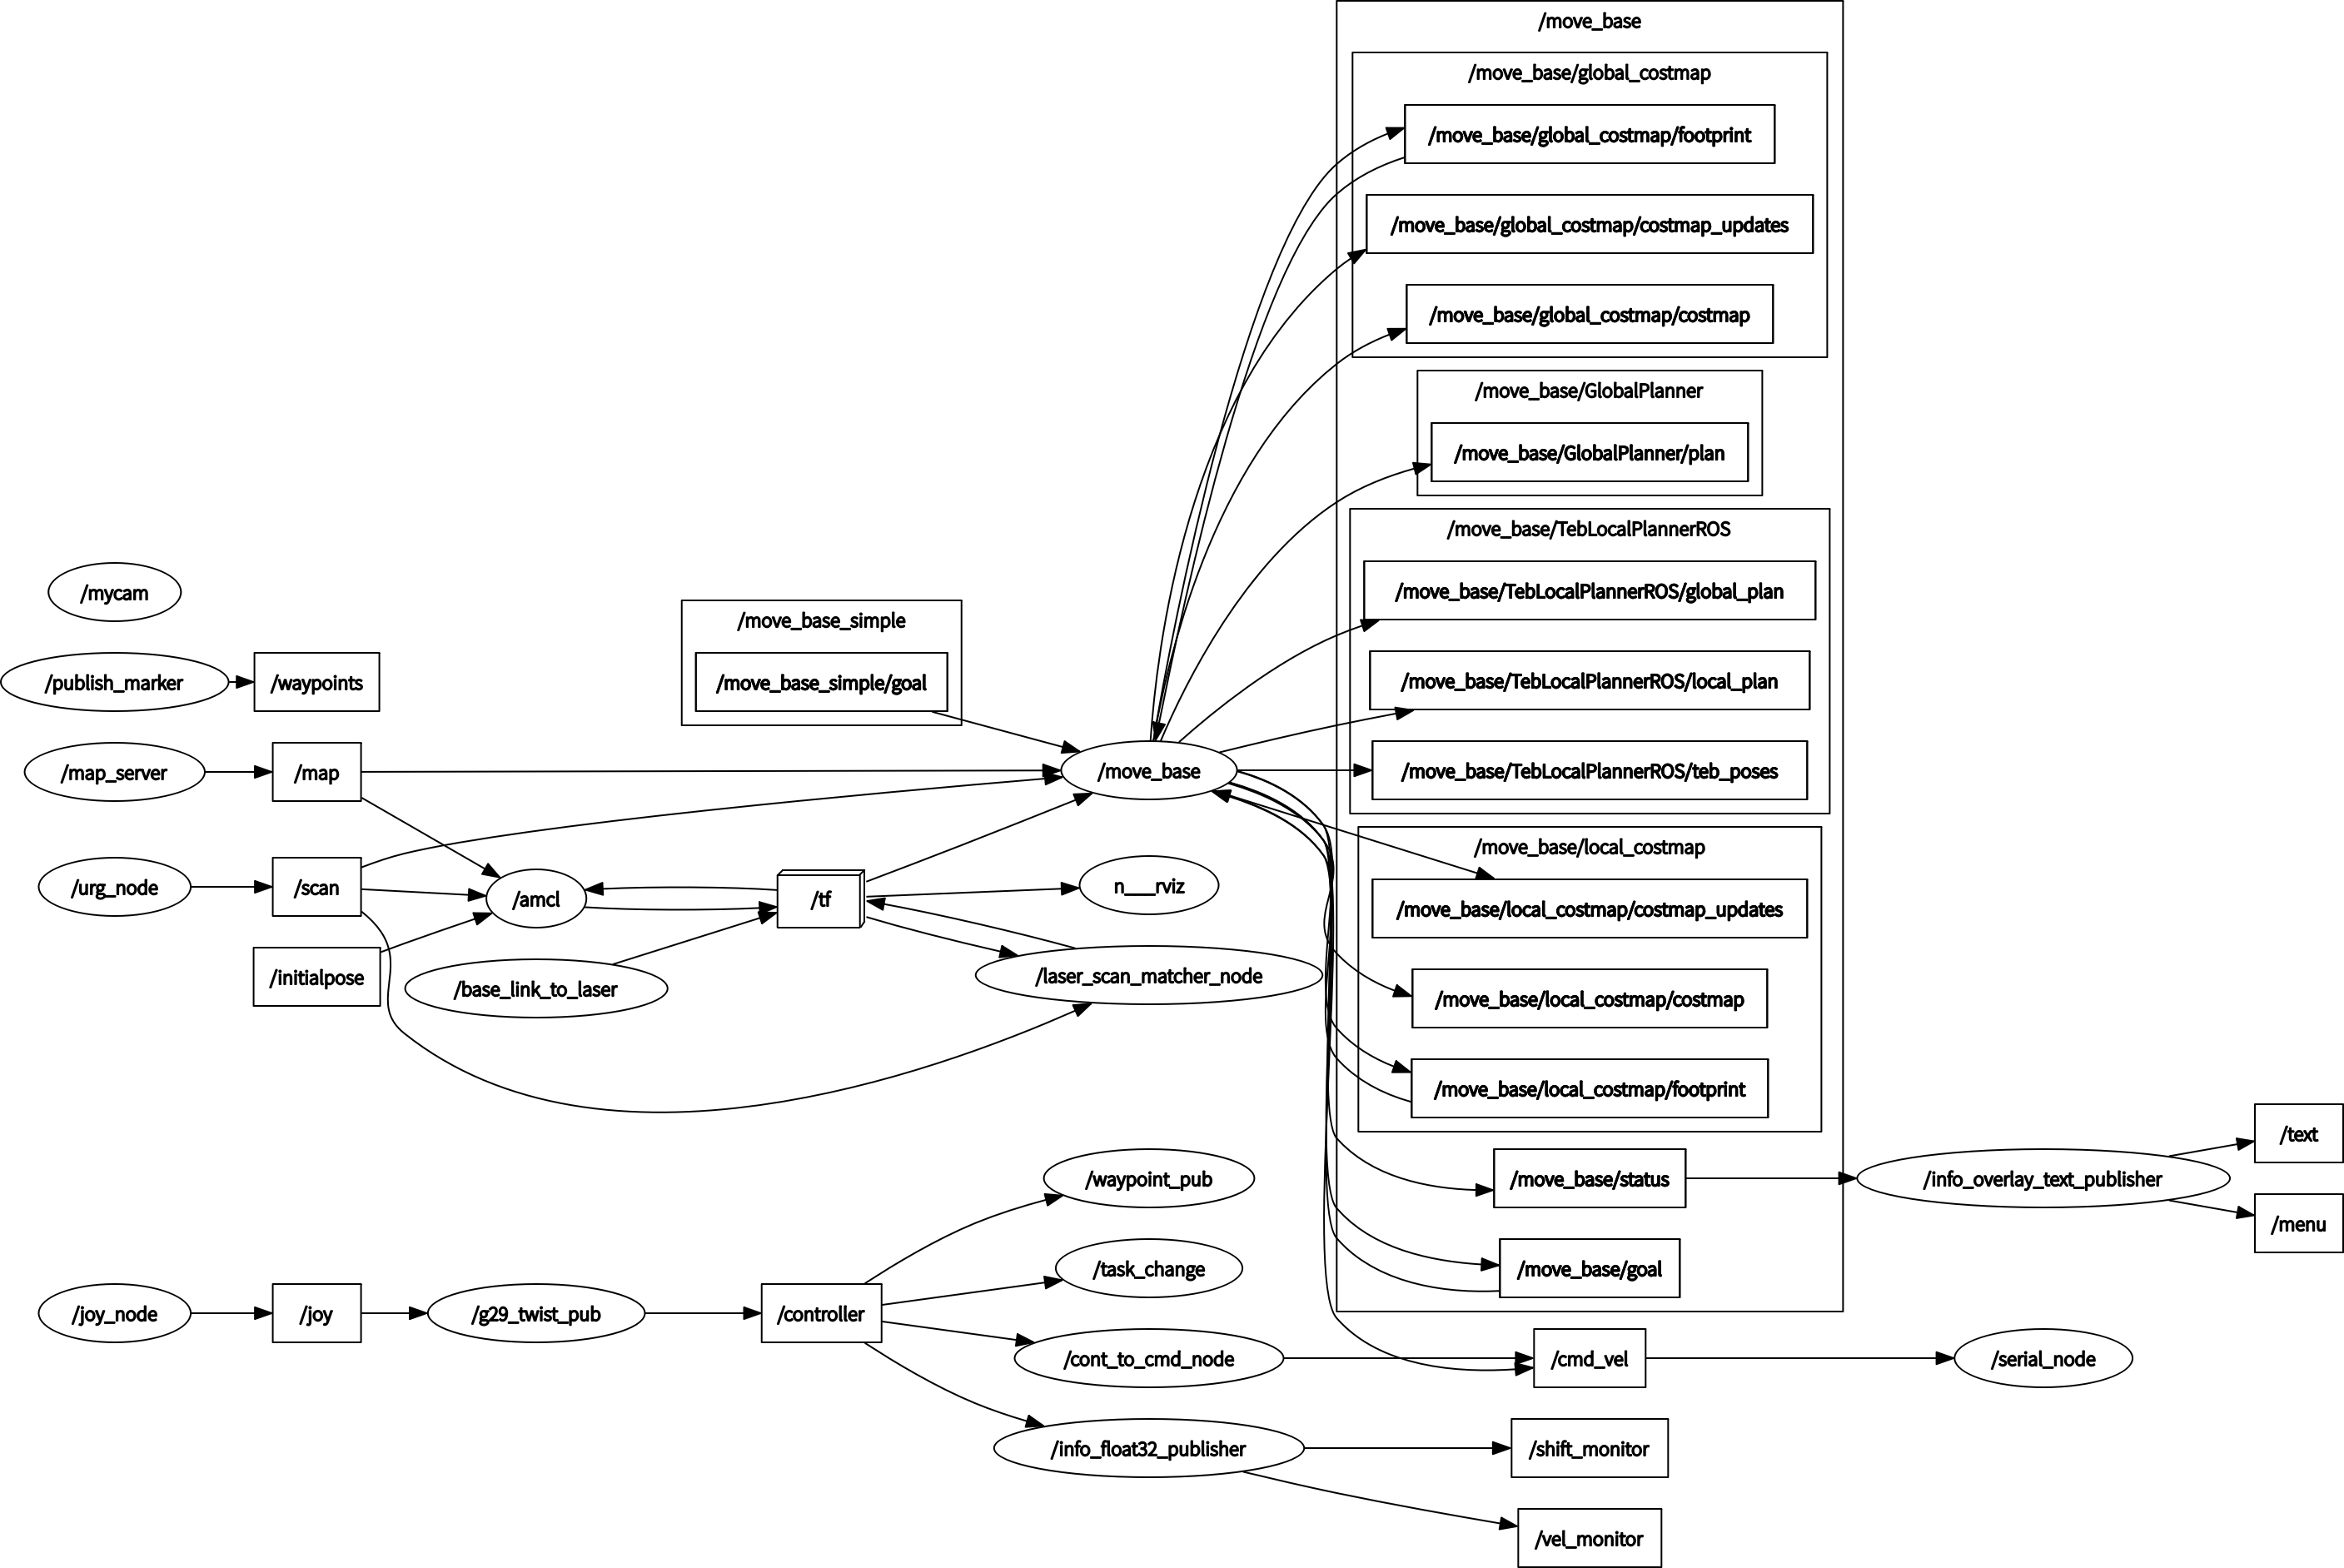
\includegraphics[width=\linewidth]{img/auto_46.png}
    \caption{手動操作時の全体ノード}
    \label{auto:change_node2}
  \end{center}
\end{figure}

\clearpage
\section{検証}
本研究では、以下に示す3つの実験を行った。
\subsection{遠隔操作の操作性の評価}
運転免許不所持者も含めた、運転操作のインタラクションの分析を目的とした遠隔運転の実験を行った。
図\ref{auto:course}にしめす、仕切りの無い走行コースの遠隔操作の体感情報の記録に加えて、ブレーキ操作の記録を行った。
実験の方法として、操作インターフェース(AT/MT/セミAT)を自由に一つ選択し、コースを走行する。その後、図\ref{auto:break}ブレーキテスト
用コースにて、ブレーキテストを実施した。

\begin{figure}[h]
  \begin{center}
    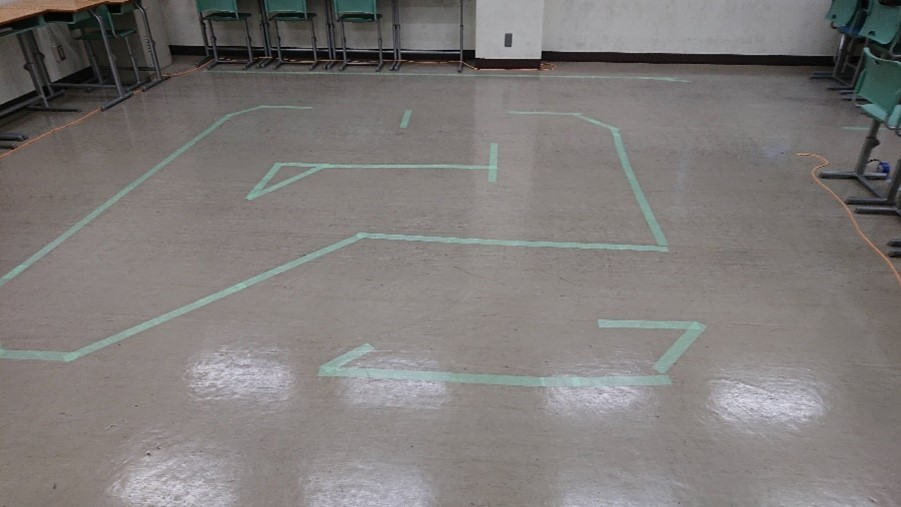
\includegraphics[width=.6\linewidth]{img/auto_47.jpg}
    \caption{仕切りの無い走行コース}
    \label{auto:course}
  \end{center}
\end{figure}

\begin{figure}[h]
  \begin{center}
    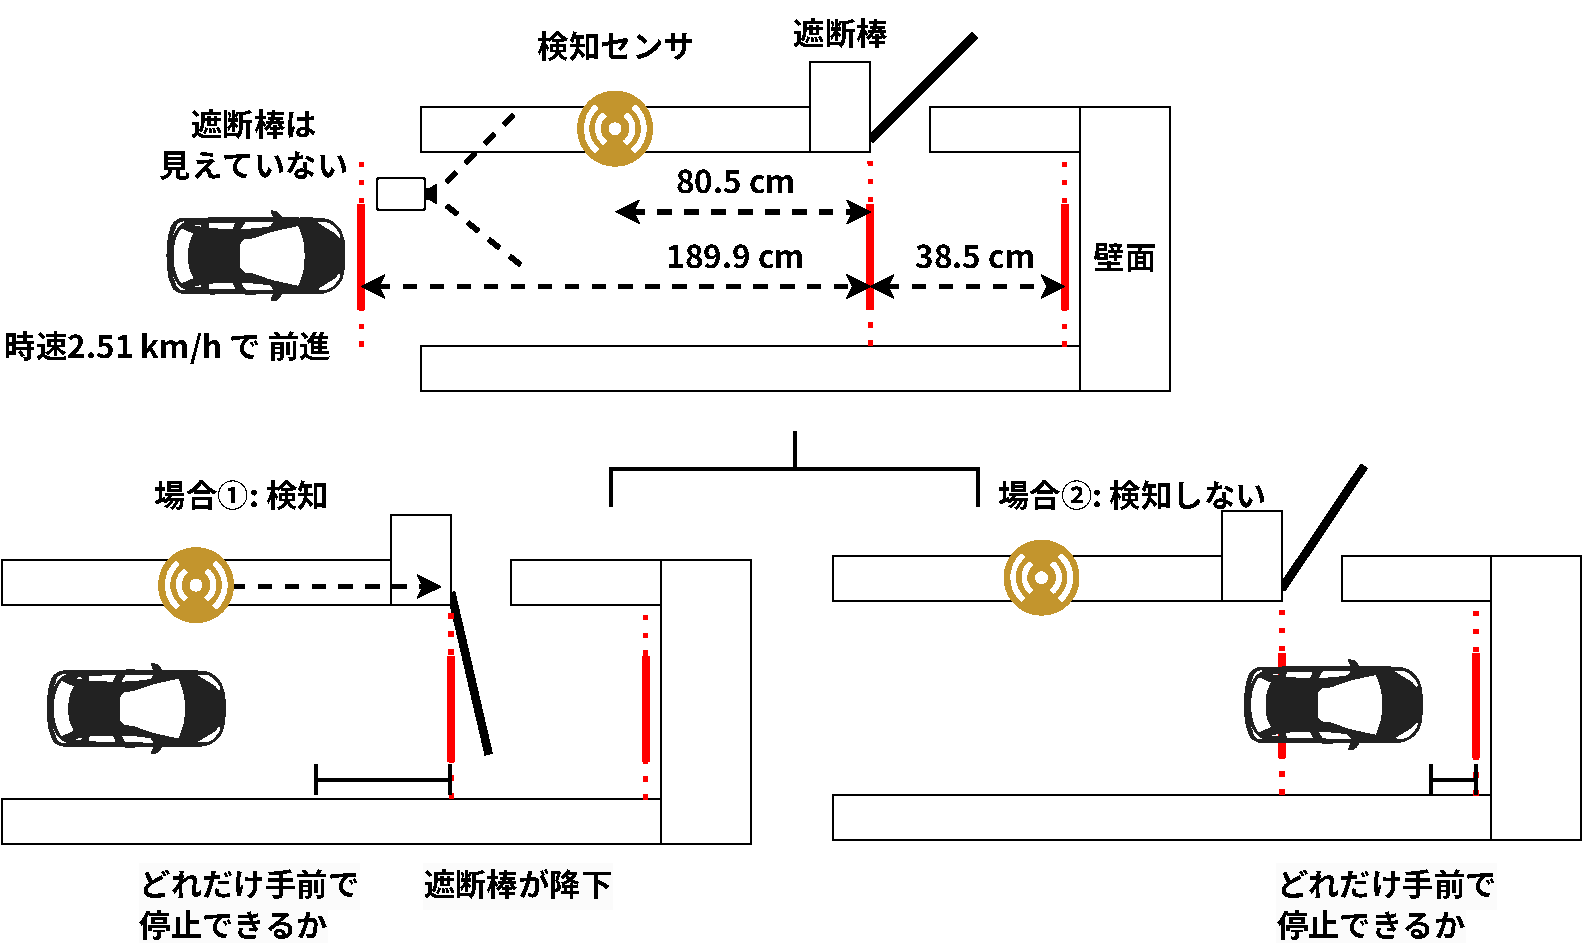
\includegraphics[width=.6\linewidth]{img/auto_48.pdf}
    \caption{ブレーキテストコース}
    \label{auto:break}
  \end{center}
\end{figure}

\subsection{手動運転から自動運転への切り替え}
以下の図\ref{auto:jikken:waypoint}に取得したコースの占有格子地図とwaypointの情報を基に、
手動運転から自動運転への切り替えを行う。具体的には、手動運転から自動運転、それから最後に手動運転に切り替える走行実験を行った。
あらかじめSLAMにより地図を取得して、waypointが設定されている地図上をAMCLによる自己位置推定を行いながら、
手動操作を行う。地図上では、あらかじめ手動から自動に切り替える地点(マップ中の番号0)と、自動から手動に切り替える地点(マップ中の番号3)が明示され、
所定の位置に移動した際に、ステアリングコントローラのモード切り替えスイッチにより、自動運転・手動運転を切り替える操作をして、
コースを周回して、目的値へと操作を行う。

\begin{figure}
  \begin{center}
    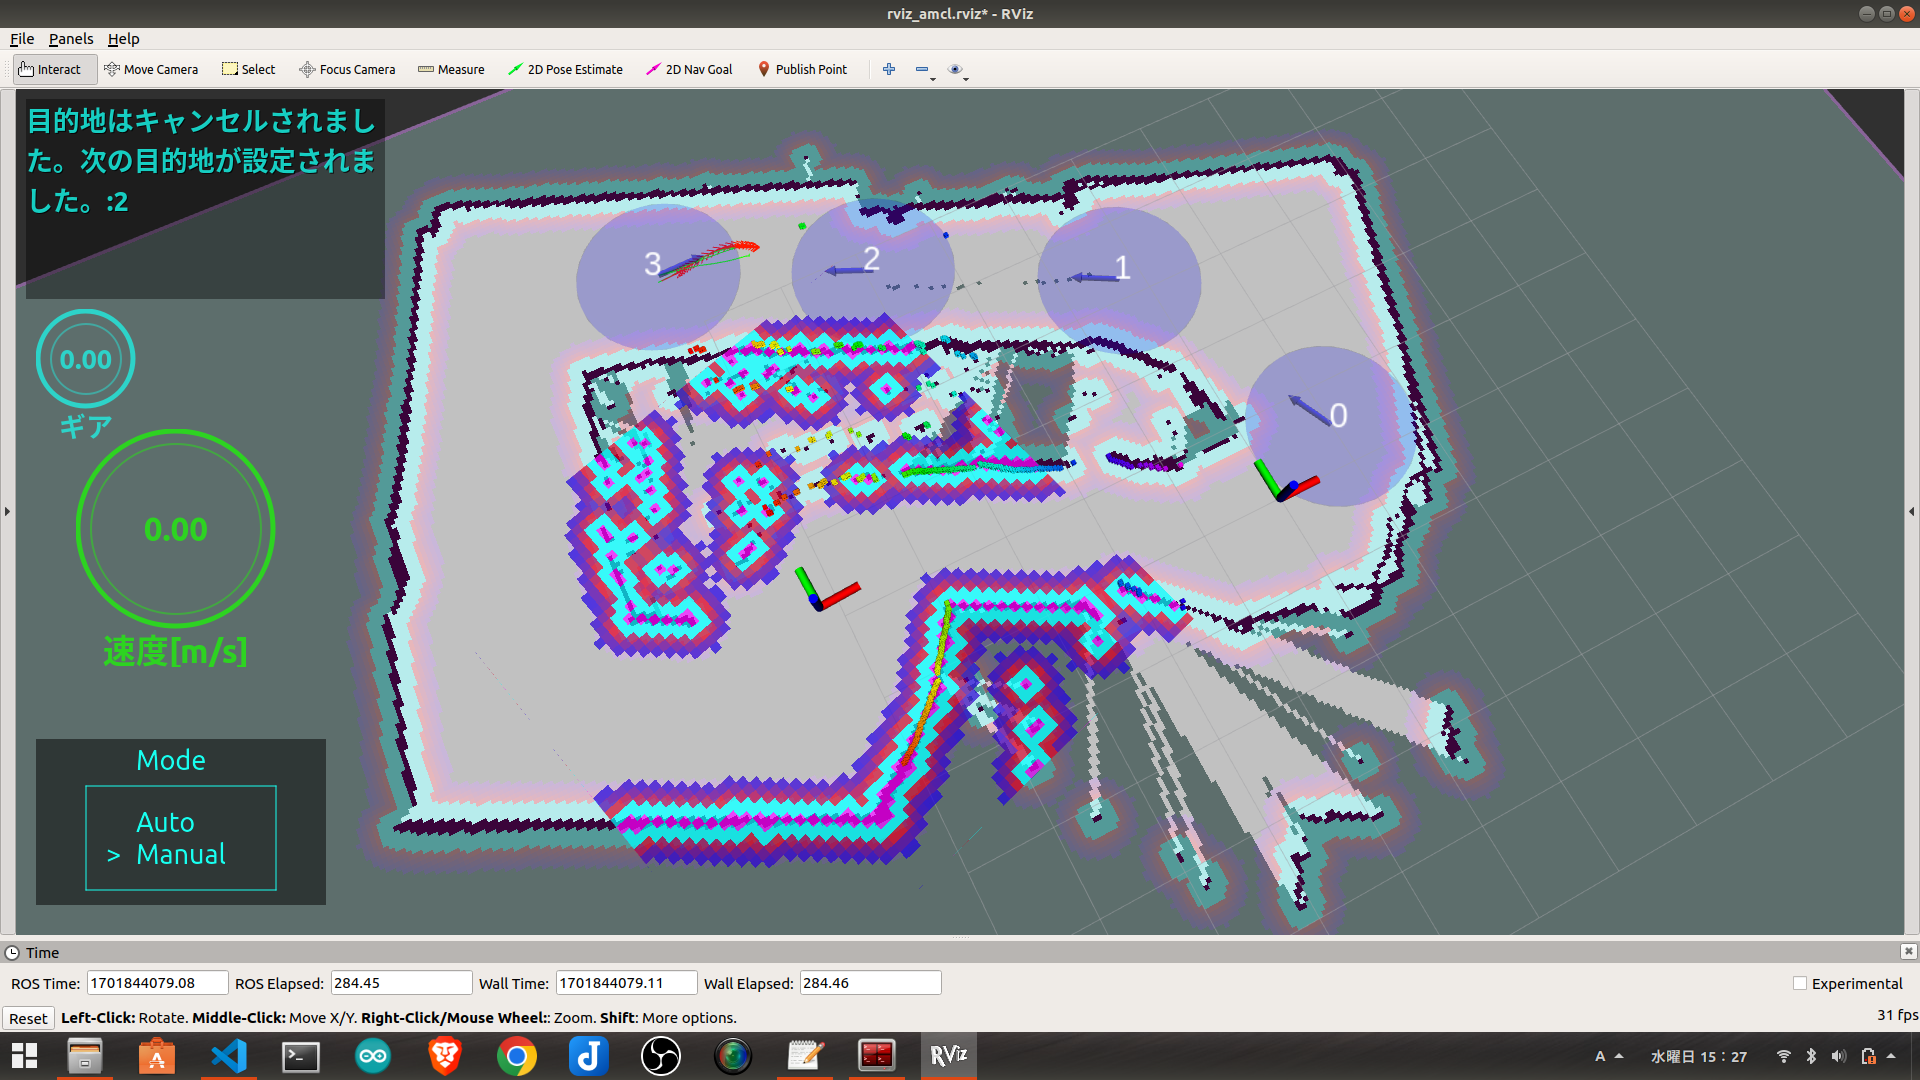
\includegraphics[width=.8\linewidth]{img/auto_49.png}
    \caption{設定したWaypoint}
    \label{auto:jikken:waypoint}
  \end{center}
\end{figure}

\subsection{方向転換機能の評価}
以下の図\ref{auto:tenkan:keiro}に示すコースにおいて、手動操作によって、初期位置から目的値に向けて手動操作を行う。
次に図\ref{auto:tenkan:jikken}のように、自動運転モードで初期位置から目的地に向けて自律移動を行う。走行のパターンは、図\ref{auto:tenkan1}、\ref{auto:tenkan2}に示す2種類
で行う。

\begin{figure}[h]
  \begin{center}
    \subfigure[方向転換のテストコース]{
      \includegraphics[width=.33\linewidth]{img/auto_50.pdf}
      \label{auto:tenkan:keiro}
      }
    \subfigure[方向転換のパターン1]{
      \includegraphics[width=.33\linewidth]{img/auto_51.pdf}
      \label{auto:tenkan1}
    }
    \subfigure[方向転換のパターン2]{
      \includegraphics[width=.33\linewidth]{img/auto_52.pdf}
      \label{auto:tenkan2}
    }
  \caption{方向転換のテストコース}
  \label{auto:tenkan}
  \end{center}
\end{figure}

\begin{figure}
  \begin{center}
    \includegraphics[width=.8\linewidth]{img/auto_53.png}
    \caption{方向転換の自律移動画面}
    \label{auto:tenkan:jikken}
  \end{center}
\end{figure}

\clearpage
\subsection{結果}
\subsubsection{遠隔操作の操作性の評価}
図\ref{auto:result1}\verb|~|\ref{auto:result8}に操作性評価に関する実験結果を示す。
図\ref{auto:result1}の項目に注目すると、被験者が体感した操作がAT、MT、セミATの内いずれが多いかを示す。
アンケートの回答者は46人で、高専祭での一般の来場者に向けたものである。ブレーキテストは、被験者の内33人
がアンケートに回答した。比較的簡単なAT操作を選択した被験者が67\%を占め、その内79\%が操作を難しいと回答した。
また、回答者のうち、若年層(未就学児・小中学生)の被験者が多い。(全体の6 ~ 7割)

\begin{figure}[h]
  \begin{center}
    \subfigure[アンケート1]{
      \includegraphics[width=.45\linewidth]{img/auto_54.pdf}
      \label{auto:result1}
      }
    \subfigure[アンケート2]{
      \includegraphics[width=.45\linewidth]{img/auto_55.pdf}
      \label{auto:result2}
    }
    \subfigure[アンケート3]{
      \includegraphics[width=.45\linewidth]{img/auto_56.pdf}
      \label{auto:result3}
    }
    \subfigure[アンケート4]{
      \includegraphics[width=.45\linewidth]{img/auto_57.pdf}
      \label{auto:result4}
    }
  \caption{アンケート}
  \label{auto:result1_1}
  \end{center}
\end{figure}

\begin{figure}[h]
  \begin{center}
    \subfigure[アンケート1]{
      \includegraphics[width=.45\linewidth]{img/auto_58.pdf}
      \label{auto:result5}
      }
    \subfigure[アンケート2]{
      \includegraphics[width=.45\linewidth]{img/auto_59.pdf}
      \label{auto:result6}
    }
    \subfigure[アンケート3]{
      \includegraphics[width=.45\linewidth]{img/auto_60.pdf}
      \label{auto:result7}
    }
    \subfigure[アンケート4]{
      \includegraphics[width=.45\linewidth]{img/auto_61.pdf}
      \label{auto:result8}
    }
  \caption{アンケート}
  \label{auto:result1_2}
  \end{center}
\end{figure}

\begin{figure}
  \begin{center}
    \includegraphics[width=.8\linewidth]{img/auto_62.pdf}
    \caption{ブレーキテストの結果}
    \label{auto:result1_3}
  \end{center}
\end{figure}

\subsubsection{手動運転から自動運転への切り替え}
手動運転から自動運転への切り替えの実験結果について述べる。手動運転と自動運転の双方への切り替えは
問題なく実施できた。しかし、自律移動の際に、後退状態になると、平坦な直線の後、自己位置が並進方向にずれて見失う
現象であるセンサ退化が起こった。これは、直線が平坦であるため、LiDARのスキャンデータが、地図のどの位置にでもマッチングするためである。
前進状態の場合にも起こるが、自動で補正される場合もあった。しかし、後退時には必ず生じた。

\subsubsection{方向転換機能}
図\ref{auto:result2_2}に方向転換機能の評価の結果を示す。図\ref{auto:tenkan1}、\ref{auto:tenkan2}に示す通りに移動を行うと自己位置が破綻し、
目的地まで到達できない結果であった。具体的には、後退のまま一度に目的地への移動を試みると、最適な経路が得られない。
または、経路の移動中に障害物付近に到達することで停止する。そこで、以下の図\ref{auto:tenkankai1}、\ref{auto:tenkankai2}
のように、自律移動のための経路の分割数を増やし、経路を直線的にすること、さらに、切り返しの分割の際に、転換の方向からやや斜めの姿勢として、
一度に切り返す量を少なくすることで、最終目的値への移動を可能とした。
自律移動シミュレーションでは、切り返しの量を減らす必要がなく、一度で切り返しを行うことができるが、
実機では、異なる結果が得られている。

\begin{figure}[h]
  \begin{center}
    \subfigure[方向転換の改良1]{
      \includegraphics[width=.45\linewidth]{img/auto_63.pdf}
      \label{auto:tenkankai1}
      }
    \subfigure[方向転換の改良2]{
      \includegraphics[width=.45\linewidth]{img/auto_64.pdf}
      \label{auto:tenkankai2}
    }
  \caption{方向転換のパターン改良}
  \label{auto:result2_2}
  \end{center}
\end{figure}

\section{考察}
\subsection{遠隔操作の操作性の評価}
若年層の6\verb|~|7割を占め、AT操作を選択し、同時にハンドル操作に注力したことから、ハンドル操作に慣れていないことが分かる。
特に、若年層の操作を観察すると、カウンター操作(曲がる方向にハンドルを切った後に元に戻す操作)ができないことが明らかになった。一方、大人や、
AT操作と比べて比較的操作の難易度が高い、MT/セミAT操作の選択者は、難なくハンドルを操作した。このことから、操作経験者や熟練者にとっては、
実車よりも操作が簡単であることが推測される。

\subsection{手動運転から自動運転への切り替え}
手動運転から自動運転に切り替える際の待ち時間が1秒程度であり、その間停止する。手動から自動への切り替えは機能した。
今回は問題なく機能したが、手動操作の間隔には遅延が生じたため、応答速度が速い場合に影響が生じる可能性があると考えられる。

\subsection{方向転換機能の評価}
LiDARのみのSLAMで作成した地図は、歪んでいたが、特徴量に矛盾が無かったため、LiDARのレーザオドメトリとのスキャンマッチングが上手く機能することで、
自己位置を見失いにくく、自律移動が実施できたと考えられる。切り返しの分割の際に、転換の方向からやや斜めの姿勢として、一度に切り返す量を少なくすることで、
最終目的地への移動を可能とした。これは、実際の人による車両操作に近く、最も衝突のリスクが少ない方法と考えられる。
このことから、LiDARのみのSLAMで作成した環境地図は、精度が低くても、特徴量に矛盾が無ければ、目的地への自律移動は、中継地点を複数設定することで実現されることが明らかになった。
また、自律移動シミュレーションでは、切り返しの量を減らす必要がなく、一度の目的地設定により、最適な切り返しを行うことができるが、
実機では、目的地を複数設定し、切り返しの頻度を増やす必要がある点については、地図に含まれる測定誤差や、LiDARの測定誤差等による影響で、
自己位置推定に影響を受けているためだと考えられる。

\section{おわりに}
本研究では、RCカーの遠隔操作と自律移動を切り替える機能を有する、自動運転システムを開発し、その使用性を評価した。遠隔操作は、ステアリングコントローラのハンドルの左右の入力による、旋回機能、アクセルペダルの押下による前進機能、シフトレバーによるトランスミッションのモード切り替えによる後退機能と、ブレーキペダルの押下による減速機能を実現した。また、AT操作のみではなく、MT操作やセミオートマ機能を搭載し、実車と同等の操作感覚で操作を行うことができるシステムを実現した。自動運転システムは、LiDARのみによるSLAMと、Navigation Stackを用いたWaypoint Navigationを実現した。手動運転・自動運転の切り替え機能は、遠隔操作と、自律移動のタスクの切り替えをステアリングコントローラから行うことで実現した。使用性の評価において、遠隔操作においては、個々の運転技能に応じたインターフェースによって、実機でのインタラクションを実現し、若年層に向けたステアリング操作の補正が必要であることが明らかになった。また、自動運転機能を用いた手動・運転引継ぎの実験では、問題なく引継ぎが行えることが明らかになった。また、従来の車型自律移動システムでは、検証されなかった、後退機能に関する切り返し動作の評価を行った。その結果、一度に目的地に到達するために、切り返す回数を少なくするのではなく、切り返す回数を増やすことで、LiDARのみでのナビゲーションが可能であることが明らかになった。自律移動の際に、特徴量の少ない経路を通る際に、LiDARのみによるオドメトリではセンサの退化により、自己位置を見失う現象が生じたが、特徴量が多い点であれば、スキャンマッチングが機能したことから、特徴量の多い地図ならば、LiDARのみによるSLAMはある程度可能であることが明らかになった。

本研究では、屋内環境での実験であり、屋外での利用を想定していない。具体的には、屋外では、地図が膨大になるため、複数の地図を用意する必要があり、自律移動の度に、切り替える機能が必要となる。今後は、屋外自律移動を目的として、地図の切り替え機能の実装を検討する。